%%%%%%%%%%%%%%%%%%%%%%%%%%%%%%%%%%%%%%%%%%%%%%%%%%%%%%%%%%%
%\section{Example cases}
%%%%%%%%%%%%%%%%%%%%%%%%%%%%%%%%%%%%%%%%%%%%%%%%%%%%%%%%%%%
%
%
%%%%%%%%%%%%%%%%%%%%%%%%%%%%%%%%%%%%%%%%%%%%%%%%%%%%%%%%%%%
\subsection{Descendant: proxies (a)}
%%%%%%%%%%%%%%%%%%%%%%%%%%%%%%%%%%%%%%%%%%%%%%%%%%%%%%%%%%%
%
%
\begin{frame}[t, negative]
	\subsectionpage
\end{frame}
%
%
\begin{frame}
	{Proxies (a)\footnote{\citet{McElreath_2020}, chapter 11 (p. 340); \citet{McElreath_2022}, lecture 10}}
	%
	\begin{columns}
		%
		\begin{column}{0.5\textwidth}
			%
			research question, 
			%
			\begin{itemize}
				%
				\item \textcolor{blue}{Does $X$ has a (direct) effect on $M$?}
				%
			\end{itemize}
			
			variables,
			%
			\begin{itemize}
				%
				\item X, teacher experience
				\item E, instruction quality (old, new) \\
				{\small (unobserved)}
				\item A, proxy variable (e.g. age)
				\item M, teachers' score in mathematics \\
				{\small (from a standardized evaluation)}
				%
			\end{itemize}
			%
		\end{column}
		%
		\begin{column}{0.5\textwidth}  
			%
			\begin{equ}
				%
				M = \left\{ \begin{aligned} 
					A \leftarrow & \; f_{A}(E,U_{A}) \\
					X \leftarrow & \; f_{X}(E,U_{X}) \\
					M \leftarrow & \; f_{M}(E, X, U_{M})\\
					U \sim & \; P(\pmb{U})
				\end{aligned} \right
				%
				\caption*{(a) structural model}
				%
			\end{equ}
			%
			\begin{figure}
				%
				\begin{tikzpicture}
					% nodes
					\node[formula] at (-2,0) {$U_{X}$};
					\node[formula] at (-1,-0.3) {$X$};
					\node[formula] at (0,1) {$E$};
					\node[formula] at (1,1) {$A$};
					\node[formula] at (2,0.75) {$U_{A}$};
					\node[formula] at (1,-0.3) {$M$};
					\node[formula] at (2,0) {$U_{M}$};
					
					% paths
					\draw [{Circle [open]}-{latex}](-1.7,0)--(-1,0); % Ux->X
					\draw [{Circle}-{latex}](-1.03,0)--(0.9,0); % X->L
					\draw [{Circle [open]}-{latex}{Circle}](1.7,0)--(0.9,0); % Um->M
					\draw [-{latex}](0,0.75)--(-0.95,0.05); % E->X
					\draw [{Circle [open]}-{latex}](0,0.8)--(0.9,0.05); % E->M
					\draw [-{latex}](0.1,0.75)--(0.90,0.75); % E->A
					\draw [{Circle [open]}-{latex}{Circle}](1.7,0.75)--(0.9,0.75); % Ul->U2
					
					% extra
					\node at (0,-0.25) {$(?)$}; % symbol
				\end{tikzpicture}
				%
				\caption*{(b) causal diagram}
				%
			\end{figure}
			%
		\end{column}
		%
	\end{columns}
	%
\end{frame}
%
%
\begin{frame}
	{Simulation setting}
	%
	\begin{columns}
		%
		\begin{column}{0.5\textwidth}
			%
			\begin{figure}
				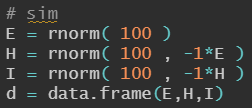
\includegraphics[scale=0.8]{descendant1_code.png}
				\caption*{(c) R code}
			\end{figure}
			%
			\textcolor{blue}{Implications},
			%
			\begin{itemize}
				\item \ndsep{A}{M} \\
				\item \ndsep{A}{X} \\
				\item \dsep{X}{M} \; | E {\small (impossible)}
				\item \dsep{X}{M} \; | A {\small (partially)}
			\end{itemize}
			%
		\end{column}
		%
		\begin{column}{0.5\textwidth}  
			%
			\begin{equ}
				%
				M = \left\{ \begin{aligned} 
					A \leftarrow & \; f_{A}(E,U_{A}) \\
					X \leftarrow & \; f_{X}(E,U_{X}) \\
					M \leftarrow & \; f_{M}(E, X, U_{M})\\
					U \sim & \; P(\pmb{U})
				\end{aligned} \right
				%
				\caption*{(a) structural model}
				%
			\end{equ}
			%
			\begin{figure}
				%
				\begin{tikzpicture}
					% nodes
					\node[formula] at (-2,0) {$U_{X}$};
					\node[formula] at (-1,-0.3) {$X$};
					\node[formula] at (0,1) {$E$};
					\node[formula] at (1,1) {$A$};
					\node[formula] at (2,0.75) {$U_{A}$};
					\node[formula] at (1,-0.3) {$M$};
					\node[formula] at (2,0) {$U_{M}$};
					
					% paths
					\draw [{Circle [open]}-{latex}{Circle}](-1.7,0)--(-0.9,0); % Ux->X
					%\draw [{Circle}-{latex}](-1.03,0)--(0.9,0); % X->M
					\draw [{Circle [open]}-{latex}{Circle}](1.7,0)--(0.9,0); % Um->M
					\draw [-{latex}](0,0.75)--(-0.95,0.05); % E->X
					\draw [{Circle [open]}-{latex}](0,0.8)--(0.9,0.05); % E->M
					\draw [-{latex}](0.1,0.75)--(0.90,0.75); % E->A
					\draw [{Circle [open]}-{latex}{Circle}](1.7,0.75)--(0.9,0.75); % UA->A
				\end{tikzpicture}
				%
				\caption*{(b) causal diagram}
				%
			\end{figure}
			%
		\end{column}
		%
	\end{columns}
	%
\end{frame}
%
%
\begin{lhframe}[rhgraphic={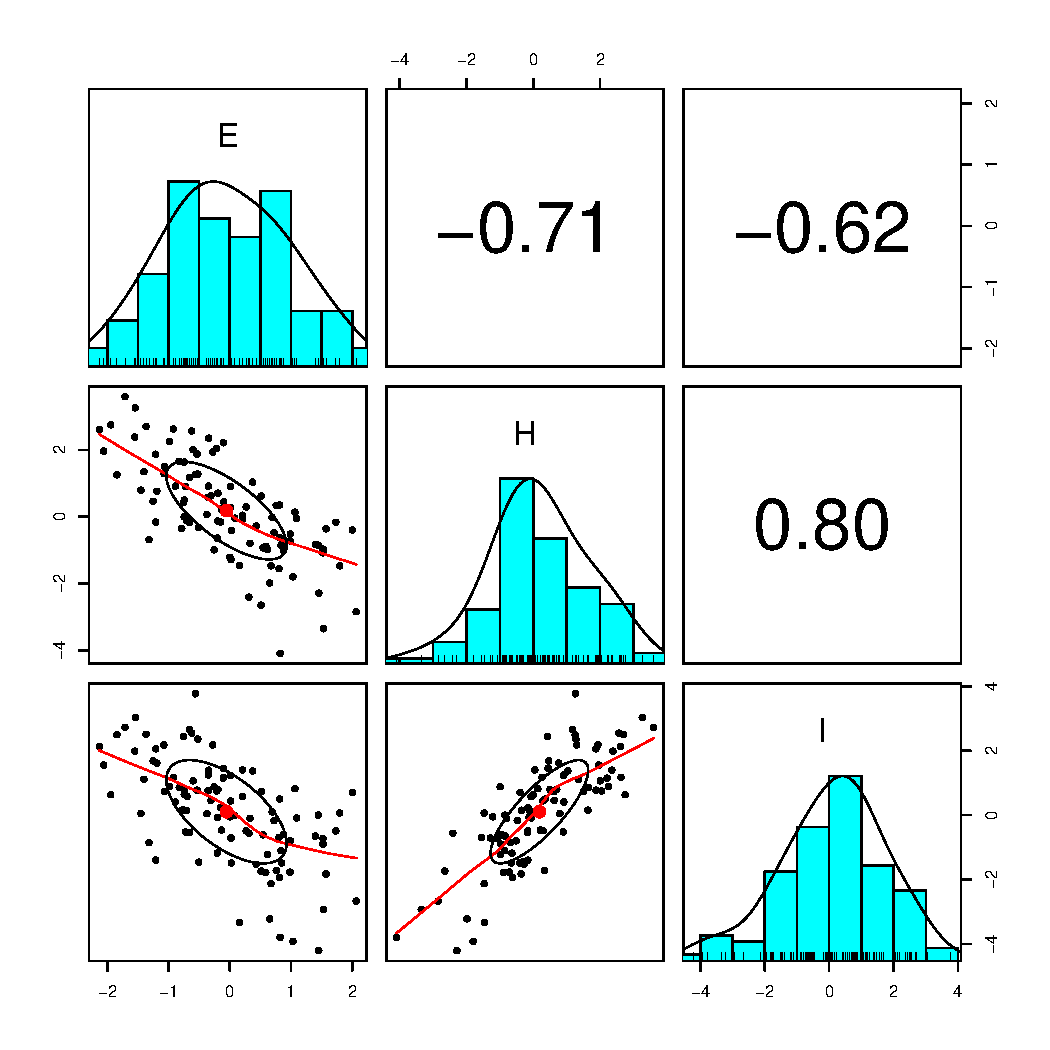
\includegraphics[scale=0.4]{descendant1_panel.pdf}}]
	{``Eyeballing" analysis}
	
	based on \textcolor{blue}{correlation analysis},
	%
	\begin{itemize}
		%
		\item $Cor(A,M)<0$ goes in line with our ``rudimentary" understanding of the data, \\
		{\small (old teachers has old type of instruction, and lower score)}
		%
		\item but $cor(X, M)<0$ does not go in line with our ``understanding"\\
		{\small (the more experienced, the less the score?)}
		%
		\item but we \textcolor{blue}{might include} $Z$ in our statistical model \\
		{\small (based on univariate (linear) correlation)}
		%
	\end{itemize}
	%
\end{lhframe}
%
%
\begin{lhframe}[rhgraphic={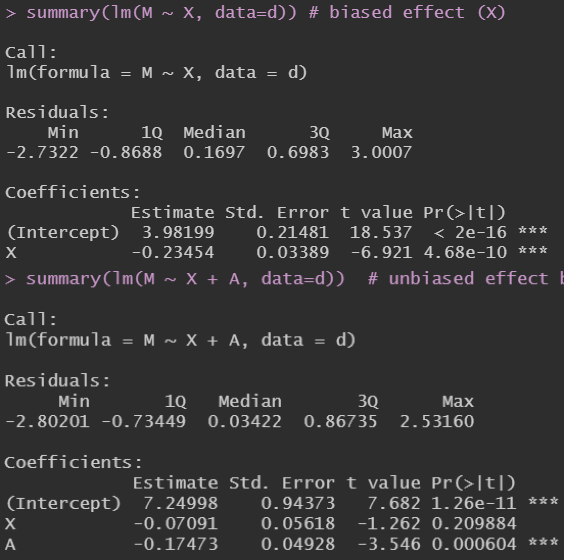
\includegraphics[scale=0.3]{descendant1_reg.png}}]
	{Regression, regression!!}
	
	based on \textcolor{blue}{statistical analysis},
	%
	\begin{itemize}
		%
		\item we now have two models with two different effects
		\item which one is the ``truth"?
		%
	\end{itemize}
	%
\end{lhframe}
%
%
\begin{lhframe}[rhgraphic={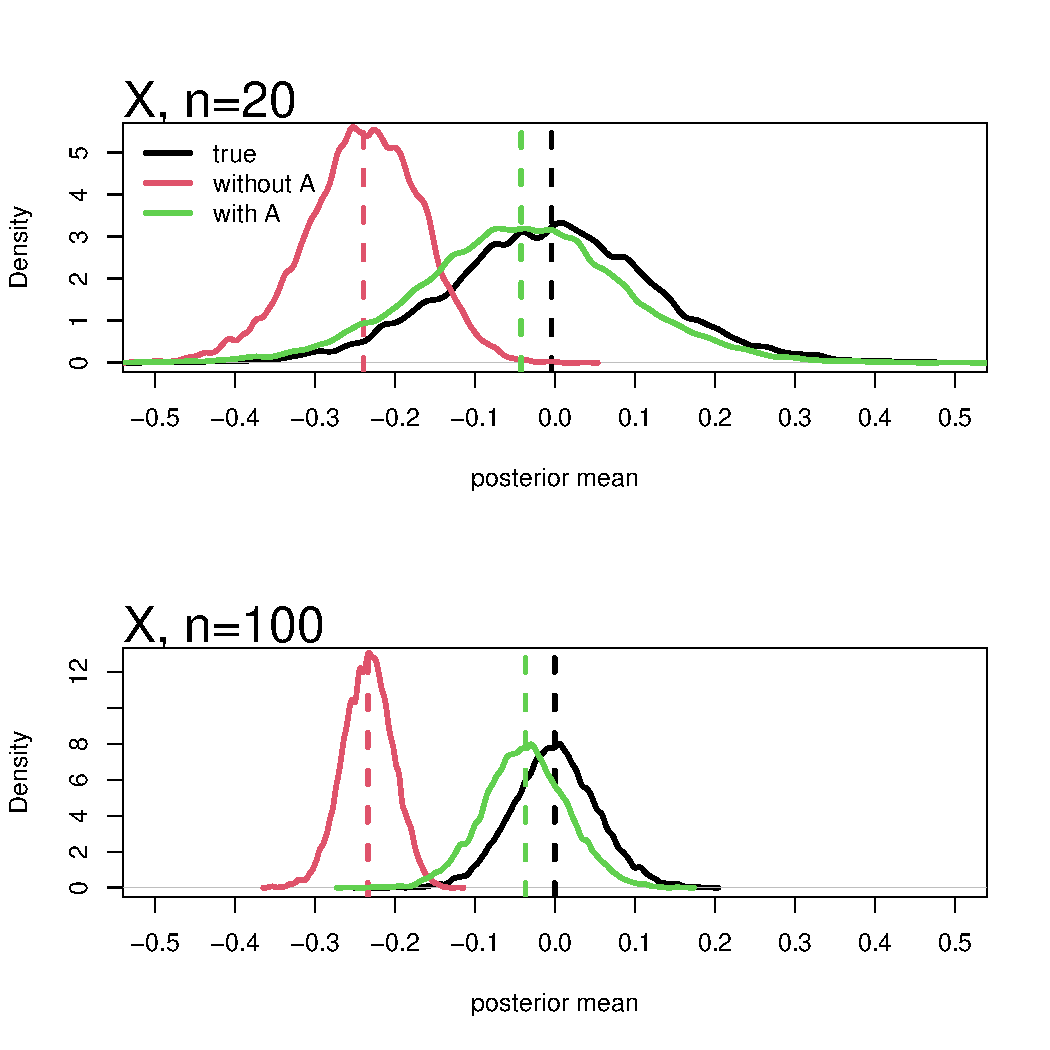
\includegraphics[scale=0.45]{descendant1a_samplesize.pdf}}]
	{The data tell-tell story!!}
	
	imagine we can continue sampling,
	%
	\begin{itemize}
		%
		\item top: $10,000$ samples $n=20$
		\item bottom: $10,000$ samples $n=100$
		%
	\end{itemize}
	
	the larger the sample size,
	%
	\begin{itemize}
		%
		\item under the model \textcolor{blue}{without $A$}, \\
		the more \textcolor{blue}{certain} you are about your \textcolor{blue}{biased} estimates
		%
		\item under the model \textcolor{blue}{with $A$}, \\
		the more \textcolor{blue}{certain} you are about your \textcolor{blue}{less biased} estimates
		%
	\end{itemize}
	%
\end{lhframe}
%
%
\begin{frame}
	{So, what is going on?}
	%
	\begin{columns}
		%
		\begin{column}{0.5\textwidth}
			%
			based on \textcolor{blue}{DAG} and \textcolor{blue}{statistical model},
			%
			\begin{itemize}
				%
				\item stratifying on $A$ \textcolor{blue}{partially blocks} the backdoor path produced by the confounder $E$ \\
				i.e. when stratifying by $A$ you are partially stratifying by $E$
				%
			\end{itemize}
			%
		\end{column}
		%
		\begin{column}{0.5\textwidth}  
			%
			\begin{equ}
				%
				M = \left\{ \begin{aligned} 
					A \leftarrow & \; f_{A}(E,U_{A}) \\
					X \leftarrow & \; f_{X}(E,U_{X}) \\
					M \leftarrow & \; f_{M}(E, X, U_{M})\\
					U \sim & \; P(\pmb{U})
				\end{aligned} \right
				%
				\caption*{(a) structural model}
				%
			\end{equ}
			%
			\begin{figure}
				%
				\begin{tikzpicture}
					% nodes
					\node[formula] at (-2,0) {$U_{X}$};
					\node[formula] at (-1,-0.3) {$X$};
					\node[formula] at (0,1) {$E$};
					\node[formula] at (1,1) {$A$};
					\node[formula] at (2,0.75) {$U_{A}$};
					\node[formula] at (1,-0.3) {$M$};
					\node[formula] at (2,0) {$U_{M}$};
					
					% paths
					\draw [{Circle [open]}-{latex}](-1.7,0)--(-1,0); % Ux->X
					\draw [{Circle}-{latex}](-1.03,0)--(0.9,0); % X->L
					\draw [{Circle [open]}-{latex}{Circle}](1.7,0)--(0.9,0); % Um->M
					\draw [-{latex}](0,0.75)--(-0.95,0.05); % E->X
					\draw [{Circle [open]}-{latex}](0,0.8)--(0.9,0.05); % E->M
					\draw [-{latex}](0.1,0.75)--(0.90,0.75); % E->A
					\draw [{Circle [open]}-{latex}{Circle}](1.7,0.75)--(0.9,0.75); % Ul->U2
					
					% extra
					\node at (0,-0.25) {$(?)$}; % symbol
				\end{tikzpicture}
				%
				\caption*{(b) causal diagram}
				%
			\end{figure}
			%
		\end{column}
		%
	\end{columns}
	%
\end{frame}
%
%
\begin{lhframe}[rhgraphic={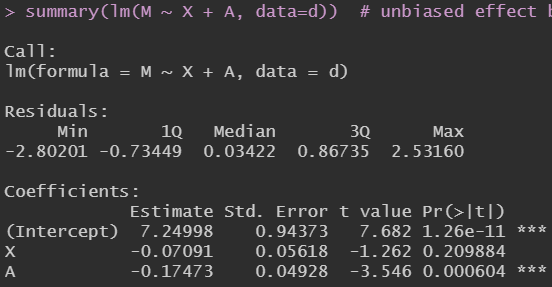
\includegraphics[scale=0.52]{descendant1_reg2.png}}]
	{the dream team!!}
	
	based on \textcolor{blue}{DAG} and \textcolor{blue}{statistical analysis},
	%
	\begin{itemize}
		%
		\item the less biased model is the second, \\
		{\small \textcolor{blue}{(assuming our DAG is true)} }
		%
	\end{itemize}
	%
\end{lhframe}
%
%
\begin{frame}
	{But age cause experience, right?}
	%
	\begin{columns}
		%
		\begin{column}{0.5\textwidth}
			%
			research question, 
			%
			\begin{itemize}
				%
				\item \textcolor{blue}{Does $X$ has a (direct) effect on $M$?}
				%
			\end{itemize}
			
			variables,
			%
			\begin{itemize}
				%
				\item X, teacher experience
				\item E, instruction quality (old, new) \\
				{\small (unobserved)}
				\item A, cause variable (e.g. age)
				\item M, teachers' score in mathematics \\
				{\small (from a standardized evaluation)}
				%
			\end{itemize}
			%
		\end{column}
		%
		\begin{column}{0.5\textwidth}  
			%
			\begin{equ}
				%
				M = \left\{ \begin{aligned} 
					A \leftarrow & \; f_{A}(U_{A}) \\
					X \leftarrow & \; f_{X}(E,U_{X}) \\
					M \leftarrow & \; f_{M}(E, X, U_{M})\\
					U \sim & \; P(\pmb{U})
				\end{aligned} \right
				%
				\caption*{(a) structural model}
				%
			\end{equ}
			%
			\begin{figure}
				%
				\begin{tikzpicture}
					% nodes
					\node[formula] at (-2,0) {$U_{X}$};
					\node[formula] at (-1,-0.3) {$X$};
					\node[formula] at (0,1) {$E$};
					\node[formula] at (1,1) {$A$};
					\node[formula] at (2,0.75) {$U_{A}$};
					\node[formula] at (1,-0.3) {$M$};
					\node[formula] at (2,0) {$U_{M}$};
					
					% paths
					\draw [{Circle [open]}-{latex}](-1.7,0)--(-1,0); % Ux->X
					\draw [{Circle}-{latex}](-1.03,0)--(0.9,0); % X->L
					\draw [{Circle [open]}-{latex}{Circle}](1.7,0)--(0.9,0); % Um->M
					\draw [-{latex}](0,0.75)--(-0.95,0.05); % E->X
					\draw [{Circle [open]}-{latex}](0,0.8)--(0.9,0.05); % E->M
					\draw [-{latex}](0.90,0.75)--(0.1,0.75); % A->E
					\draw [{Circle [open]}-{latex}{Circle}](1.7,0.75)--(0.9,0.75); % Ul->U2
					
					% extra
					\node at (0,-0.25) {$(?)$}; % symbol
				\end{tikzpicture}
				%
				\caption*{(b) causal diagram}
				%
			\end{figure}
			%
		\end{column}
		%
	\end{columns}
	%
\end{frame}
%
%
\begin{lhframe}[rhgraphic={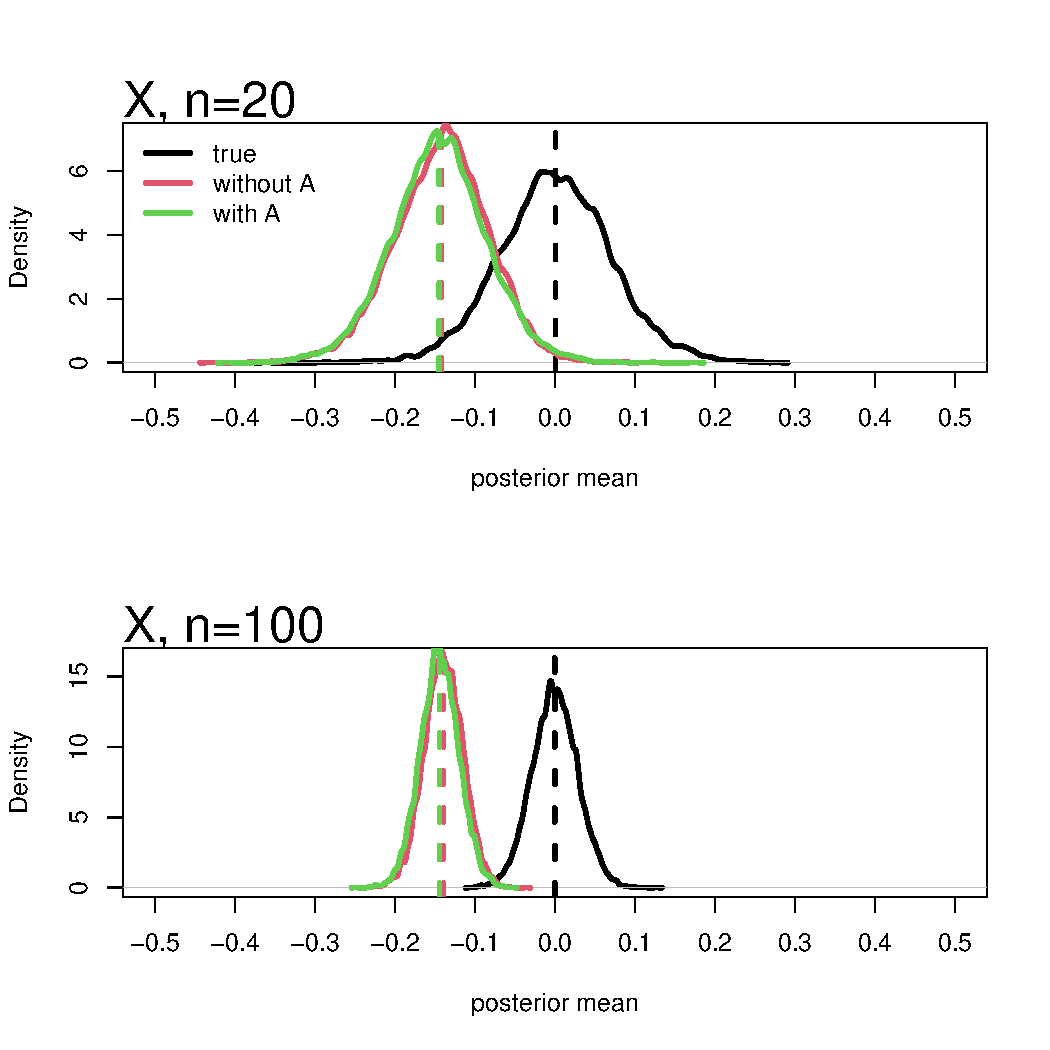
\includegraphics[scale=0.45]{descendant1b_samplesize.pdf}}]
	{But age cause experience, right?}
	
	imagine we can continue sampling,
	%
	\begin{itemize}
		%
		\item top: $10,000$ samples $n=20$
		\item bottom: $10,000$ samples $n=100$
		%
	\end{itemize}
	
	the larger the sample size,
	%
	\begin{itemize}
		%
		\item under any model including $A$, \\
		the more \textcolor{blue}{certain} you are about your \textcolor{blue}{biased} estimates
		%
	\end{itemize}
	%
\end{lhframe}
%
%

\begin{comment}

%%%%%%%%%%%%%%%%%%%%%%%%%%%%%%%%%%%%%%%%%%%%%%%%%%%%%%%%%%%
\subsection{Descendant: proxies (b)}
%%%%%%%%%%%%%%%%%%%%%%%%%%%%%%%%%%%%%%%%%%%%%%%%%%%%%%%%%%%
%
%
\begin{frame}[t, negative]
	\subsectionpage
\end{frame}
%
%
\begin{frame}
	{Proxies (b)\footnote{\citet{McElreath_2020}, chapter 11 (p. 340); \citet{McElreath_2022}, lecture 10}}
	%
	\begin{columns}
		%
		\begin{column}{0.5\textwidth}
			%
			research question, 
			%
			\begin{itemize}
				%
				\item \textcolor{blue}{Do females are discriminated in school admissions, i.e. does $G \rightarrow A$?}
				%
			\end{itemize}
			
			variables,
			%
			\begin{itemize}
				%
				\item G, gender
				\item D, department of application
				\item A, admission
				\item $U_{X}$, confound (e.g. ability) \\
				{\small (unobserved)}
				\item $T_{i}$, test scores, with $i=1,2,3$ \\
				{\small ($U_{Ti}$ are reliabilities)}
				%
			\end{itemize}
			%
		\end{column}
		%
		\begin{column}{0.5\textwidth}  
			%
			\begin{equ}
				%
				M = \left\{ \begin{aligned} 
					G \leftarrow & \; f_{G}(U_{G}) \\
					D \leftarrow & \; f_{D}(G,U_{X},U_{D}) \\
					A \leftarrow & \; f_{A}(D, G,U_{X},U_{A}) \\
					T_{i} \leftarrow & \; f_{T}(U_{X},U_{Ti}) \\
					U \sim & \; P(\pmb{U})
				\end{aligned} \right
				%
				\caption*{(a) structural model}
				%
			\end{equ}
			%
			\begin{figure}
				%
				\begin{tikzpicture}
					% nodes
					\node[formula] at (-2,0) {$U_{G}$};
					\node[formula] at (-1,-0.3) {$G$};
					\node[formula] at (-1,1) {$U_{D}$};
					\node[formula] at (0,1) {$D$};
					\node[formula] at (0.8,1) {$U_{X}$};
					\node[formula] at (2,-0.3) {$U_{A}$};
					\node[formula] at (1,-0.3) {$A$};
					\node[formula] at (2,0.3) {$T_{1}$};
					\node[formula] at (2,0.75) {$T_{2}$};
					\node[formula] at (2,1.2) {$T_{3}$};
					
					% paths
					\draw [{Circle [open]}-{latex}{Circle}](-1.7,0)--(-0.9,0); % Ug->G
					\draw [-{latex}](-0.9,0)--(0.9,0); % G->A
					\draw [{Circle [open]}-{latex}{Circle}](2,0)--(0.9,0); % Ua->A
					\draw [-{latex}](-0.95,0.05)--(0,0.75); % G->D
					\draw [{Circle [color=red]}-{latex}](0,0.8)--(0.9,0.1); % D->A
					\draw [{Circle[open]}-{latex}](-1,0.75)--(0,0.75); % Ud->D
					\draw [-{latex}](0.90,0.75)--(0.1,0.75); % Ux->D
					\draw [{Circle[open]}-{latex}](0.95,0.8)--(0.95,0.05); % Ux->A
					\draw [-{latex}{Circle}](1,0.75)--(1.7,0.3); % Ux->T1
					\draw [-{latex}{Circle}](1,0.75)--(1.7,0.75); % Ux->T2
					\draw [-{latex}{Circle}](1,0.75)--(1.7,1.2); % Ux->T3
					
					% extra
					\node at (0,-0.25) {$(?)$}; % symbol
				\end{tikzpicture}
				%
				\caption*{(b) causal diagram}
				%
			\end{figure}
			%
		\end{column}
		%
	\end{columns}
	%
\end{frame}
%
%
\begin{frame}
	{Simulation setting}
	%
	\begin{columns}
		%
		\begin{column}{0.5\textwidth}
			%
			\begin{figure}
				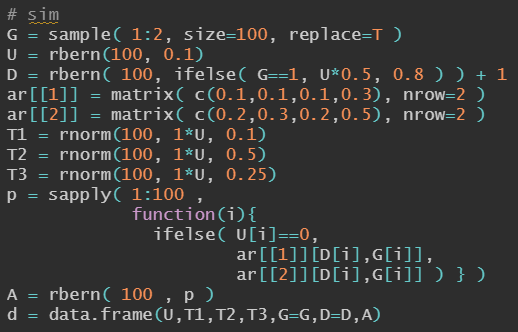
\includegraphics[scale=0.7]{descendant2_code.png}
				\caption*{(c) R code}
			\end{figure}
			%
		\end{column}
		%
		\begin{column}{0.5\textwidth}  
			%
			\begin{equ}
				%
				M = \left\{ \begin{aligned} 
					G \leftarrow & \; f_{G}(U_{G}) \\
					D \leftarrow & \; f_{D}(G,U_{X},U_{D}) \\
					A \leftarrow & \; f_{A}(D, G,U_{X},U_{A}) \\
					T_{i} \leftarrow & \; f_{T}(U_{X},U_{T}) \\
					U \sim & \; P(\pmb{U})
				\end{aligned} \right
				%
				\caption*{(a) structural model}
				%
			\end{equ}
			%
			\begin{figure}
				%
				\begin{tikzpicture}
					% nodes
					\node[formula] at (-2,0) {$U_{G}$};
					\node[formula] at (-1,-0.3) {$G$};
					\node[formula] at (-1,1) {$U_{D}$};
					\node[formula] at (0,1) {$D$};
					\node[formula] at (0.8,1) {$U_{X}$};
					\node[formula] at (2,-0.3) {$U_{A}$};
					\node[formula] at (1,-0.3) {$A$};
					\node[formula] at (2,0.3) {$T_{1}$};
					\node[formula] at (2,0.75) {$T_{2}$};
					\node[formula] at (2,1.2) {$T_{3}$};
					
					% paths
					\draw [{Circle [open]}-{latex}{Circle}](-1.7,0)--(-0.9,0); % Ug->G
					\draw [-{latex}](-0.9,0)--(0.9,0); % G->A
					\draw [{Circle [open]}-{latex}{Circle}](2,0)--(0.9,0); % Ua->A
					\draw [-{latex}](-0.95,0.05)--(0,0.75); % G->D
					\draw [{Circle [color=red]}-{latex}](0,0.8)--(0.9,0.1); % D->A
					\draw [{Circle[open]}-{latex}](-1,0.75)--(0,0.75); % Ud->D
					\draw [-{latex}](0.90,0.75)--(0.1,0.75); % Ux->D
					\draw [{Circle[open]}-{latex}](0.95,0.8)--(0.95,0.05); % Ux->A
					\draw [-{latex}{Circle}](1,0.75)--(1.7,0.3); % Ux->T1
					\draw [-{latex}{Circle}](1,0.75)--(1.7,0.75); % Ux->T2
					\draw [-{latex}{Circle}](1,0.75)--(1.7,1.2); % Ux->T3
					
					% extra
					\node at (0,-0.25) {$(?)$}; % symbol
				\end{tikzpicture}
				%
				\caption*{(b) causal diagram}
				%
			\end{figure}
			%
		\end{column}
		%
	\end{columns}
	%
\end{frame}
%
%
\begin{lhframe}[rhgraphic={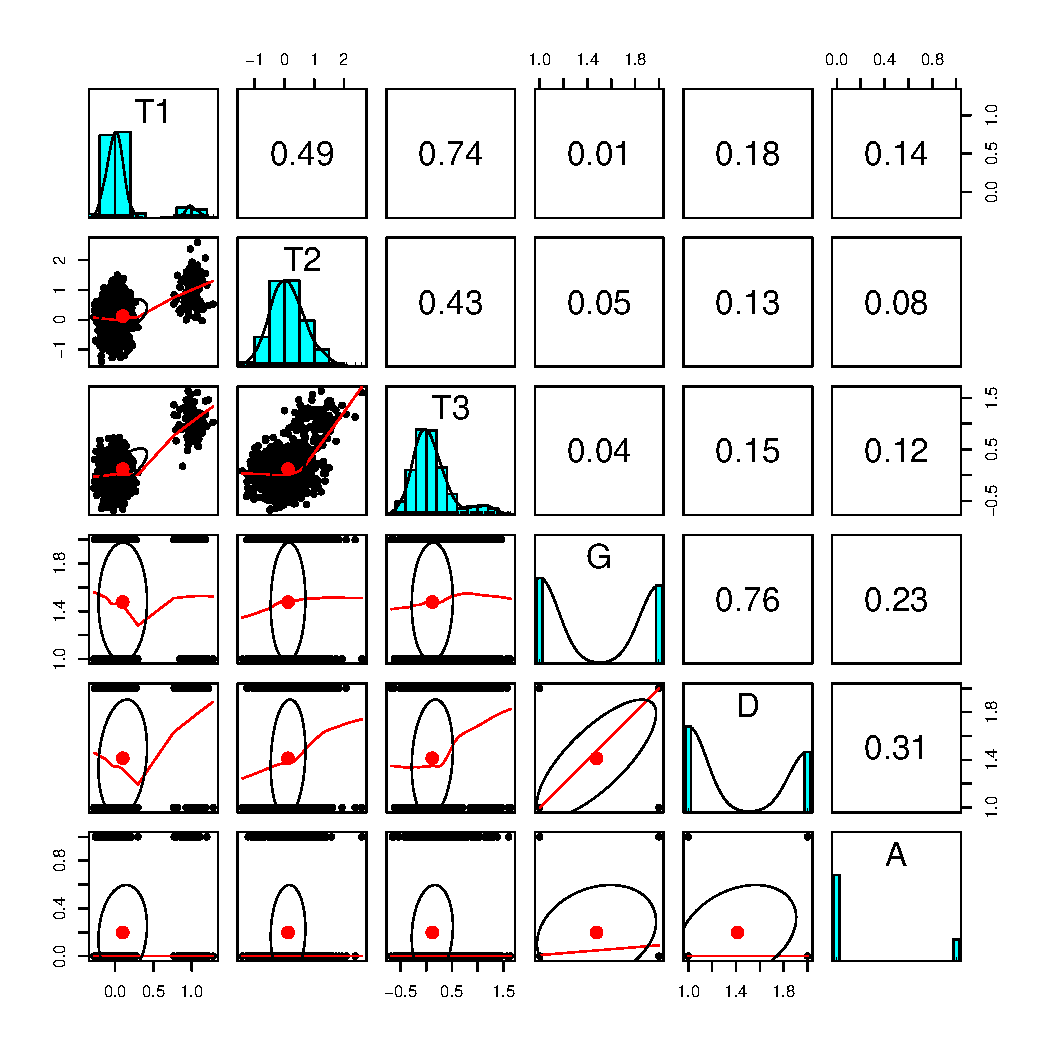
\includegraphics[scale=0.4]{descendant2_panel.pdf}}]
	{``Eyeballing" analysis}
	
	based on \textcolor{blue}{correlation analysis},
	%
	\begin{itemize}
		%
		\item the task has become more complex \\
		{\small (more variables to decide on)}
		%
		\item while $cor(H, I)>0$ indicate the more you work the more you gain \\
		{\small (but is it the only way?)}
		%
		\item since $cor(H, I)$ is high we \textcolor{blue}{might include it} as a covariate in our statistical model \\
		{\small (to improve the precision?)}
		%
	\end{itemize}
	%
\end{lhframe}
%
%
\begin{lhframe}[rhgraphic={\includegraphics[scale=0.3]{descendant2_reg.png}}]
	{Regression, regression!!}
	
	based on \textcolor{blue}{statistical analysis},
	%
	\begin{itemize}
		%
		\item we now have two models with two different ``levels" of effects
		\item which one is the ``truth"?
		%
	\end{itemize}
	%
\end{lhframe}
%
%
\begin{lhframe}[rhgraphic={\includegraphics[scale=0.45]{descendant2_samplesize.pdf}}]
	{The data tell-tell story!!}
	
	imagine we can continue sampling,
	%
	\begin{itemize}
		%
		\item top: $10,000$ samples $n=20$
		\item bottom: $10,000$ samples $n=100$
		%
	\end{itemize}
	
	under the \textcolor{blue}{incorrect model},\\
	the larger the sample size,
	%
	\begin{itemize}
		%
		\item the more \textcolor{blue}{certain} you are about your \textcolor{blue}{biased} estimates
		%
	\end{itemize}
	%
\end{lhframe}
%
%
\begin{frame}
	{So, what is going on?}
	%
	\begin{columns}
		%
		\begin{column}{0.5\textwidth}
			%
			based on \textcolor{blue}{DAG} and \textcolor{blue}{statistical model},
			%
			\begin{itemize}
				%
				\item stratifying on $I$ explains variability in $H$ (is his descendant) \\
				remaining variance is explained by $E$ \\
				{\small (big chunk is already explained)}
				%
				\item but there is more!!: \\
				$H$ is now a collider in the path $E \rightarrow H \leftarrow U_{H}$ \textcolor{blue}{(virtual collider)}, \\
				then, stratifying by $I$ \textcolor{blue}{opens that path} (biasing the estimates).
				%
			\end{itemize}
			%
		\end{column}
		%
		\begin{column}{0.5\textwidth}  
			%
			\begin{equ}
				%
				M = \left\{ \begin{aligned} 
					E \leftarrow & \; f_{E}(U_{E}) \\
					H \leftarrow & \; f_{H}(E,U_{H}) \\
					I \leftarrow & \; f_{I}(H,U_{I}) \\
					U \sim & \; P(\pmb{U})
				\end{aligned} \right
				%
				\caption*{(a) structural model}
				%
			\end{equ}
			%
			\begin{figure}
				%
				\begin{tikzpicture}
					% nodes
					\node[formula] at (-2,0) {$U_{E}$};
					\node[formula] at (-1,-0.3) {$E$};
					\node[formula] at (1,1.5) {$U_{I}$};
					\node[formula] at (0,1) {$I$};
					\node[formula] at (2,0) {$U_{H}$};
					\node[formula] at (1,-0.3) {$H$};
					
					% paths
					\draw [{Circle [open]}-{latex}{Circle}](-1.7,0)--(-0.9,0); % Ue->E
					\draw [-{latex}](-0.9,0)--(0.9,0); % E->H
					\draw [{Circle [open]}-{latex}{Circle}](1.7,0)--(0.9,0); % Uh->H
					\draw [-{latex}{Circle}](0.95,0.05)--(0,0.8); % H->I
					\draw [{Circle [open]}-{latex}](0.9,1.3)--(0.1,0.8); % Ui->I
					
					% extra
					\node at (0,-0.25) {$(?)$}; % symbol
				\end{tikzpicture}
				%
				\caption*{(b) causal diagram}
				%
			\end{figure}
			%
		\end{column}
		%
	\end{columns}
	%
\end{frame}
%
%
\begin{lhframe}[rhgraphic={\includegraphics[scale=0.5]{descendant2_reg1.png}}]
	{the dream team!!}
	
	based on \textcolor{blue}{DAG} and \textcolor{blue}{statistical analysis},
	%
	\begin{itemize}
		%
		\item the less biased model is the first, \\
		{\small \textcolor{blue}{(assuming our DAG is true)} }
		%
	\end{itemize}
	%
\end{lhframe}
%
%

\end{comment}

%%%%%%%%%%%%%%%%%%%%%%%%%%%%%%%%%%%%%%%%%%%%%%%%%%%%%%%%%%%
\subsection{Descendant: case control}
%%%%%%%%%%%%%%%%%%%%%%%%%%%%%%%%%%%%%%%%%%%%%%%%%%%%%%%%%%%
%
%
\begin{frame}[t, negative]
	\subsectionpage
\end{frame}
%
%
\begin{frame}
	{Case control\footnote{\citet{McElreath_2022}, lecture 6; \citet{Cinelli_et_al_2021} (p. 8, 19), \citet{Hernan_2020}, lesson 3}}
	%
	\begin{columns}
		%
		\begin{column}{0.5\textwidth}
			%
			also, 
			%
			\begin{itemize}
				%
				\item \textcolor{blue}{virtual collider}
				%
			\end{itemize}
			
			research question, 
			%
			\begin{itemize}
				%
				\item \textcolor{blue}{Does $E$ has a (direct) effect on $H$?}
				\item Should we include $I$ on our model?
				%
			\end{itemize}
			
			variables,
			%
			\begin{itemize}
				%
				\item E, education 
				\item H, hours in occupation \\
				{\small (standardized)}
				\item I, income
				%
			\end{itemize}
			%
		\end{column}
		%
		\begin{column}{0.5\textwidth}  
			%
			\begin{equ}
				%
				M = \left\{ \begin{aligned} 
					E \leftarrow & \; f_{E}(U_{E}) \\
					H \leftarrow & \; f_{H}(E,U_{H}) \\
					I \leftarrow & \; f_{I}(H,U_{I}) \\
					U \sim & \; P(\pmb{U})
				\end{aligned} \right
				%
				\caption*{(a) structural model}
				%
			\end{equ}
			%
			\begin{figure}
				%
				\begin{tikzpicture}
					% nodes
					\node[formula] at (-2,0) {$U_{E}$};
					\node[formula] at (-1,-0.3) {$E$};
					\node[formula] at (1,1.5) {$U_{I}$};
					\node[formula] at (0,1) {$I$};
					\node[formula] at (2,0) {$U_{H}$};
					\node[formula] at (1,-0.3) {$H$};
					
					% paths
					\draw [{Circle [open]}-{latex}{Circle}](-1.7,0)--(-0.9,0); % Ue->E
					\draw [-{latex}](-0.9,0)--(0.9,0); % E->H
					\draw [{Circle [open]}-{latex}{Circle}](1.7,0)--(0.9,0); % Uh->H
					\draw [-{latex}{Circle}](0.95,0.05)--(0,0.8); % H->I
					\draw [{Circle [open]}-{latex}](0.9,1.3)--(0.1,0.8); % Ui->I
					
					% extra
					\node at (0,-0.25) {$(?)$}; % symbol
				\end{tikzpicture}
				%
				\caption*{(b) causal diagram}
				%
			\end{figure}
			%
		\end{column}
		%
	\end{columns}
	%
\end{frame}
%
%
\begin{frame}
	{Simulation setting}
	%
	\begin{columns}
		%
		\begin{column}{0.5\textwidth}
			%
			\begin{figure}
				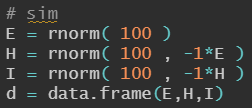
\includegraphics[scale=0.8]{descendant3_code.png}
				\caption*{(c) R code}
			\end{figure}
			%
			\textcolor{blue}{Implications},
			%
			\begin{itemize}
				\item \ndsep{E}{H} \\
				\item \dsep{E}{I} \; | H
				\item \ndsep{E}{$U_{H}$} \; | I \\
				{\small \textcolor{blue}{(virtual collider)} }
			\end{itemize}
			%
		\end{column}
		%
		\begin{column}{0.5\textwidth}  
			%
			\begin{equ}
				%
				M = \left\{ \begin{aligned} 
					E \leftarrow & \; f_{E}(U_{E}) \\
					H \leftarrow & \; f_{H}(E,U_{H}) \\
					I \leftarrow & \; f_{I}(H,U_{I}) \\
					U \sim & \; P(\pmb{U})
				\end{aligned} \right
				%
				\caption*{(a) structural model}
				%
			\end{equ}
			%
			\begin{figure}
				%
				\begin{tikzpicture}
					% nodes
					\node[formula] at (-2,0) {$U_{E}$};
					\node[formula] at (-1,-0.3) {$E$};
					\node[formula] at (1,1.5) {$U_{I}$};
					\node[formula] at (0,1) {$I$};
					\node[formula] at (2,0) {$U_{H}$};
					\node[formula] at (1,-0.3) {$H$};
					
					% paths
					\draw [{Circle [open]}-{latex}{Circle}](-1.7,0)--(-0.9,0); % Ue->E
					\draw [-{latex}](-0.9,0)--(0.9,0); % E->H
					\draw [{Circle [open]}-{latex}{Circle}](1.7,0)--(0.9,0); % Uh->H
					\draw [-{latex}{Circle}](0.95,0.05)--(0,0.8); % H->I
					\draw [{Circle [open]}-{latex}](0.9,1.3)--(0.1,0.8); % Ui->I
				\end{tikzpicture}
				%
				\caption*{(b) causal diagram}
				%
			\end{figure}
			%
		\end{column}
		%
	\end{columns}
	%
\end{frame}
%
%
\begin{lhframe}[rhgraphic={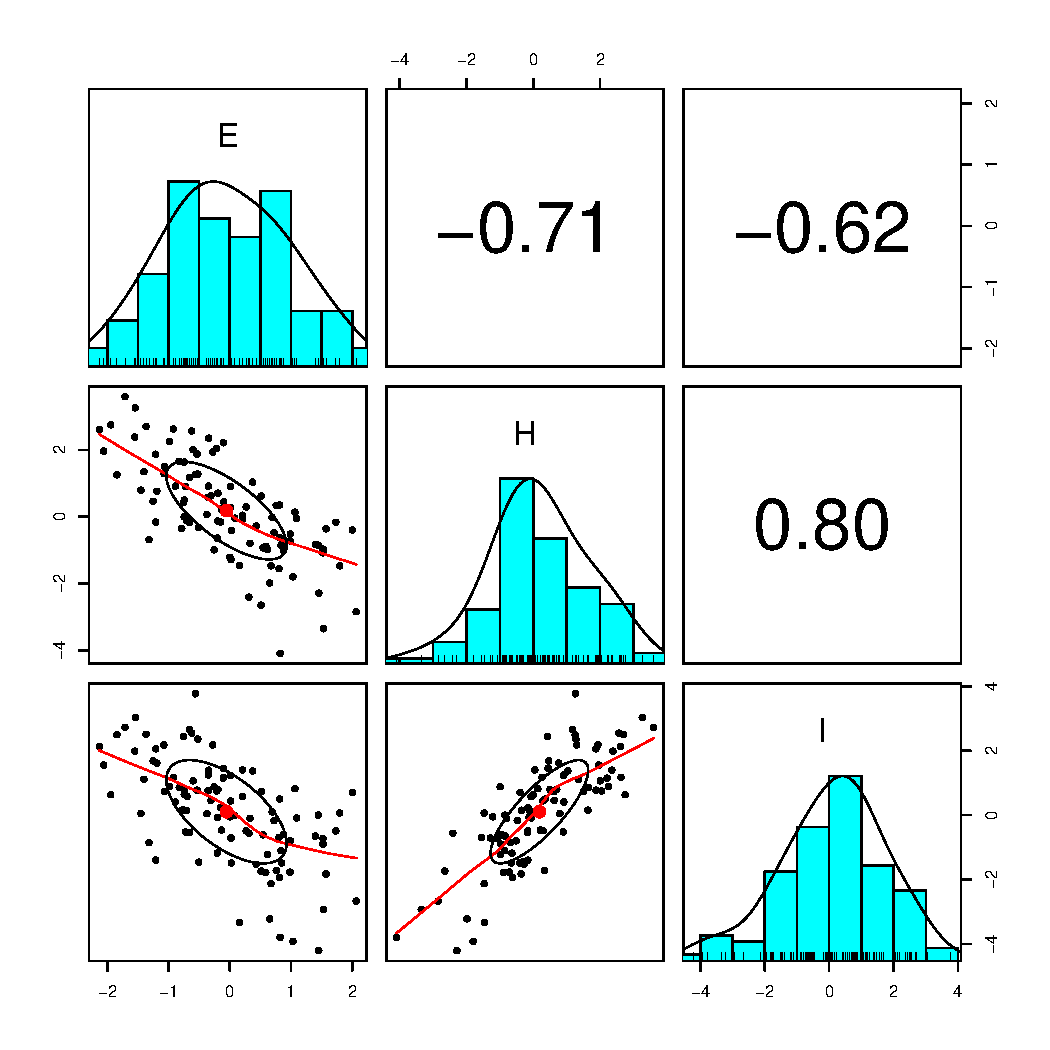
\includegraphics[scale=0.4]{descendant3_panel.pdf}}]
	{``Eyeballing" analysis}
	
	based on \textcolor{blue}{correlation analysis},
	%
	\begin{itemize}
		%
		\item $cor(E, I)<0$ does NOT goes in line of our ``rudimentary" understanding of the data.
		%
		\item while $cor(H, I)>0$ indicate the more you work the more you gain \\
		{\small (but is it the only way?)}
		%
		\item since $cor(H, I)$ is high we \textcolor{blue}{might include it} as a covariate in our statistical model \\
		{\small (to improve the precision?)}
		%
	\end{itemize}
	%
\end{lhframe}
%
%
\begin{lhframe}[rhgraphic={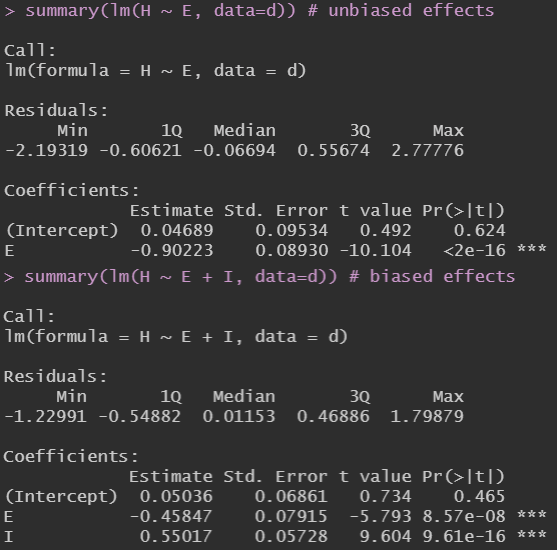
\includegraphics[scale=0.31]{descendant3_reg.png}}]
	{Regression, regression!!}
	
	based on \textcolor{blue}{statistical analysis},
	%
	\begin{itemize}
		%
		\item we now have two models with two different ``levels" of effects
		\item which one is the ``truth"?
		%
	\end{itemize}
	%
\end{lhframe}
%
%
\begin{lhframe}[rhgraphic={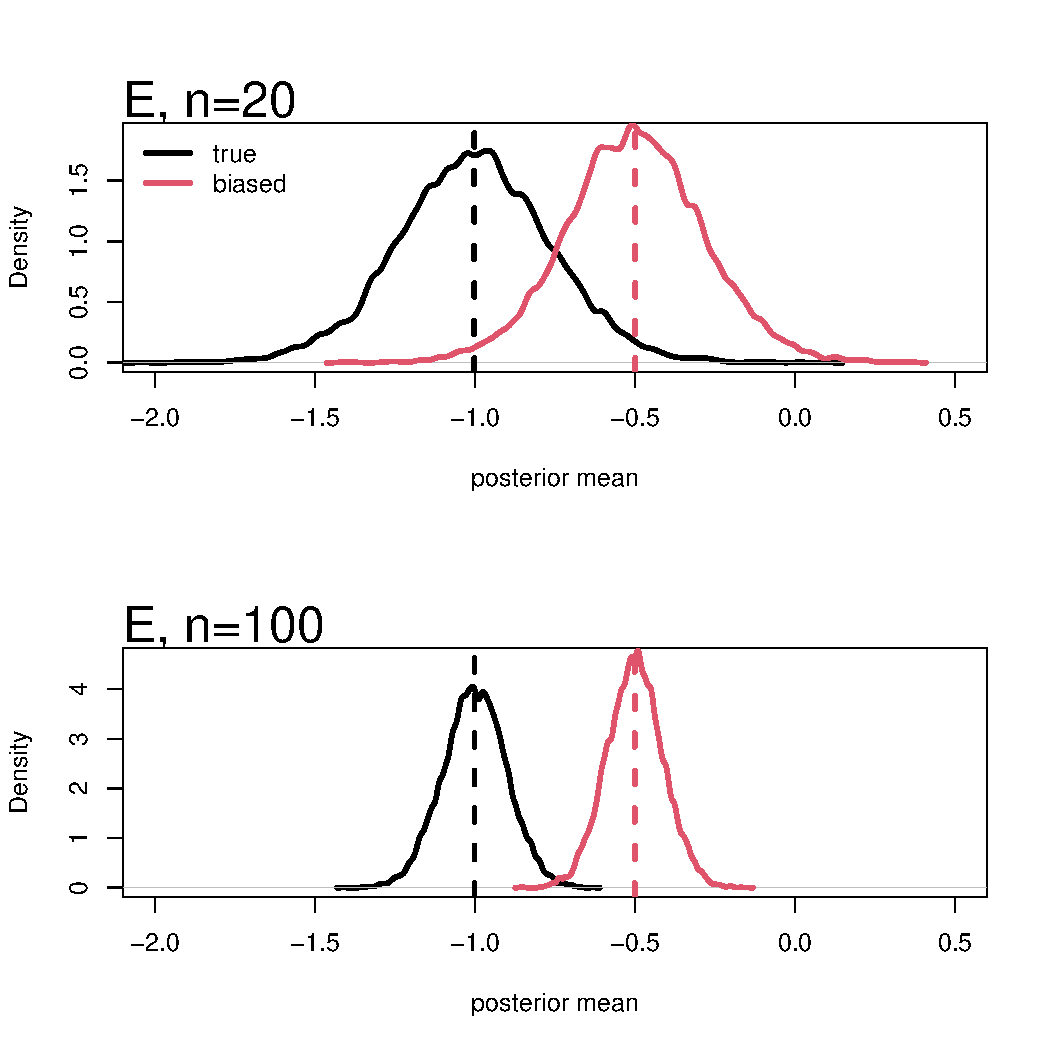
\includegraphics[scale=0.45]{descendant3_samplesize.pdf}}]
	{The data tell-tell story!!}
	
	imagine we can continue sampling,
	%
	\begin{itemize}
		%
		\item top: $10,000$ samples $n=20$
		\item bottom: $10,000$ samples $n=100$
		%
	\end{itemize}
	
	under the \textcolor{blue}{incorrect model},\\
	the larger the sample size,
	%
	\begin{itemize}
		%
		\item the more \textcolor{blue}{certain} you are about your \textcolor{blue}{biased} estimates
		%
	\end{itemize}
	%
\end{lhframe}
%
%
\begin{frame}
	{So, what is going on?}
	%
	\begin{columns}
		%
		\begin{column}{0.5\textwidth}
			%
			based on \textcolor{blue}{DAG} and \textcolor{blue}{statistical model},
			%
			\begin{itemize}
				%
				\item stratifying on $I$ explains variability in $H$ (is his descendant) \\
				remaining variance is explained by $E$ \\
				{\small (big chunk is already explained)}
				%
				\item but there is more!!: \\
				$H$ is now a collider in the path $E \rightarrow H \leftarrow U_{H}$ \textcolor{blue}{(virtual collider)}, \\
				then, stratifying by $I$ \textcolor{blue}{opens that path} (biasing the estimates).
				%
			\end{itemize}
			%
		\end{column}
		%
		\begin{column}{0.5\textwidth}  
			%
			\begin{equ}
				%
				M = \left\{ \begin{aligned} 
					E \leftarrow & \; f_{E}(U_{E}) \\
					H \leftarrow & \; f_{H}(E,U_{H}) \\
					I \leftarrow & \; f_{I}(H,U_{I}) \\
					U \sim & \; P(\pmb{U})
				\end{aligned} \right
				%
				\caption*{(a) structural model}
				%
			\end{equ}
			%
			\begin{figure}
				%
				\begin{tikzpicture}
					% nodes
					\node[formula] at (-2,0) {$U_{E}$};
					\node[formula] at (-1,-0.3) {$E$};
					\node[formula] at (1,1.5) {$U_{I}$};
					\node[formula] at (0,1) {$I$};
					\node[formula] at (2,0) {$U_{H}$};
					\node[formula] at (1,-0.3) {$H$};
					
					% paths
					\draw [{Circle [open]}-{latex}{Circle}](-1.7,0)--(-0.9,0); % Ue->E
					\draw [-{latex}](-0.9,0)--(0.9,0); % E->H
					\draw [{Circle [open]}-{latex}{Circle}](1.7,0)--(0.9,0); % Uh->H
					\draw [-{latex}{Circle}](0.95,0.05)--(0,0.8); % H->I
					\draw [{Circle [open]}-{latex}](0.9,1.3)--(0.1,0.8); % Ui->I
					
					% extra
					\node at (0,-0.25) {$(?)$}; % symbol
				\end{tikzpicture}
				%
				\caption*{(b) causal diagram}
				%
			\end{figure}
			%
		\end{column}
		%
	\end{columns}
	%
\end{frame}
%
%
\begin{lhframe}[rhgraphic={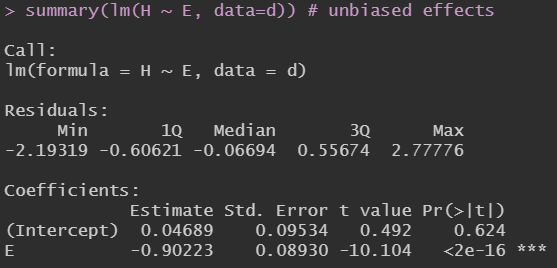
\includegraphics[scale=0.52]{descendant3_reg1.png}}]
	{the dream team!!}
	
	based on \textcolor{blue}{DAG} and \textcolor{blue}{statistical analysis},
	%
	\begin{itemize}
		%
		\item the less biased model is the first, \\
		{\small \textcolor{blue}{(assuming our DAG is true)} }
		%
	\end{itemize}
	%
\end{lhframe}
%
%
\begin{frame}
	{Similar, but different\footnote{\citet{Cinelli_et_al_2021} (p. 7)}}
	%
	\begin{columns}
		%
		\begin{column}{0.5\textwidth}
			%
			research question, 
			%
			\begin{itemize}
				%
				\item \textcolor{blue}{What is the effect of $X$ on $Y$?}
				\item Should we include $Z$ in the model?
				%
			\end{itemize}
			
			variables,
			%
			\begin{itemize}
				%
				\item Z, ``child" of X
				\item X, exposure
				\item Y, outcome
				%
			\end{itemize}
			%
		\end{column}
		%
		\begin{column}{0.5\textwidth}  
			%
			\begin{equ}
				%
				M = \left\{ \begin{aligned} 
					X \leftarrow & \; f_{X}(U_{X}) \\
					Z \leftarrow & \; f_{Z}(X, U_{Z}) \\
					Y \leftarrow & \; f_{Y}(X, U_{Y}) \\
					U \sim & \; P(\pmb{U})
				\end{aligned} \right
				%
				\caption*{(a) structural model}
				%
			\end{equ}
			%
			\begin{figure}
				%
				\begin{tikzpicture}
					% nodes
					\node[formula] at (-2,0.8) {$U_{Z}$};
					\node[formula] at (-1,1) {$Z$};
					\node[formula] at (-2,0) {$U_{X}$};
					\node[formula] at (-1,-0.3) {$X$};
					\node[formula] at (1,-0.3) {$Y$};
					\node[formula] at (2,0) {$U_{Y}$};
					
					% paths
					\draw [{Circle [open]}-{latex}{Circle}](-1.7,0.75)--(-0.9,0.75); % Uz->Z
					\draw [-{latex}](-0.95,0.05)--(-0.95,0.70); % X->Z
					\draw [{Circle [open]}-{latex}{Circle}](-1.7,0)--(-0.9,0); % Ux->X
					\draw [-{latex}](-0.9,0)--(0.9,0); % X->Y
					\draw [{Circle [open]}-{latex}{Circle}](1.7,0)--(0.9,0); % Uy->Y
					
					% extra
					\node at (0,-0.25) {$(?)$}; % symbol
				\end{tikzpicture}
				%
				\caption*{(b) causal diagram}
				%
			\end{figure}
			%
		\end{column}
		%
	\end{columns}
	%
\end{frame}
%
%
\begin{lhframe}[rhgraphic={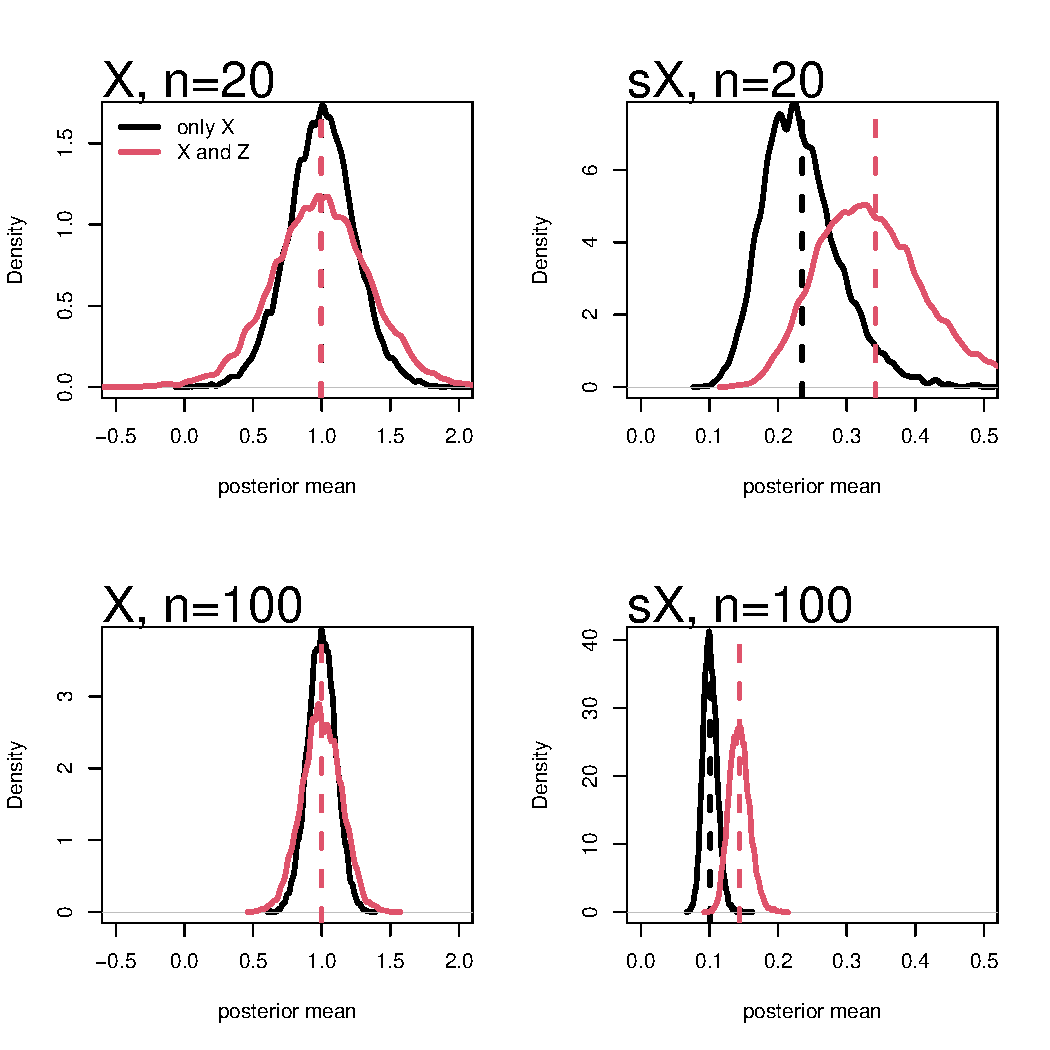
\includegraphics[scale=0.45]{descendant3b_samplesize.pdf}}]
	{Similar, but different}
	
	imagine we can continue sampling,
	%
	\begin{itemize}
		%
		\item top: $10,000$ samples $n=20$
		\item bottom: $10,000$ samples $n=100$
		%
	\end{itemize}
	
	under the \textcolor{blue}{incorrect model},\\
	the larger the sample size,
	%
	\begin{itemize}
		%
		\item you loose \textcolor{blue}{certainty} in your \textcolor{blue}{non-biased} estimates
		%
	\end{itemize}
	%
\end{lhframe}
%
%
%%%%%%%%%%%%%%%%%%%%%%%%%%%%%%%%%%%%%%%%%%%%%%%%%%%%%%%%%%%
\subsection{Descendant: measurement error, outcome only}
%%%%%%%%%%%%%%%%%%%%%%%%%%%%%%%%%%%%%%%%%%%%%%%%%%%%%%%%%%%
%
%
\begin{frame}[t, negative]
	\subsectionpage
\end{frame}
%
%
\begin{frame}
	{Measurement error, outcome only\footnote{\citet{McElreath_2020}, chapter 15 (p. 491)}}
	%
	\begin{columns}
		%
		\begin{column}{0.5\textwidth}
			%
			also, 
			%
			\begin{itemize}
				%
				\item \textcolor{blue}{residual confounding}
				\item think \textcolor{blue}{meta analysis} or \textcolor{blue}{clustering}
				%
			\end{itemize}
			
			research question, 
			%
			\begin{itemize}
				%
				\item \textcolor{blue}{Does $M$ has a (direct) effect on $D$?}
				%
			\end{itemize}
			
			variables,
			%
			\begin{itemize}
				%
				\item A, median age at marriage
				\item M, marriage rate
				\item Dt, divorce rate (\textit{true} rate)
				\item Do, divorce rate (\textit{observed} rate)
				%
			\end{itemize}
			%
			
			extras,
			%
			\begin{itemize}
				%
				\item $U_{D}$, between variability (\textit{true} rate)
				\item $U_{O}$, measurement error
				%
			\end{itemize}
			%
		\end{column}
		%
		\begin{column}{0.5\textwidth}  
			%
			\begin{equ}
				%
				M = \left\{ \begin{aligned} 
				A \leftarrow & \; f_{A}(U_{A}) \\
				M \leftarrow & \; f_{M}(A,U_{M}) \\
				Dt \leftarrow & \; f_{D}(A, M, U_{D}) \\
				Do \leftarrow & \; f_{D}(Dt, U_{O}) \\
				U \sim & \; P(\pmb{U})
				%
			\end{aligned} \right
			%
			\caption*{(a) structural model}
			%
			\end{equ}
			%
			\begin{figure}
				%
				\begin{tikzpicture}
					% nodes
					\node[formula] at (-2,0) {$U_{M}$};
					\node[formula] at (-1,-0.3) {$M$};
					\node[formula] at (1,1.5) {$U_{A}$};
					\node[formula] at (0,1) {$A$};
					\node[formula] at (1.8,0.7) {$U_{D}$};
					\node[formula] at (1,-0.3) {$Dt$};
					\node[formula] at (2.7,0.7) {$U_{O}$};
					\node[formula] at (1.95,-0.3) {$Do$};
		
					% paths
					\draw [{Circle [open]}-{latex}{Circle}](-1.7,0)--(-0.9,0); % Um->M
					\draw [-{latex}](-0.9,0)--(0.9,0); % M->Dt
					\draw [{Circle [open]}-{latex}{Circle}](0.9,0)--(2,0); % Dt->Do
					\draw [{Circle [open]}-{latex}](1.7,0.5)--(1.05,0.05); % Ud->Dt
					\draw [{Circle [open]}-{latex}](2.6,0.5)--(2,0.05); % Uo->Do
					\draw [{Circle [color=red]}-{latex}](0.1,0.8)--(-0.9,0.1); % A->M
					\draw [-{latex}](0.1,0.75)--(0.9,0.1); % A->D
					\draw [{Circle [open]}-{latex}](0.9,1.3)--(0.1,0.8); % Ua->A
		
					% extra
					\node at (0,-0.25) {$(?)$}; % symbol
				\end{tikzpicture}
				%
				\caption*{(b) causal diagram}
				%
			\end{figure}
			%
		\end{column}
		%
	\end{columns}
	%
\end{frame}
%
%
\begin{frame}
	{Simulation setting}
	%
	\begin{columns}
		%
		\begin{column}{0.5\textwidth}
			%
			\begin{figure}
				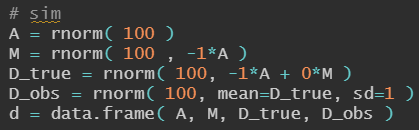
\includegraphics[scale=0.8]{descendant4_code.png}
				\caption*{(c) R code}
			\end{figure}
			%
			\textcolor{blue}{Implications},
			%
			\begin{itemize}
				\item \ndsep{M}{Dt} \\
				\item \ndsep{M}{Do} \\
				\item \dsep{M}{Dt} \; | A {\small (not possible)}
				\item \dsep{M}{Do} \; | A
			\end{itemize}
			%
		\end{column}
		%
		\begin{column}{0.5\textwidth}  
			%
			\begin{equ}
				%
				M = \left\{ \begin{aligned} 
					A \leftarrow & \; f_{A}(U_{A}) \\
					M \leftarrow & \; f_{M}(A,U_{M}) \\
					Dt \leftarrow & \; f_{D}(A, U_{D}) \\
					Do \leftarrow & \; f_{D}(Dt, U_{O}) \\
					U \sim & \; P(\pmb{U})
					%
				\end{aligned} \right
				%
				\caption*{(a) structural model}
				%
			\end{equ}
			%
			\begin{figure}
				%
				\begin{tikzpicture}
					% nodes
					\node[formula] at (-2,0) {$U_{M}$};
					\node[formula] at (-1,-0.3) {$M$};
					\node[formula] at (1,1.5) {$U_{A}$};
					\node[formula] at (0,1) {$A$};
					\node[formula] at (1.8,0.7) {$U_{D}$};
					\node[formula] at (1,-0.3) {$Dt$};
					\node[formula] at (2.7,0.7) {$U_{O}$};
					\node[formula] at (1.95,-0.3) {$Do$};
					
					% paths
					\draw [{Circle [open]}-{latex}{Circle}](-1.7,0)--(-0.9,0); % Um->M
					%\draw [-{latex}](-0.9,0)--(0.9,0); % M->Dt
					\draw [{Circle [open]}-{latex}{Circle}](0.9,0)--(2,0); % Dt->Do
					\draw [{Circle [open]}-{latex}](1.7,0.5)--(1.05,0.05); % Ud->Dt
					\draw [{Circle [open]}-{latex}](2.6,0.5)--(2,0.05); % Uo->Do
					\draw [{Circle [color=red]}-{latex}](0.1,0.8)--(-0.9,0.1); % A->M
					\draw [-{latex}](0.1,0.75)--(0.9,0.1); % A->D
					\draw [{Circle [open]}-{latex}](0.9,1.3)--(0.1,0.8); % Ua->A
					%
				\end{tikzpicture}
				%
				\caption*{(b) causal diagram}
				%
			\end{figure}
			%
		\end{column}
		%
	\end{columns}
	%
\end{frame}
%
%
\begin{frame}
	{So, what does the simulation means?}
	
	\begin{figure*}
		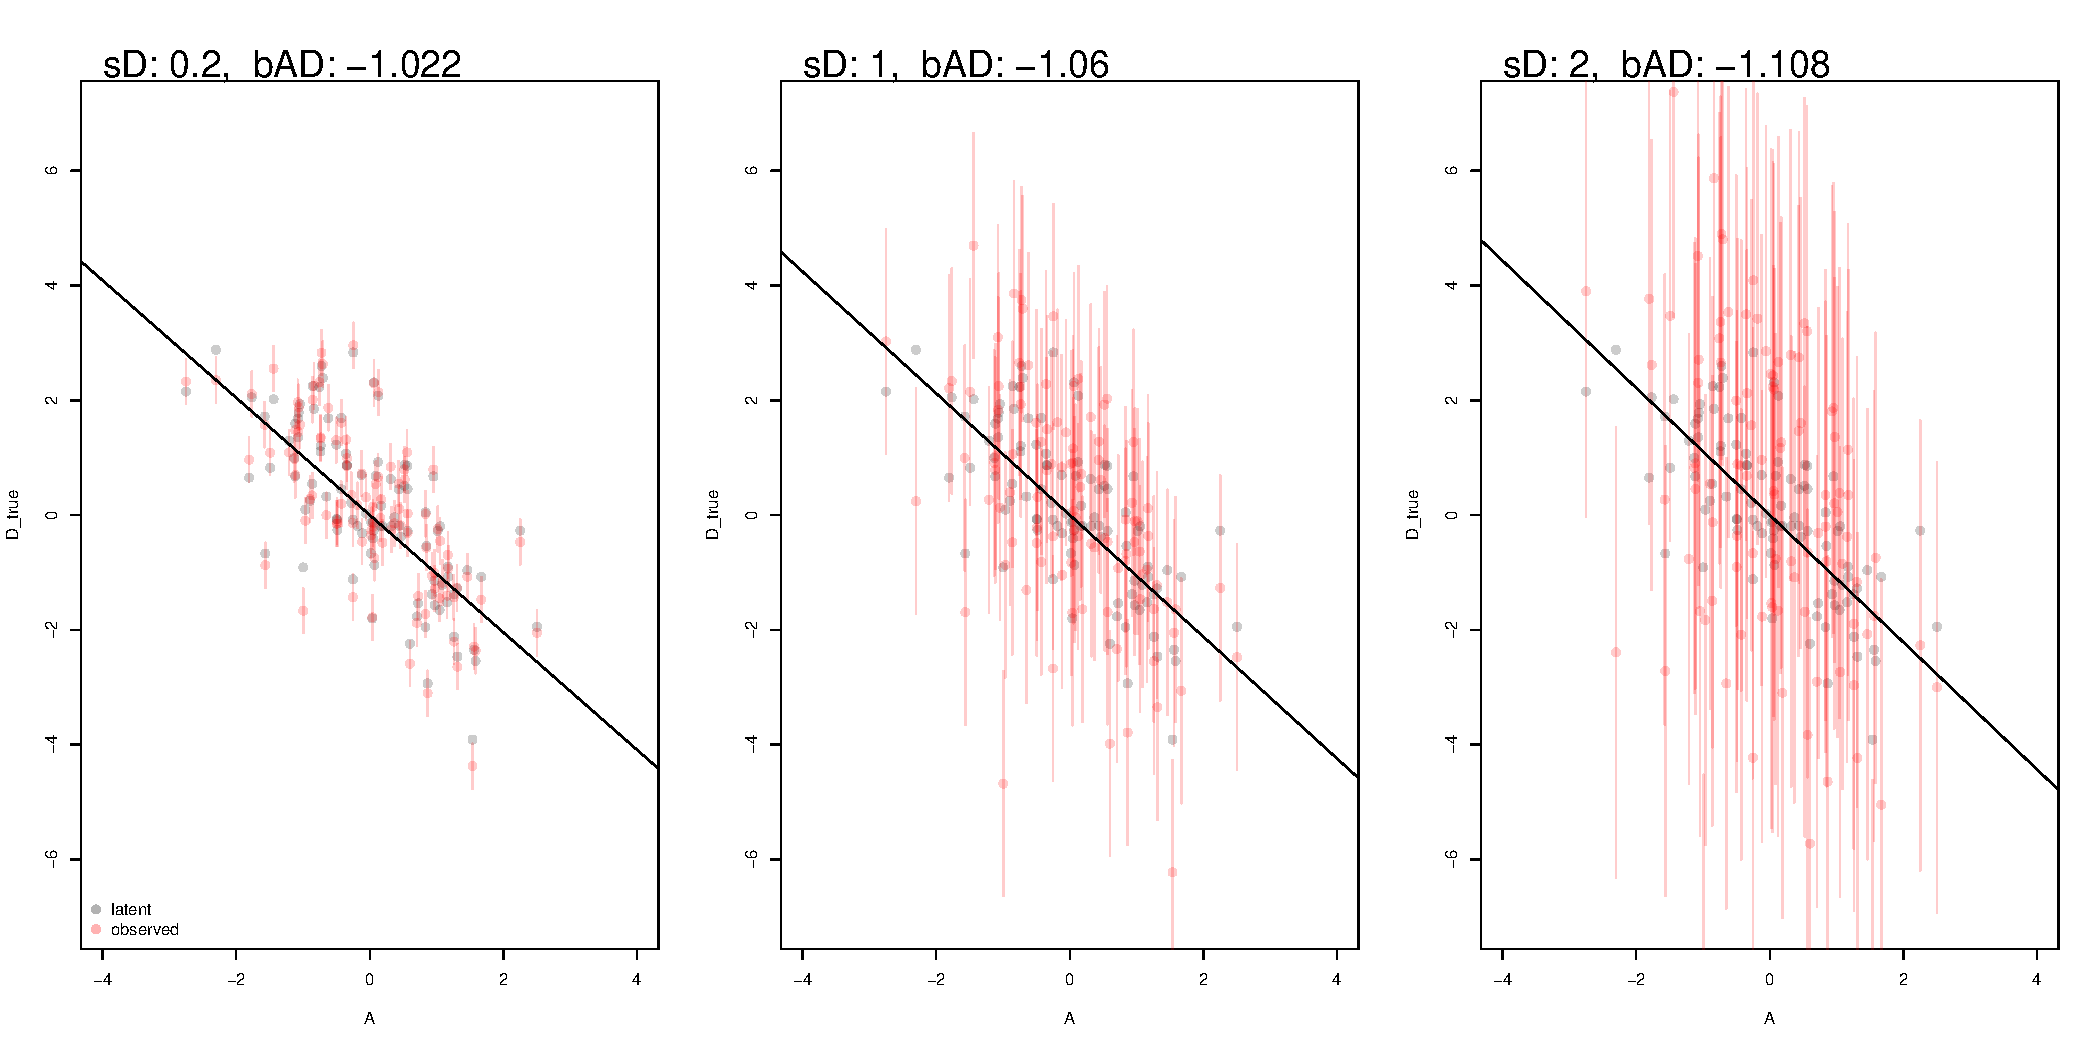
\includegraphics[width=\linewidth]{descendant4_me1.pdf}
	\end{figure*}
	%
\end{frame}
%
%
\begin{frame}
	{So, what does the simulation means?}
	
	\begin{figure*}
		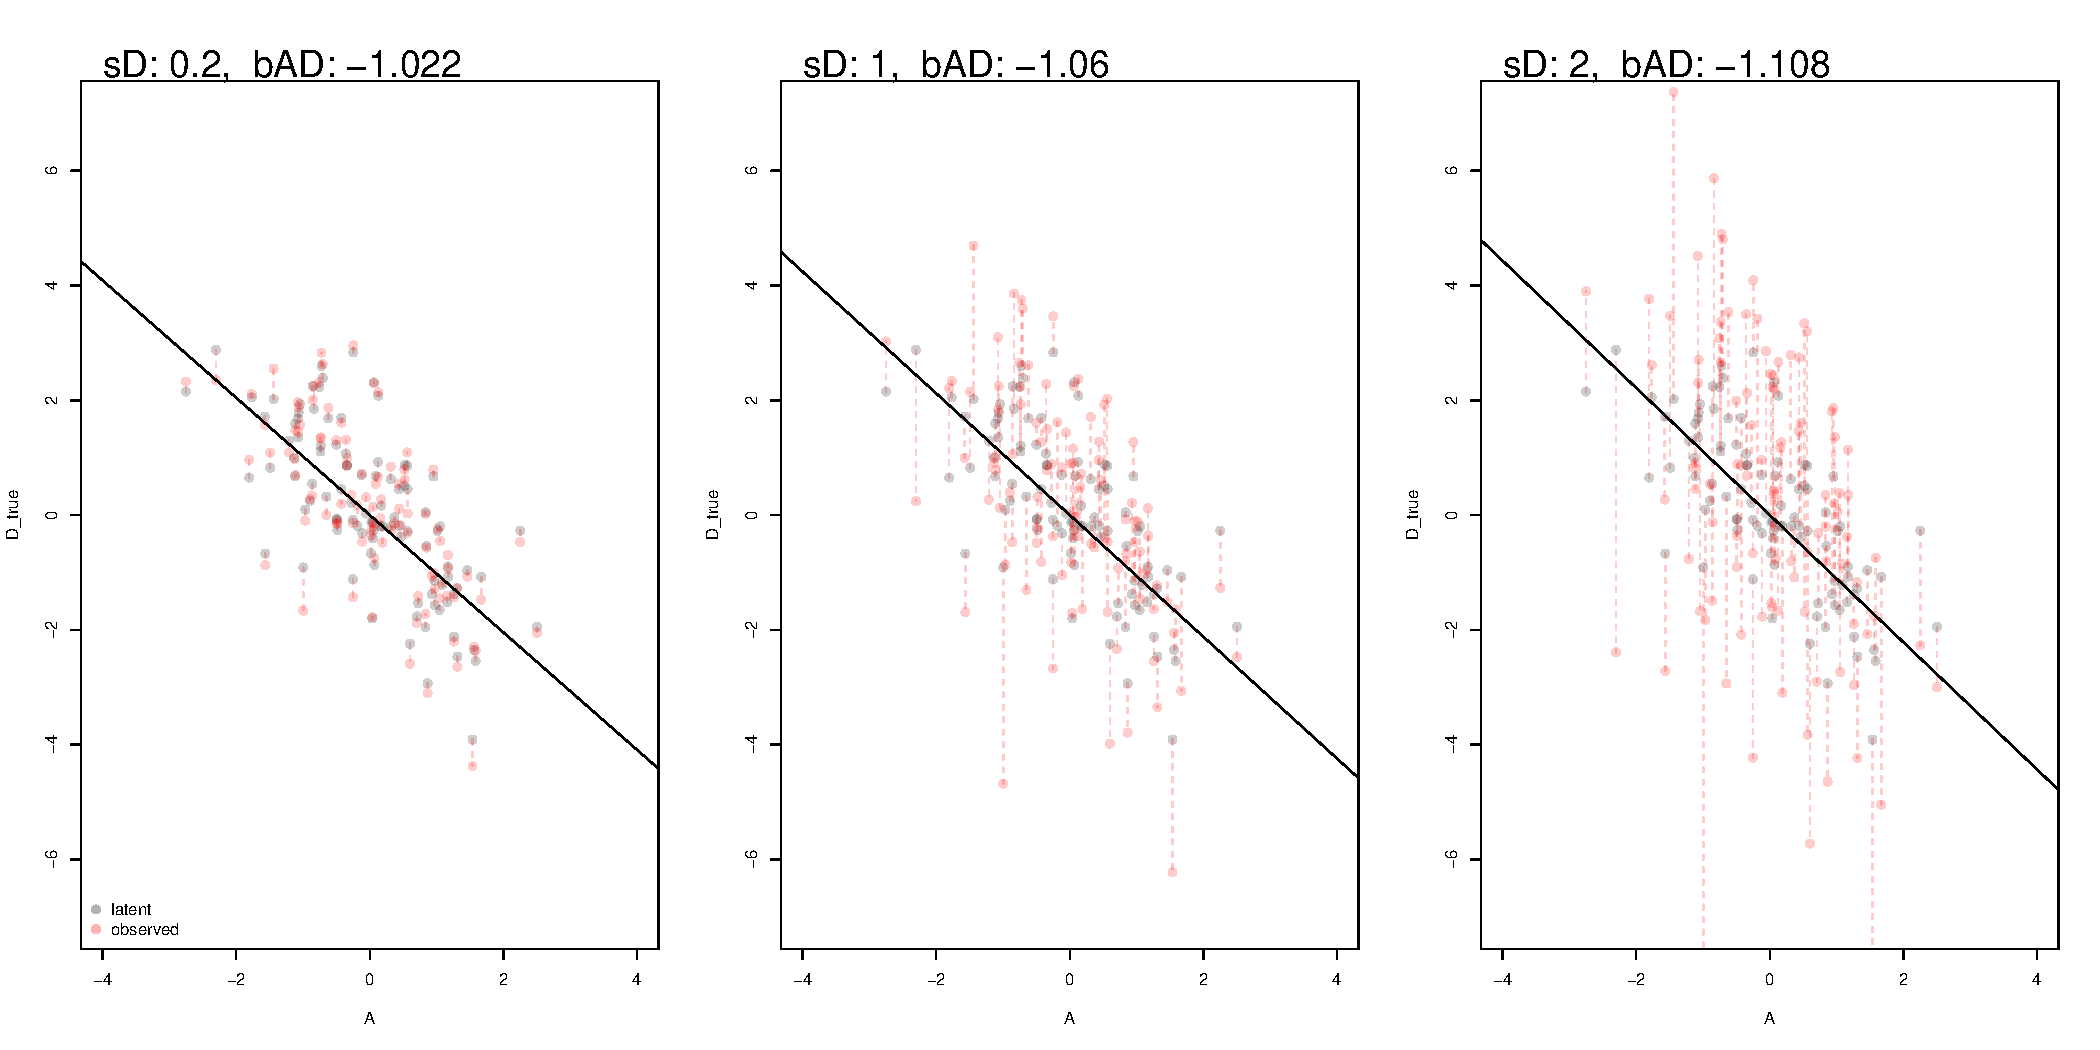
\includegraphics[width=\linewidth]{descendant4_me2.pdf}
	\end{figure*}
	%
\end{frame}
%
%
\begin{lhframe}[rhgraphic={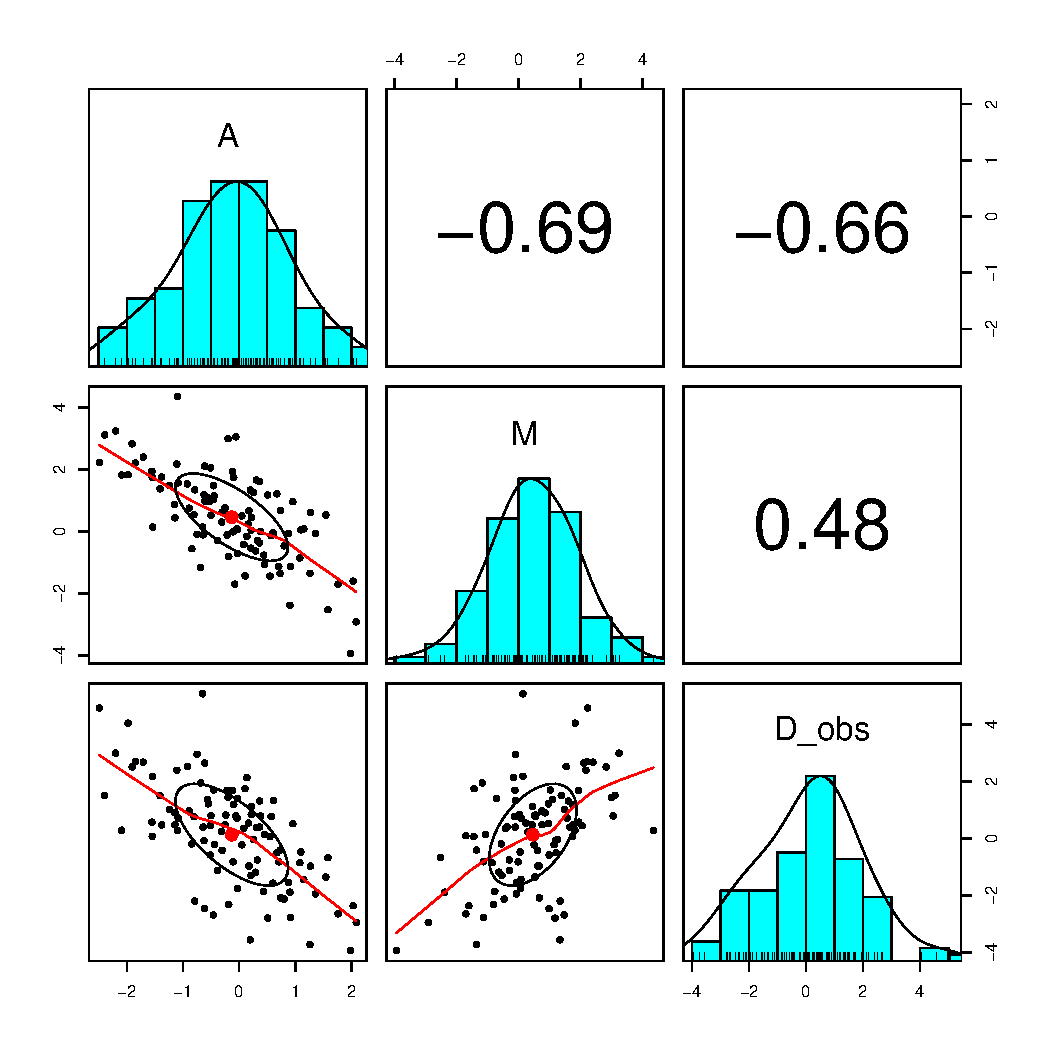
\includegraphics[scale=0.4]{descendant4_panel.pdf}}]
	{``Eyeballing" analysis}
	
	based on \textcolor{blue}{correlation analysis},
	%
	\begin{itemize}
		%
		\item $cor(A, D_{obs})<0$ and $cor(M, D_{obs})>0$
		goes in line of our ``rudimentary" understanding of the data.
		%
		\item why there is $cor(M, D_{obs})>0$? \\
		{\small (hint: univariate correlation)}
		%
		\item we \textcolor{blue}{include} $M$ as a covariate in our statistical model \\
		{\small (besides, it is our research hypothesis)}
		%
	\end{itemize}
	%
\end{lhframe}
%
%
\begin{lhframe}[rhgraphic={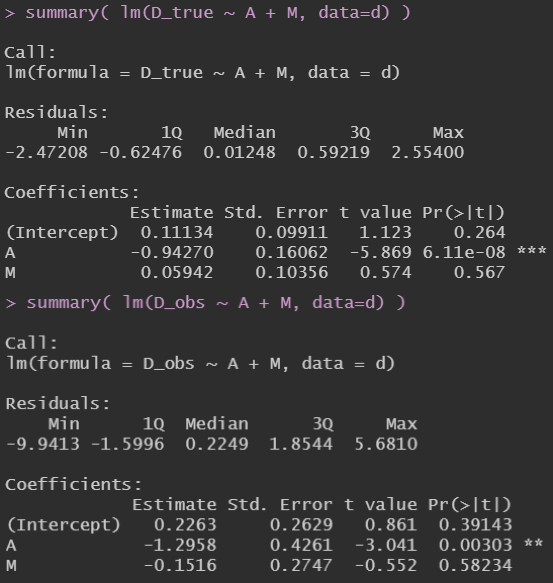
\includegraphics[scale=0.3]{descendant4_reg.png}}]
	{Regression, regression!!}
	
	based on \textcolor{blue}{statistical analysis},
	%
	\begin{itemize}
		%
		\item first model is impossible (\textcolor{blue}{unobservable})
		\item no effect bias in \textcolor{blue}{observable} data
		\item we have \textcolor{blue}{larger} standard error \\
		{\small (in this case does not change the hypothesis, but with smaller effects it could happen)}
		%
	\end{itemize}
	%
\end{lhframe}
%
%
\begin{lhframe}[rhgraphic={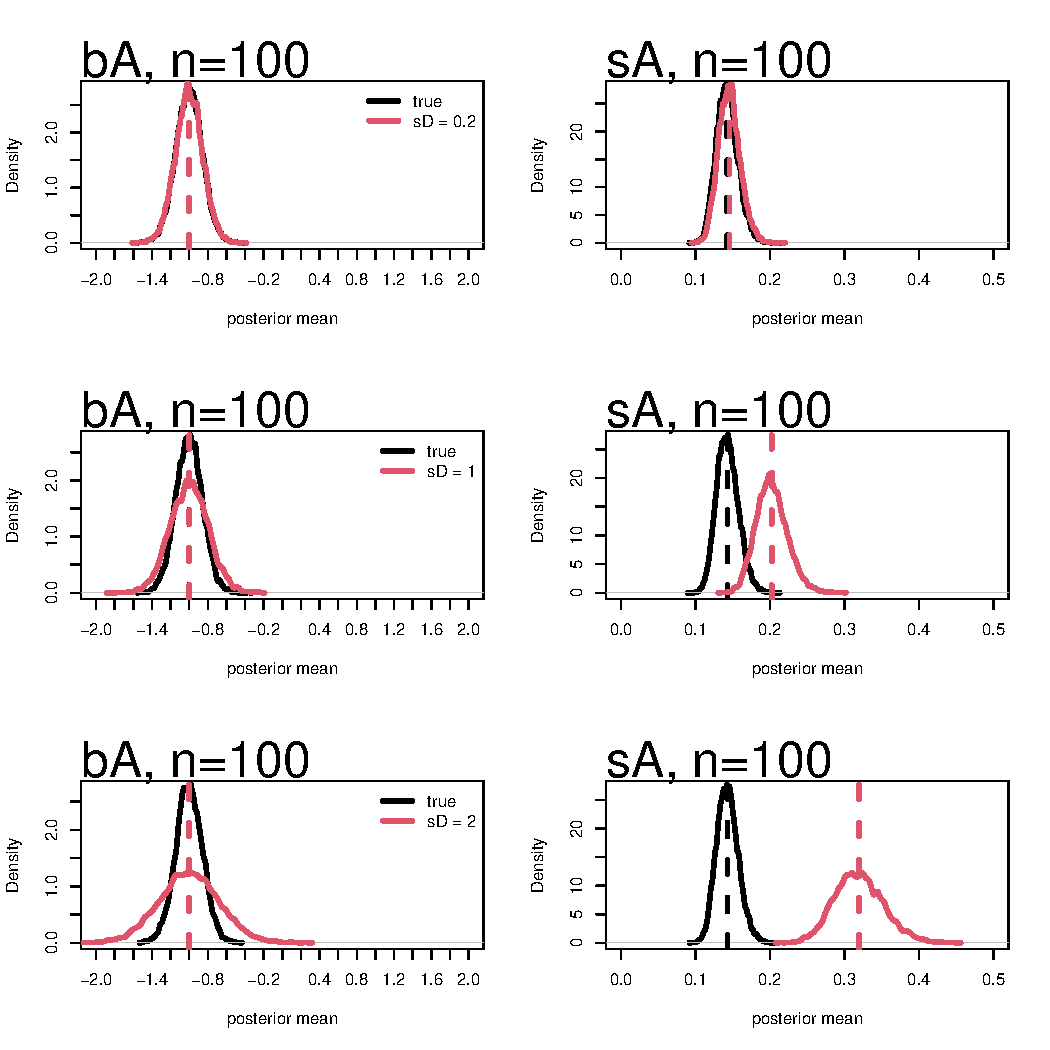
\includegraphics[scale=0.45]{descendant4_samplesize.pdf}}]
	{So, what is going on?}
	
	imagine we can continue sampling,
	%
	\begin{itemize}
		%
		\item $10,000$ samples $n=100$
		%
	\end{itemize}
	
	notice,
	%
	\begin{itemize}
		%
		\item the larger the \textcolor{blue}{measurement error}, the \textcolor{blue}{less confident} you are of your estimates,
		%
		\item larger \textcolor{blue}{measurement error} (in outcomes) \textcolor{blue}{does not bias} the effects, 
		%
	\end{itemize}
	%
\end{lhframe}
%
%
\begin{frame}
	{How can I fix it???}
	%
	\begin{columns}
		%
		\begin{column}{0.5\textwidth}
			%
			\begin{equ}
				%
				\begin{aligned} 
					D_{obs} \sim & \; N( D_{true}, \sigma_{O}) \\
					D_{true} \sim & \; N( \mu, \sigma_{D}) \\
					\mu = & \; \alpha + \beta_{AD} A + \beta_{MD} M
				\end{aligned}
				%
				\caption*{(c) probabilistic model}
				%
			\end{equ}
			%
			based on \textcolor{blue}{DAG} and \textcolor{blue}{statistical model}, \\
			use the knowledge of the system
			%
			\begin{itemize}
				%
				\item measurement error part: $D_{obs} \sim N( D_{true}, \sigma_{O})$, 
				%
				\item latent structure: $D_{true} \sim N( \mu, \sigma_{D} )$,
				%
				\item latent regression: $\mu = f(A, M)$
				%
			\end{itemize}
			%
		\end{column}
		%
		\begin{column}{0.5\textwidth}  
			%
			\begin{equ}
				%
				M = \left\{ \begin{aligned} 
					A \leftarrow & \; f_{A}(U_{A}) \\
					M \leftarrow & \; f_{M}(A,U_{M}) \\
					Dt \leftarrow & \; f_{D}(A, M, U_{D}) \\
					Do \leftarrow & \; f_{D}(Dt, U_{O}) \\
					U \sim & \; P(\pmb{U})
					%
				\end{aligned} \right
				%
				\caption*{(a) structural model}
				%
			\end{equ}
			%
			\begin{figure}
				%
				\begin{tikzpicture}
					% nodes
					\node[formula] at (-2,0) {$U_{M}$};
					\node[formula] at (-1,-0.3) {$M$};
					\node[formula] at (1,1.5) {$U_{A}$};
					\node[formula] at (0,1) {$A$};
					\node[formula] at (1.8,0.7) {$U_{D}$};
					\node[formula] at (1,-0.3) {$Dt$};
					\node[formula] at (2.7,0.7) {$U_{O}$};
					\node[formula] at (1.95,-0.3) {$Do$};
					
					% paths
					\draw [{Circle [open]}-{latex}{Circle}](-1.7,0)--(-0.9,0); % Um->M
					\draw [-{latex}](-0.9,0)--(0.9,0); % M->Dt
					\draw [{Circle [open]}-{latex}{Circle}](0.9,0)--(2,0); % Dt->Do
					\draw [{Circle [open]}-{latex}](1.7,0.5)--(1.05,0.05); % Ud->Dt
					\draw [{Circle [open]}-{latex}](2.6,0.5)--(2,0.05); % Uo->Do
					\draw [{Circle [color=red]}-{latex}](0.1,0.8)--(-0.9,0.1); % A->M
					\draw [-{latex}](0.1,0.75)--(0.9,0.1); % A->D
					\draw [{Circle [open]}-{latex}](0.9,1.3)--(0.1,0.8); % Ua->A
					
					% extra
					\node at (0,-0.25) {$(?)$}; % symbol
				\end{tikzpicture}
				%
				\caption*{(b) causal diagram}
				%
			\end{figure}
			%
		\end{column}
		%
	\end{columns}
	%
\end{frame}
%
%
\begin{lhframe}[rhgraphic={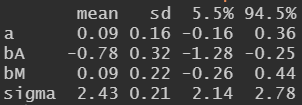
\includegraphics[scale=0.8]{descendant4_reg3.png}}]
	{How can I fix it???}
	
	\begin{figure}
		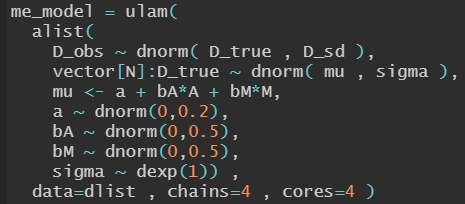
\includegraphics[scale=0.7]{descendant4_code2.png}
	\end{figure}
	%
	
	Using \textcolor{blue}{DAG} and \textcolor{blue}{Bayesian} analysis:
	%
	\begin{itemize}
		%
		\item measurement error part: $D_{obs} \sim N( D_{true}, S_{obs})$, 
		%
		\item latent structure: $D_{true} \sim N( \mu, \sigma )$,
		%
		\item latent regression: $\mu = f(A, M)$
		%
	\end{itemize}
	%
\end{lhframe}
%
%
\begin{lhframe}[rhgraphic={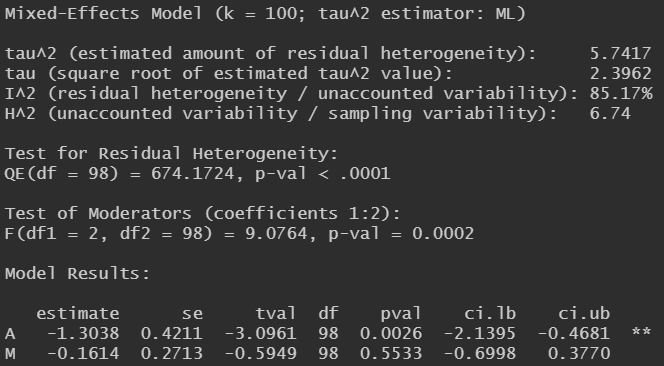
\includegraphics[scale=0.42]{descendant4_reg4.png}}]
	{How can I fix it???}
	
	\begin{figure}
		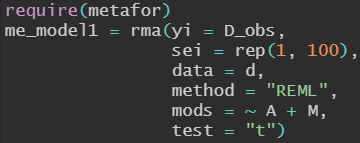
\includegraphics[scale=0.7]{descendant4_code3.png}
	\end{figure}
	%
	
	Using \textcolor{blue}{DAG} and \textcolor{blue}{frequentist} analysis:
	%
	\begin{itemize}
		%
		\item measurement error part: $D_{obs} = \mu + \delta + \epsilon$, 
		%
		\item 2-level variability: $\delta \sim N(0, \tau)$,
		%
		\item residual variability: $\epsilon \sim N(0, \sigma_{\epsilon})$,
		%
		\item 2-level regression: $\mu = f(A, M)$
		%
	\end{itemize}
	%
\end{lhframe}
%
%
%%%%%%%%%%%%%%%%%%%%%%%%%%%%%%%%%%%%%%%%%%%%%%%%%%%%%%%%%%%
\subsection{Descendant: measurement error, predictor only}
%%%%%%%%%%%%%%%%%%%%%%%%%%%%%%%%%%%%%%%%%%%%%%%%%%%%%%%%%%%
%
%
\begin{frame}[t, negative]
	\subsectionpage
\end{frame}
%
%
\begin{frame}
	{Measurement error, predictor only\footnote{\citet{McElreath_2020}, chapter 15 (p. 495)}}
	%
	\begin{columns}
		%
		\begin{column}{0.5\textwidth}
			%
			also, 
			%
			\begin{itemize}
				%
				\item \textcolor{blue}{residual confounding}
				%
			\end{itemize}
			
			research question, 
			%
			\begin{itemize}
				%
				\item \textcolor{blue}{Does $M$ has a (direct) effect on $D$?}
				%
			\end{itemize}
			
			variables,
			%
			\begin{itemize}
				%
				\item A, median age at marriage
				\item Mt, (\textit{true}) marriage rate 
				\item Mo, (\textit{observed}) marriage rate
				\item D, divorce rate 
				%
			\end{itemize}
			%
			
			extras,
			%
			\begin{itemize}
				%
				\item $U_{M}$, between variability (\textit{true} rate)
				\item $U_{O}$, measurement error
				%
			\end{itemize}
			%
		\end{column}
		%
		\begin{column}{0.5\textwidth}  
			%
			\begin{equ}
				%
				M = \left\{ \begin{aligned} 
					A \leftarrow & \; f_{A}(U_{A}) \\
					Mt \leftarrow & \; f_{M}(A,U_{M}) \\
					Mo \leftarrow & \; f_{M}(Mt, U_{O}) \\
					D \leftarrow & \; f_{D}(A, Mt, U_{D}) \\
					U \sim & \; P(\pmb{U})
					%
				\end{aligned} \right
				%
				\caption*{(a) structural model}
				%
			\end{equ}
			%
			\begin{figure}
				%
				\begin{tikzpicture}
					% nodes
					\node[formula] at (-2.6,0.7) {$U_{O}$};
					\node[formula] at (-2,-0.3) {$Mo$};
					\node[formula] at (-1.7,0.7) {$U_{M}$};
					\node[formula] at (-1,-0.3) {$Mt$};
					\node[formula] at (1,1.5) {$U_{A}$};
					\node[formula] at (0,1) {$A$};
					\node[formula] at (2,0) {$U_{D}$};
					\node[formula] at (1,-0.3) {$D$};
									
					% paths
					\draw [{Circle [open]}-{latex}](-1.6,0.45)--(-1.05,0.05); % Um->Mt
					\draw [-{latex}](-0.9,0)--(0.9,0); % Mt->D
					\draw [{Circle[open]}-{latex}{Circle}](-0.9,0)--(-2,0); % Mt->Mo
					\draw [{Circle [open]}-{latex}](-2.5,0.45)--(-2,0.05); % Uo->Mo
					\draw [{Circle [open]}-{latex}{Circle}](1.7,0)--(0.9,0); % Ud->D
					\draw [{Circle [color=red]}-{latex}](0.1,0.8)--(-0.9,0.1); % A->M
					\draw [-{latex}](0.1,0.75)--(0.9,0.1); % A->D
					\draw [{Circle [open]}-{latex}](0.9,1.3)--(0.1,0.8); % Ua->A
					
					% extra
					\node at (0,-0.25) {$(?)$}; % symbol
				\end{tikzpicture}
				%
				\caption*{(b) causal diagram}
				%
			\end{figure}
			%
		\end{column}
		%
	\end{columns}
	%
\end{frame}
%
%
\begin{frame}
	{Simulation setting}
	%
	\begin{columns}
		%
		\begin{column}{0.5\textwidth}
			%
			\begin{figure}
				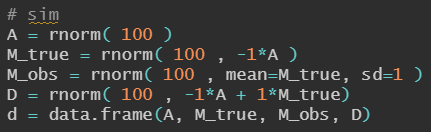
\includegraphics[scale=0.8]{descendant5_code.png}
				\caption*{(c) R code}
			\end{figure}
			%
			\textcolor{blue}{Implications},
			%
			\begin{itemize}
				\item \ndsep{Mt}{D} \\
				\item \ndsep{Mt}{D} \; | A {\small (not possible)}
				\item \ndsep{Mo}{D} \; | A {\small (partially)}
			\end{itemize}
			%
		\end{column}
		%
		\begin{column}{0.5\textwidth}  
			%
			\begin{equ}
				%
				M = \left\{ \begin{aligned} 
					A \leftarrow & \; f_{A}(U_{A}) \\
					Mt \leftarrow & \; f_{M}(A,U_{M}) \\
					Mo \leftarrow & \; f_{M}(Mt, U_{O}) \\
					D \leftarrow & \; f_{D}(A, Mt, U_{D}) \\
					U \sim & \; P(\pmb{U})
					%
				\end{aligned} \right
				%
				\caption*{(a) structural model}
				%
			\end{equ}
			%
			\begin{figure}
				%
				\begin{tikzpicture}
					% nodes
					\node[formula] at (-2.6,0.7) {$U_{O}$};
					\node[formula] at (-2,-0.3) {$Mo$};
					\node[formula] at (-1.7,0.7) {$U_{M}$};
					\node[formula] at (-1,-0.3) {$Mt$};
					\node[formula] at (1,1.5) {$U_{A}$};
					\node[formula] at (0,1) {$A$};
					\node[formula] at (2,0) {$U_{D}$};
					\node[formula] at (1,-0.3) {$D$};
					
					% paths
					\draw [{Circle [open]}-{latex}](-1.6,0.45)--(-1.05,0.05); % Um->Mt
					\draw [-{latex}](-0.9,0)--(0.9,0); % Mt->D
					\draw [{Circle[open]}-{latex}{Circle}](-0.9,0)--(-2,0); % Mt->Mo
					\draw [{Circle [open]}-{latex}](-2.5,0.45)--(-2,0.05); % Uo->Mo
					\draw [{Circle [open]}-{latex}{Circle}](1.7,0)--(0.9,0); % Ud->D
					\draw [{Circle [color=red]}-{latex}](0.1,0.8)--(-0.9,0.1); % A->M
					\draw [-{latex}](0.1,0.75)--(0.9,0.1); % A->D
					\draw [{Circle [open]}-{latex}](0.9,1.3)--(0.1,0.8); % Ua->A
				\end{tikzpicture}
				%
				\caption*{(b) causal diagram}
				%
			\end{figure}
			%
		\end{column}
		%
	\end{columns}
	%
\end{frame}
%
%
\begin{frame}
	{So, what does the simulation means?}
	
	\begin{figure*}
		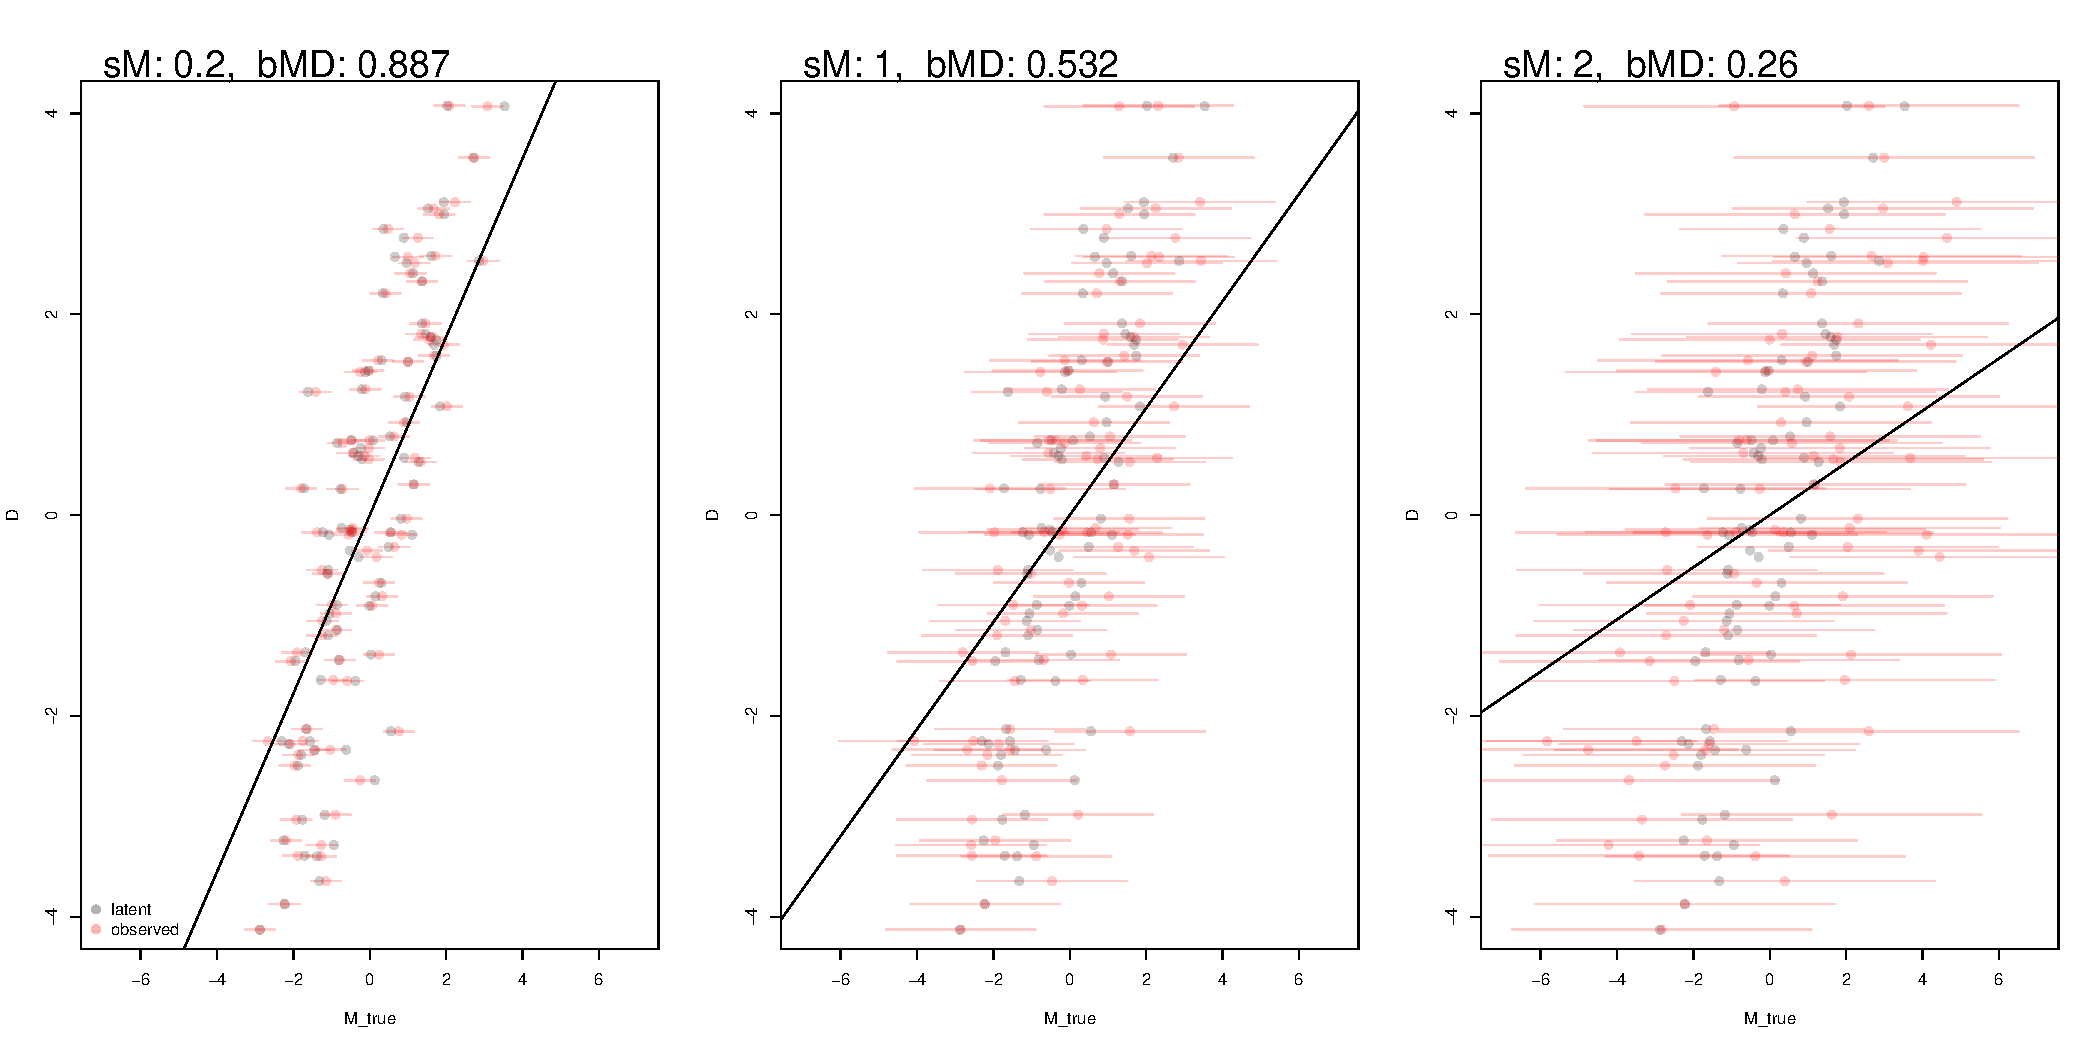
\includegraphics[width=\linewidth]{descendant5_me1.pdf}
	\end{figure*}
	%
\end{frame}
%
%
\begin{frame}
	{So, what does the simulation means?}
	
	\begin{figure*}
		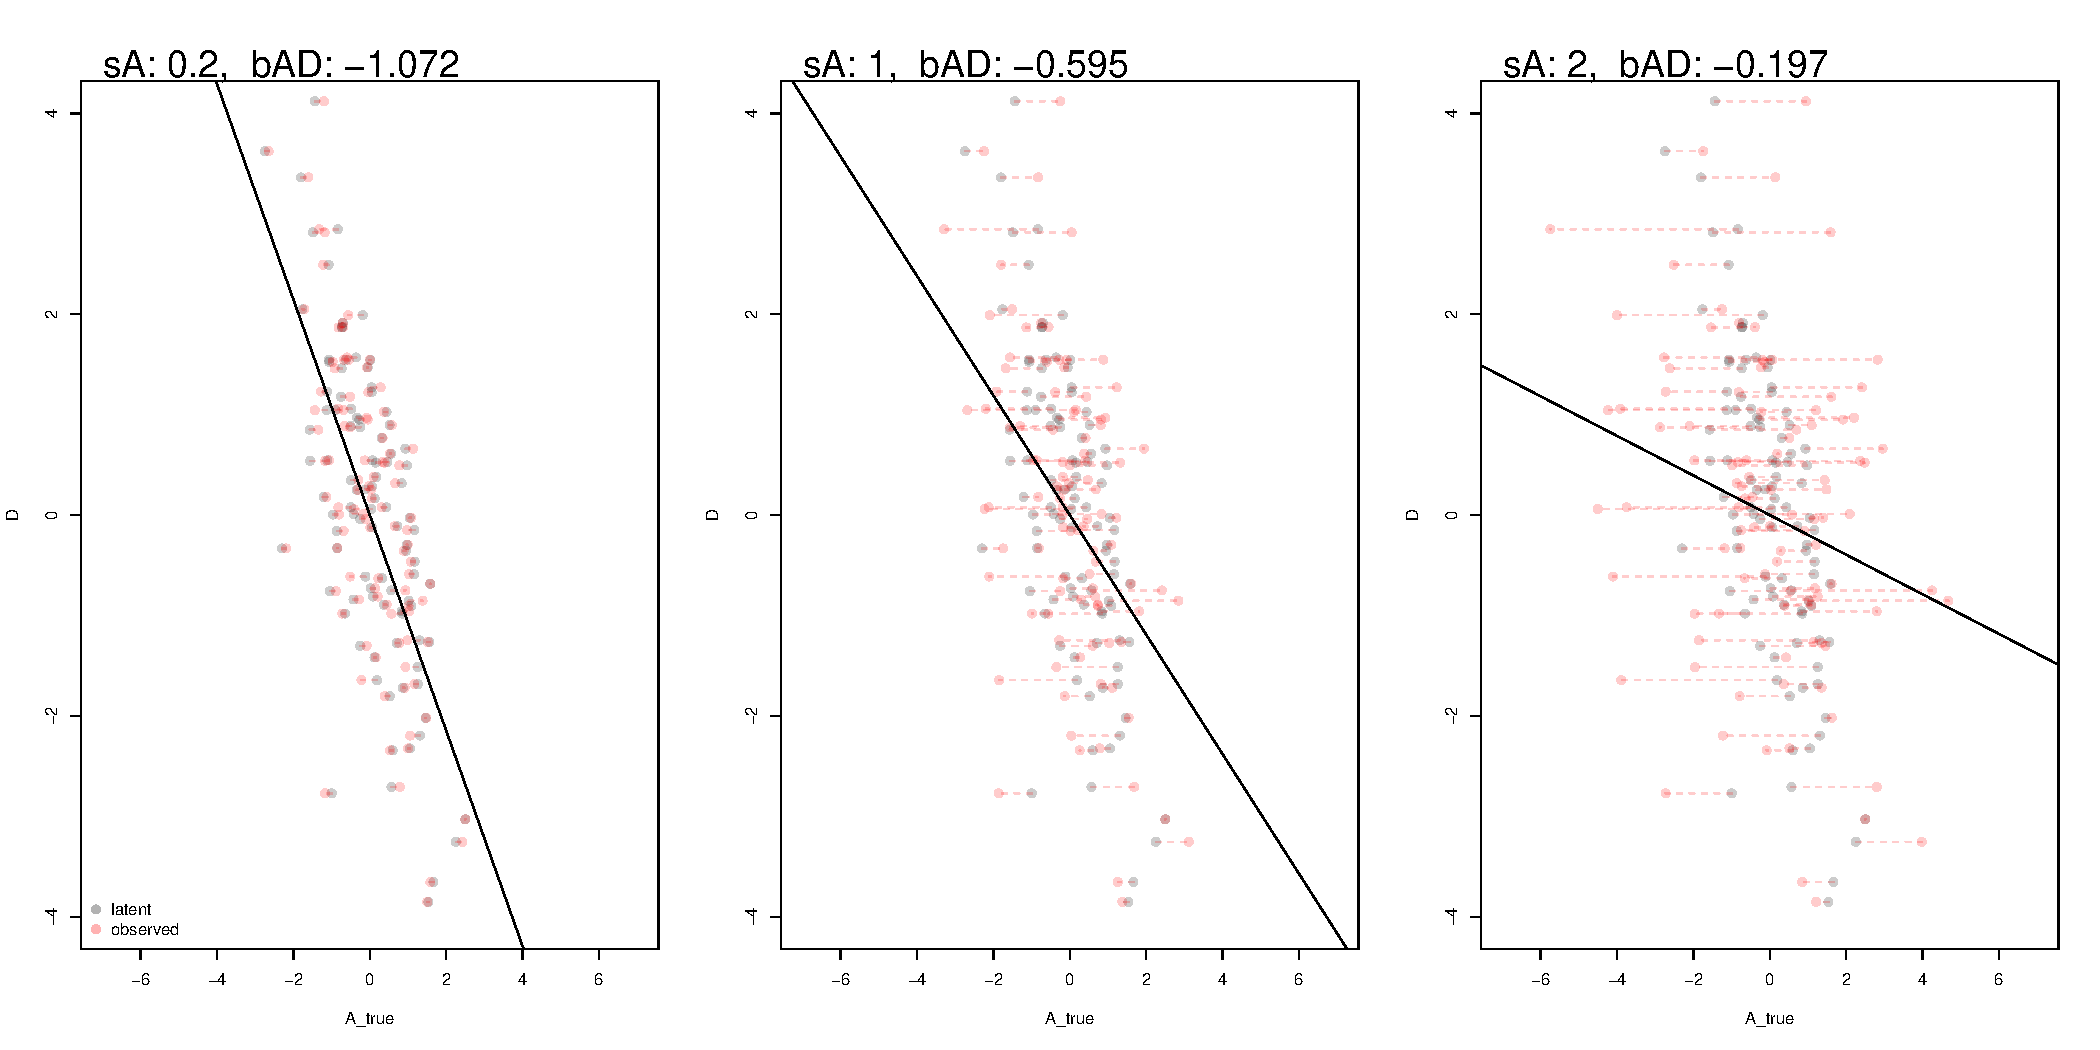
\includegraphics[width=\linewidth]{descendant5_me2.pdf}
	\end{figure*}
	%
\end{frame}
%
%
\begin{lhframe}[rhgraphic={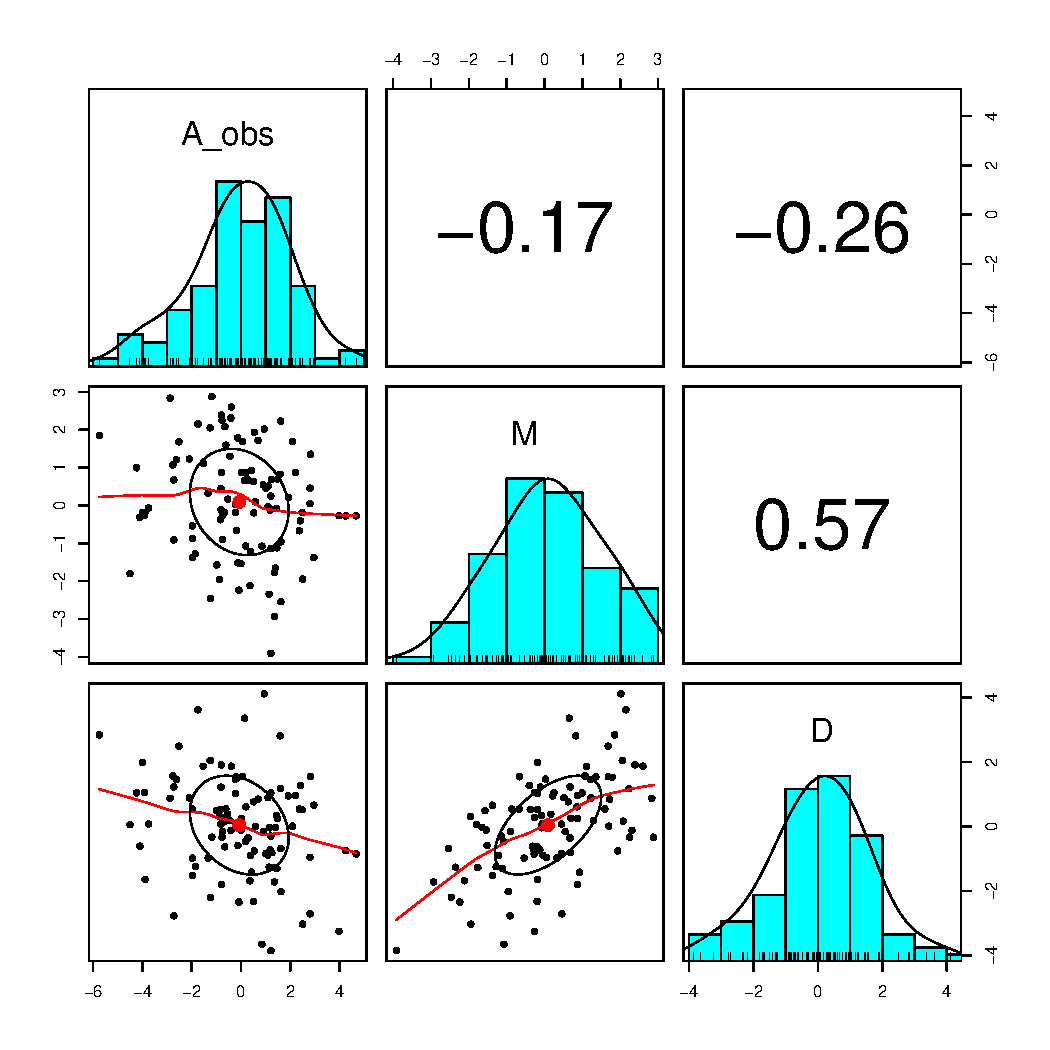
\includegraphics[scale=0.4]{descendant5_panel.pdf}}]
	{``Eyeballing" analysis}
	
	based on \textcolor{blue}{correlation analysis},
	%
	\begin{itemize}
		%
		\item $cor(A, D)<0$ and $cor(M_{obs}, D)>0$
		goes in line of our ``rudimentary" understanding of the data.
		%
		\item we \textcolor{blue}{include} $M$ as a covariate in our statistical model \\
		{\small (besides, it is our research hypothesis)}
		%
	\end{itemize}
	%
\end{lhframe}
%
%
\begin{lhframe}[rhgraphic={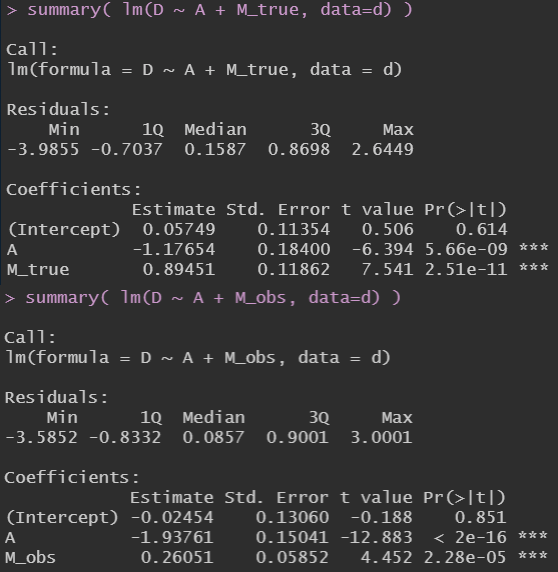
\includegraphics[scale=0.3]{descendant5_reg.png}}]
	{Regression, regression!!}
	
	based on \textcolor{blue}{statistical analysis},
	%
	\begin{itemize}
		%
		\item first model is impossible (\textcolor{blue}{unobservable})
		\item \textcolor{blue}{huge} effect bias in \textcolor{blue}{observable} data (M  and A) \\
		{\small (effect of measurement error, A has less error in its measures)}
		\item we have \textcolor{blue}{smaller} standard error \\
		{\small (not only changes the hypothesis, but also makes you believe you have more precision)}
		%
	\end{itemize}
	%
\end{lhframe}
%
%
\begin{lhframe}[rhgraphic={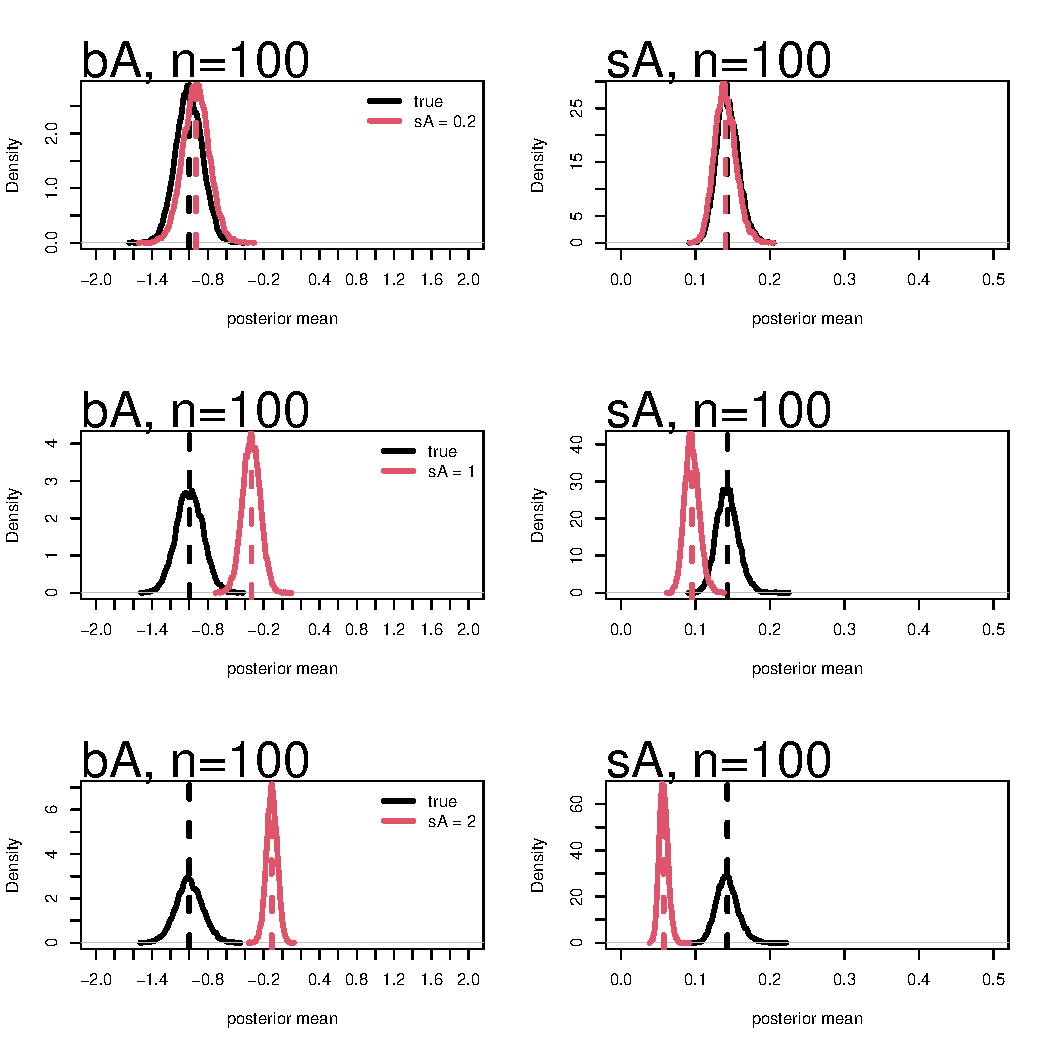
\includegraphics[scale=0.45]{descendant5_samplesize.pdf}}]
	{So, what is going on?}
	
	imagine we can continue sampling,
	%
	\begin{itemize}
		%
		\item $10,000$ samples $n=100$
		%
	\end{itemize}
	
	notice,
	%
	\begin{itemize}
		%
		\item the larger the \textcolor{blue}{measurement error}, the \textcolor{blue}{more confident} you are of your estimates,
		%
		\item larger \textcolor{blue}{measurement error} (in predictor) \textcolor{blue}{hugely bias} the effects, \\
		{\small (also for A, not shown)}
		%
	\end{itemize}
	%
\end{lhframe}
%
%
\begin{frame}
	{How can I fix it???}
	%
	\begin{columns}
		%
		\begin{column}{0.5\textwidth}
			%
			\begin{equ}
				%
				\begin{aligned} 
					D \sim & \; N( \mu, \sigma_{D}) \\
					\mu = & \; \alpha + \beta_{AD} A + \beta_{MD} M_{true} \\
					M_{obs} \sim & \; N( M_{true}, \sigma_{O}) \\
					M_{true} \sim & \; N( 0, \sigma_{M})
				\end{aligned}
				%
				\caption*{(c) probabilistic model}
				%
			\end{equ}
			%
			based on \textcolor{blue}{DAG} and \textcolor{blue}{statistical model}, \\
			use the knowledge of the system
			%
			\begin{itemize}
				%
				\item measurement error part: $M_{obs} \sim N( M_{true}, \sigma_{O})$, 
				%
				\item latent structure: $M_{true} \sim N( 0, \sigma_{M} )$,
				%
				\item latent regression: $\mu = f(A, M_{true})$
				%
			\end{itemize}
			%
		\end{column}
		%
		\begin{column}{0.5\textwidth}  
			%
			\begin{equ}
				%
				M = \left\{ \begin{aligned} 
					A \leftarrow & \; f_{A}(U_{A}) \\
					Mt \leftarrow & \; f_{M}(A,U_{M}) \\
					Mo \leftarrow & \; f_{M}(Mt, U_{O}) \\
					D \leftarrow & \; f_{D}(A, Mt, U_{D}) \\
					U \sim & \; P(\pmb{U})
					%
				\end{aligned} \right
				%
				\caption*{(a) structural model}
				%
			\end{equ}
			%
			\begin{figure}
				%
				\begin{tikzpicture}
					% nodes
					\node[formula] at (-2.6,0.7) {$U_{O}$};
					\node[formula] at (-2,-0.3) {$Mo$};
					\node[formula] at (-1.7,0.7) {$U_{M}$};
					\node[formula] at (-1,-0.3) {$Mt$};
					\node[formula] at (1,1.5) {$U_{A}$};
					\node[formula] at (0,1) {$A$};
					\node[formula] at (2,0) {$U_{D}$};
					\node[formula] at (1,-0.3) {$D$};
					
					% paths
					\draw [{Circle [open]}-{latex}](-1.6,0.45)--(-1.05,0.05); % Um->Mt
					\draw [-{latex}](-0.9,0)--(0.9,0); % Mt->D
					\draw [{Circle[open]}-{latex}{Circle}](-0.9,0)--(-2,0); % Mt->Mo
					\draw [{Circle [open]}-{latex}](-2.5,0.45)--(-2,0.05); % Uo->Mo
					\draw [{Circle [open]}-{latex}{Circle}](1.7,0)--(0.9,0); % Ud->D
					\draw [{Circle [color=red]}-{latex}](0.1,0.8)--(-0.9,0.1); % A->M
					\draw [-{latex}](0.1,0.75)--(0.9,0.1); % A->D
					\draw [{Circle [open]}-{latex}](0.9,1.3)--(0.1,0.8); % Ua->A
					
					% extra
					\node at (0,-0.25) {$(?)$}; % symbol
				\end{tikzpicture}
				%
				\caption*{(b) causal diagram}
				%
			\end{figure}
			%
		\end{column}
		%
	\end{columns}
	%
\end{frame}
%
%
\begin{lhframe}[rhgraphic={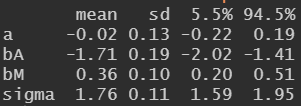
\includegraphics[scale=0.8]{descendant5_reg3.png}}]
	{How can I fix it???}
	
	\begin{figure}
		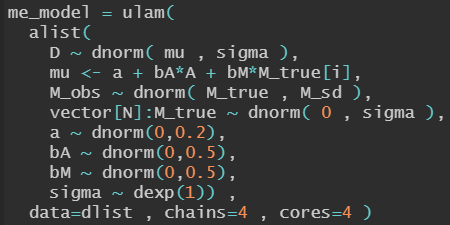
\includegraphics[scale=0.7]{descendant5_code2.png}
	\end{figure}
	%
	
	Using \textcolor{blue}{DAG} and \textcolor{blue}{Bayesian} analysis: \\
	{\small \textcolor{blue}{(frequentist analysis falls short here)}}
	%
	\begin{itemize}
		%
		\item measurement error part: $M_{obs} \sim N( M_{true}, \sigma_{O})$, 
		%
		\item latent structure: $M_{true} \sim N( 0, \sigma_{M} )$,
		%
		\item latent regression: $\mu = f(A, M_{true})$
		%
	\end{itemize}
	%
\end{lhframe}
%
%
%%%%%%%%%%%%%%%%%%%%%%%%%%%%%%%%%%%%%%%%%%%%%%%%%%%%%%%%%%%
\subsection{Descendant: measurement error, both}
%%%%%%%%%%%%%%%%%%%%%%%%%%%%%%%%%%%%%%%%%%%%%%%%%%%%%%%%%%%
%
%
\begin{frame}[t, negative]
	\subsectionpage
\end{frame}
%
%
\begin{frame}
	{Measurement error, both}
	%
	\begin{columns}
		%
		\begin{column}{0.5\textwidth}
			%			
			variables\footnote{\citet{McElreath_2020}, chapter 15 (p. 495)},
			%
			\begin{itemize}
				%
				\item A, median age at marriage
				\item Mt, (\textit{true}) marriage rate 
				\item Mo, (\textit{observed}) marriage rate
				\item Dt, (\textit{true}) divorce rate 
				\item Do, (\textit{observed}) divorce rate
				%
			\end{itemize}
			%
			
			extras,
			%
			\begin{itemize}
				%
				\item $U_{M}$, between variability (\textit{true} rate)
				\item $U_{D}$, between variability (\textit{true} rate)
				\item $U_{O1}$, measurement error
				\item $U_{O2}$, measurement error
				%
			\end{itemize}
			%
		\end{column}
		%
		\begin{column}{0.5\textwidth}  
			%
			\begin{equ}
				%
				M = \left\{ \begin{aligned} 
					A \leftarrow & \; f_{A}(U_{A}) \\
					Mt \leftarrow & \; f_{M}(A,U_{M}) \\
					Mo \leftarrow & \; f_{M}(Mt, U_{O1}) \\
					Dt \leftarrow & \; f_{D}(A, M, U_{D}) \\
					Do \leftarrow & \; f_{D}(Dt, U_{O2}) \\
					U \sim & \; P(\pmb{U})
					%
				\end{aligned} \right
				%
				\caption*{(a) structural model}
				%
			\end{equ}
			%
			\begin{figure}
				%
				\begin{tikzpicture}
					% nodes
					\node[formula] at (-2.6,0.7) {$U_{O1}$};
					\node[formula] at (-2,-0.3) {$Mo$};
					\node[formula] at (-1.7,0.7) {$U_{M}$};
					\node[formula] at (-1,-0.3) {$Mt$};
					\node[formula] at (1,1.5) {$U_{A}$};
					\node[formula] at (0,1) {$A$};
					\node[formula] at (1.8,0.7) {$U_{D}$};
					\node[formula] at (1,-0.3) {$Dt$};
					\node[formula] at (2.7,0.7) {$U_{O2}$};
					\node[formula] at (1.95,-0.3) {$Do$};
					
					% paths
					\draw [{Circle [open]}-{latex}](-1.6,0.45)--(-1.05,0.05); % Um->Mt
					\draw [-{latex}](-0.9,0)--(0.9,0); % Mt->Dt
					\draw [{Circle [open]}-{latex}{Circle}](0.9,0)--(2,0); % Dt->Do
					\draw [{Circle [open]}-{latex}](1.7,0.5)--(1.05,0.05); % Ud->Dt
					\draw [{Circle [open]}-{latex}](2.6,0.5)--(2,0.05); % Uo->Do
					\draw [{Circle[open]}-{latex}{Circle}](-0.9,0)--(-2,0); % Mt->Mo
					\draw [{Circle [open]}-{latex}](-2.5,0.45)--(-2,0.05); % Uo->Mo
					\draw [{Circle [color=red]}-{latex}](0.1,0.8)--(-0.9,0.1); % A->M
					\draw [-{latex}](0.1,0.75)--(0.9,0.1); % A->D
					\draw [{Circle [open]}-{latex}](0.9,1.3)--(0.1,0.8); % Ua->A
					
					% extra
					\node at (0,-0.25) {$(?)$}; % symbol
				\end{tikzpicture}
				%
				\caption*{(b) causal diagram}
				%
			\end{figure}
			%
		\end{column}
		%
	\end{columns}
	%
\end{frame}
%
%
\begin{frame}
	{Simulation setting}
	%
	\begin{columns}
		%
		\begin{column}{0.5\textwidth}
			%
			\begin{figure}
				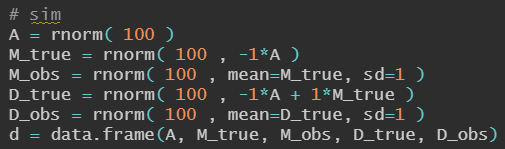
\includegraphics[scale=0.7]{descendant6_code.png}
				\caption*{(c) R code}
			\end{figure}
			%
			\textcolor{blue}{Implications},
			%
			\begin{itemize}
				\item \ndsep{Mt}{Dt} \\
				\item \ndsep{Mt}{Dt} \; | A {\small (not possible)} 
				\item \ndsep{Mo}{Do} \\
				\item \ndsep{Mo}{Do} \; | A 
			\end{itemize}
			%
		\end{column}
		%
		\begin{column}{0.5\textwidth}  
			%
			\begin{equ}
				%
				M = \left\{ \begin{aligned} 
					A \leftarrow & \; f_{A}(U_{A}) \\
					Mt \leftarrow & \; f_{M}(A,U_{M}) \\
					Mo \leftarrow & \; f_{M}(Mt, U_{O1}) \\
					Dt \leftarrow & \; f_{D}(A, M, U_{D}) \\
					Do \leftarrow & \; f_{D}(Dt, U_{O2}) \\
					U \sim & \; P(\pmb{U})
					%
				\end{aligned} \right
				%
				\caption*{(a) structural model}
				%
			\end{equ}
			%
			\begin{figure}
				%
				\begin{tikzpicture}
					% nodes
					\node[formula] at (-2.6,0.7) {$U_{O1}$};
					\node[formula] at (-2,-0.3) {$Mo$};
					\node[formula] at (-1.7,0.7) {$U_{M}$};
					\node[formula] at (-1,-0.3) {$Mt$};
					\node[formula] at (1,1.5) {$U_{A}$};
					\node[formula] at (0,1) {$A$};
					\node[formula] at (1.8,0.7) {$U_{D}$};
					\node[formula] at (1,-0.3) {$Dt$};
					\node[formula] at (2.7,0.7) {$U_{O2}$};
					\node[formula] at (1.95,-0.3) {$Do$};
					
					% paths
					\draw [{Circle [open]}-{latex}](-1.6,0.45)--(-1.05,0.05); % Um->Mt
					\draw [-{latex}](-0.9,0)--(0.9,0); % Mt->Dt
					\draw [{Circle [open]}-{latex}{Circle}](0.9,0)--(2,0); % Dt->Do
					\draw [{Circle [open]}-{latex}](1.7,0.5)--(1.05,0.05); % Ud->Dt
					\draw [{Circle [open]}-{latex}](2.6,0.5)--(2,0.05); % Uo->Do
					\draw [{Circle[open]}-{latex}{Circle}](-0.9,0)--(-2,0); % Mt->Mo
					\draw [{Circle [open]}-{latex}](-2.5,0.45)--(-2,0.05); % Uo->Mo
					\draw [{Circle [color=red]}-{latex}](0.1,0.8)--(-0.9,0.1); % A->M
					\draw [-{latex}](0.1,0.75)--(0.9,0.1); % A->D
					\draw [{Circle [open]}-{latex}](0.9,1.3)--(0.1,0.8); % Ua->A
				\end{tikzpicture}
				%
				\caption*{(b) causal diagram}
				%
			\end{figure}
			%
		\end{column}
		%
	\end{columns}
	%
\end{frame}
%
%
\begin{lhframe}[rhgraphic={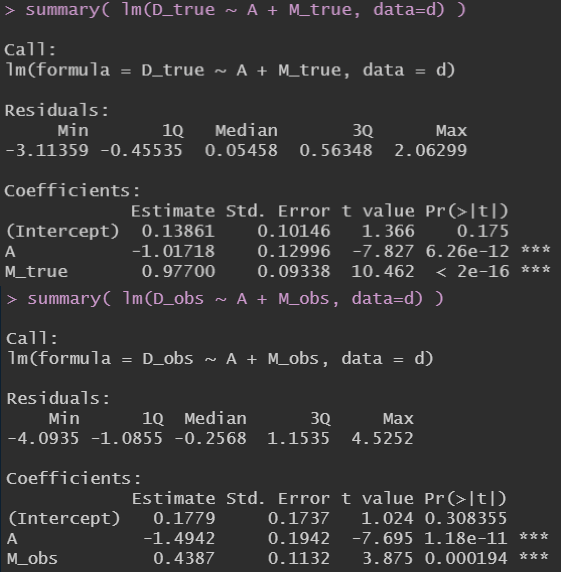
\includegraphics[scale=0.3]{descendant6_reg.png}}]
	{Regression, regression!!}
	
	based on \textcolor{blue}{statistical analysis},
	%
	\begin{itemize}
		%
		\item first model is impossible (\textcolor{blue}{unobservable})
		\item \textcolor{blue}{huge} effect bias in \textcolor{blue}{observable} data (M  and A) \\
		{\small (effect of measurement error, A has less error in its measures)}
		\item we have \textcolor{blue}{smaller} standard error \\
		{\small (not only changes the hypothesis, but also makes you believe you have more precision)}
		%
	\end{itemize}
	%
\end{lhframe}
%
%
\begin{lhframe}[rhgraphic={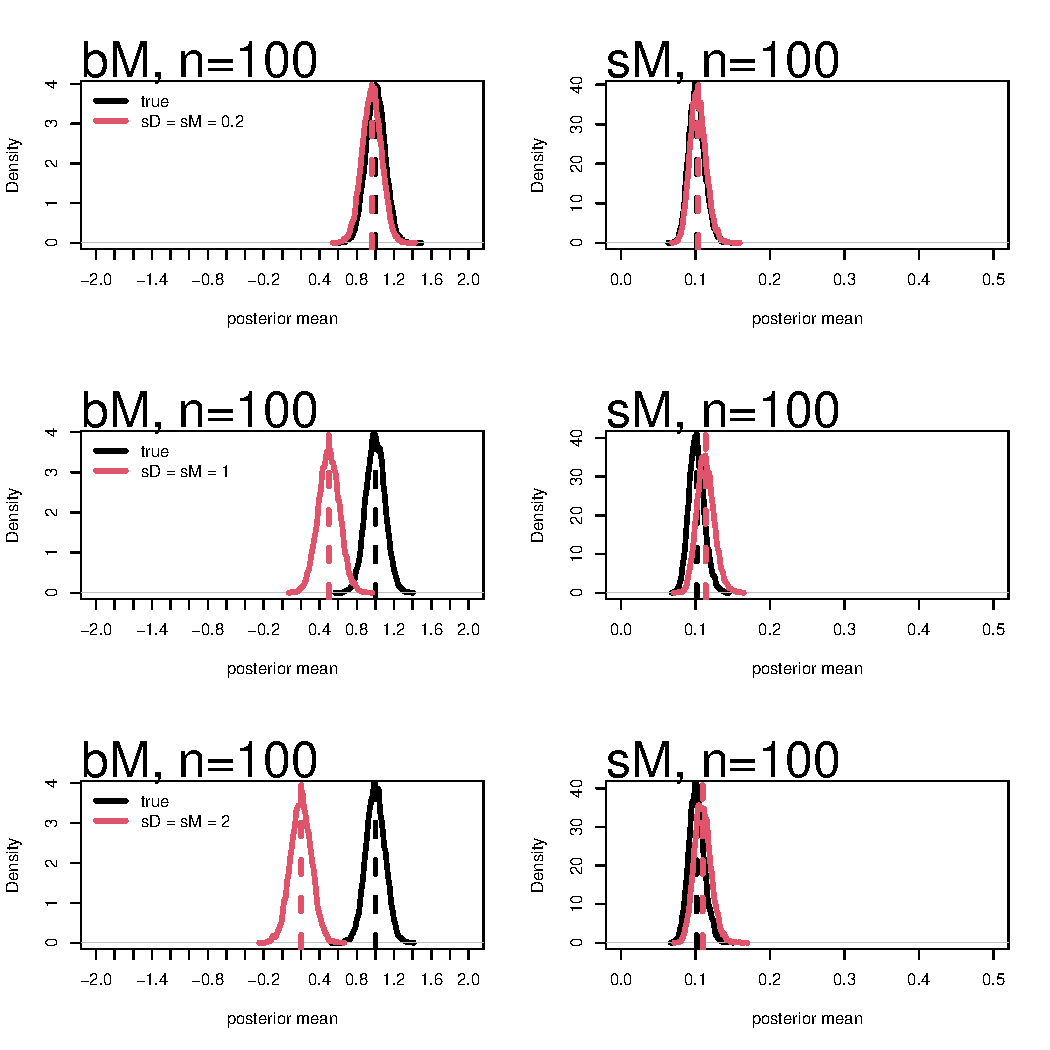
\includegraphics[scale=0.45]{descendant6_samplesize.pdf}}]
	{So, what is going on?}
	
	imagine we can continue sampling,
	%
	\begin{itemize}
		%
		\item $10,000$ samples $n=100$
		%
	\end{itemize}
	
	notice,
	%
	\begin{itemize}
		%
		\item now it is unclear the direction our \textcolor{blue}{precision (standard error)} would go with larger \textcolor{blue}{measurement error},
		%
		\item however, the larger \textcolor{blue}{measurement error} (in predictor) \textcolor{blue}{hugely bias} the effects, \\
		{\small (also for A, not shown)}
		%
	\end{itemize}
	%
\end{lhframe}
%
%
\begin{frame}
	{How can I fix it???}
	%
	\begin{columns}
		%
		\begin{column}{0.5\textwidth}
			%
			\begin{equ}
				%
				\begin{aligned} 
					D_{obs} \sim & \; N( D_{true}, \sigma_{O1}) \\
					D_{true} \sim & \; N( \mu, \sigma_{D}) \\
					\mu = & \; \alpha + \beta_{AD} A + \beta_{MD} M_{true} \\
					M_{obs} \sim & \; N( M_{true}, \sigma_{O2}) \\
					M_{true} \sim & \; N( 0, \sigma_{M})
				\end{aligned}
				%
				\caption*{(c) probabilistic model}
				%
			\end{equ}
			%
			based on \textcolor{blue}{DAG} and \textcolor{blue}{statistical model}, \\
			(use the knowledge of the system).
			
		\end{column}
		%
		\begin{column}{0.5\textwidth}  
			%
			\begin{equ}
				%
				M = \left\{ \begin{aligned} 
					A \leftarrow & \; f_{A}(U_{A}) \\
					Mt \leftarrow & \; f_{M}(A,U_{M}) \\
					Mo \leftarrow & \; f_{M}(Mt, U_{O1}) \\
					Dt \leftarrow & \; f_{D}(A, M, U_{D}) \\
					Do \leftarrow & \; f_{D}(Dt, U_{O2}) \\
					U \sim & \; P(\pmb{U})
					%
				\end{aligned} \right
				%
				\caption*{(a) structural model}
				%
			\end{equ}
			%
			\begin{figure}
				%
				\begin{tikzpicture}
					% nodes
					\node[formula] at (-2.6,0.7) {$U_{O1}$};
					\node[formula] at (-2,-0.3) {$Mo$};
					\node[formula] at (-1.7,0.7) {$U_{M}$};
					\node[formula] at (-1,-0.3) {$Mt$};
					\node[formula] at (1,1.5) {$U_{A}$};
					\node[formula] at (0,1) {$A$};
					\node[formula] at (1.8,0.7) {$U_{D}$};
					\node[formula] at (1,-0.3) {$Dt$};
					\node[formula] at (2.7,0.7) {$U_{O2}$};
					\node[formula] at (1.95,-0.3) {$Do$};
					
					% paths
					\draw [{Circle [open]}-{latex}](-1.6,0.45)--(-1.05,0.05); % Um->Mt
					\draw [-{latex}](-0.9,0)--(0.9,0); % Mt->Dt
					\draw [{Circle [open]}-{latex}{Circle}](0.9,0)--(2,0); % Dt->Do
					\draw [{Circle [open]}-{latex}](1.7,0.5)--(1.05,0.05); % Ud->Dt
					\draw [{Circle [open]}-{latex}](2.6,0.5)--(2,0.05); % Uo->Do
					\draw [{Circle[open]}-{latex}{Circle}](-0.9,0)--(-2,0); % Mt->Mo
					\draw [{Circle [open]}-{latex}](-2.5,0.45)--(-2,0.05); % Uo->Mo
					\draw [{Circle [color=red]}-{latex}](0.1,0.8)--(-0.9,0.1); % A->M
					\draw [-{latex}](0.1,0.75)--(0.9,0.1); % A->D
					\draw [{Circle [open]}-{latex}](0.9,1.3)--(0.1,0.8); % Ua->A
					
					% extra
					\node at (0,-0.25) {$(?)$}; % symbol
				\end{tikzpicture}
				%
				\caption*{(b) causal diagram}
				%
			\end{figure}
			%
		\end{column}
		%
	\end{columns}
	%
\end{frame}
%
%
\begin{lhframe}[rhgraphic={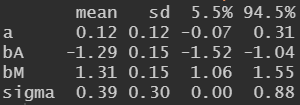
\includegraphics[scale=0.8]{descendant6_reg3.png}}]
	{How can I fix it???}
	
	\begin{figure}
		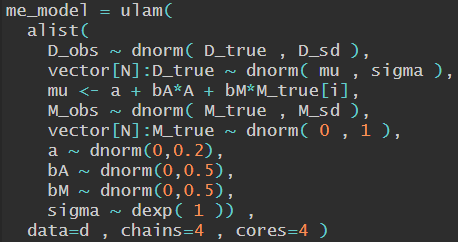
\includegraphics[scale=0.7]{descendant6_code2.png}
	\end{figure}
	%
	
	Using \textcolor{blue}{DAG} and \textcolor{blue}{Bayesian} analysis: \\
	{\small \textcolor{blue}{(frequentist analysis falls short here)}}
	%
\end{lhframe}
%
%
%%%%%%%%%%%%%%%%%%%%%%%%%%%%%%%%%%%%%%%%%%%%%%%%%%%%%%%%%%%
\subsection{Descendant: censoring, outcome only}
%%%%%%%%%%%%%%%%%%%%%%%%%%%%%%%%%%%%%%%%%%%%%%%%%%%%%%%%%%%
%
%
\begin{frame}[t, negative]
	\subsectionpage
\end{frame}
%
%	
\begin{frame}
	{Censoring, outcome only\footnote{\citet{Ostling_2022}, \citet{Vincent_2022} }}
	%
	\begin{columns}
		%
		\begin{column}{0.5\textwidth}
			%
			also, 
			%
			\begin{itemize}
				%
				\item think of \textcolor{blue}{hurdle} or \textcolor{blue}{zero-inflated} models
				%
			\end{itemize}
			
			research question, 
			%
			\begin{itemize}
				%
				\item \textcolor{blue}{Does $E$ has a (direct) effect on $I$?}
				%
			\end{itemize}
			
			variables,
			%
			\begin{itemize}
				%
				\item SES, socio economical status
				\item E, education
				\item If, income (\textit{fully observed})
				\item Ic, income (\textit{right censored})
				%
			\end{itemize}
			%
			
			extras,
			%
			\begin{itemize}
				%
				\item $U_{I}$, between variability
				\item $U_{C}$, censoring mechanism
				%
			\end{itemize}
			%
		\end{column}
		%
		\begin{column}{0.5\textwidth}  
			%
			\begin{equ}
				%
				M = \left\{ \begin{aligned} 
					SES \leftarrow & \; f_{S}(U_{S}) \\
					E \leftarrow & \; f_{E}(SES,U_{E}) \\
					If \leftarrow & \; f_{I}(E, SES, U_{I}) \\
					Ic \leftarrow & \; f_{I}(Ic, U_{C}) \\
					U \sim & \; P(\pmb{U})
					%
				\end{aligned} \right
				%
				\caption*{(a) structural model}
				%
			\end{equ}
			%
			\begin{figure}
				%
				\begin{tikzpicture}
					% nodes
					\node[formula] at (-2,0) {$U_{E}$};
					\node[formula] at (-1,-0.3) {$E$};
					\node[formula] at (1,1.5) {$U_{S}$};
					\node[formula] at (-0.3,1) {$SES$};
					\node[formula] at (1.8,0.7) {$U_{I}$};
					\node[formula] at (1,-0.3) {$If$};
					\node[formula] at (2.7,0.7) {$U_{C}$};
					\node[formula] at (1.95,-0.3) {$Ic$};
					
					% paths
					\draw [{Circle [open]}-{latex}{Circle}](-1.7,0)--(-0.9,0); % Ue->E
					\draw [-{latex}](-0.9,0)--(0.9,0); % E->If
					\draw [{Circle [open]}-{latex}{Circle}](0.9,0)--(2,0); % If->It
					\draw [{Circle [open]}-{latex}](1.7,0.5)--(1.05,0.05); % Ui->If
					\draw [{Circle [open]}-{latex}](2.6,0.5)--(2,0.05); % Ut->It
					\draw [{Circle [color=red]}-{latex}](0.1,0.8)--(-0.9,0.1); % SES->E
					\draw [-{latex}](0.1,0.75)--(0.9,0.1); % SES->If
					\draw [{Circle [open]}-{latex}](0.9,1.3)--(0.1,0.8); % US->SES
					
					% extra
					\node at (0,-0.25) {$(?)$}; % symbol
				\end{tikzpicture}
				%
				\caption*{(b) causal diagram}
				%
			\end{figure}
			%
		\end{column}
		%
	\end{columns}
	%
\end{frame}
%
%
\begin{frame}
	{Simulation setting}
	%
	\begin{columns}
		%
		\begin{column}{0.5\textwidth}
			%
			\begin{figure}
				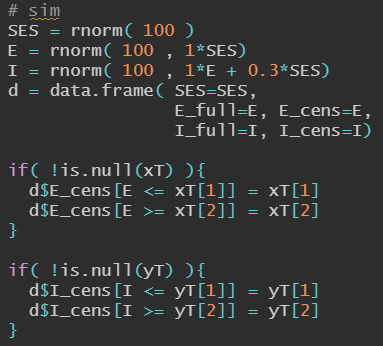
\includegraphics[scale=0.65]{descendant7_code.png}
				\caption*{(c) R code}
			\end{figure}
			%
			\textcolor{blue}{Implications},
			%
			\begin{itemize}
				\item \ndsep{E}{If} \\
				\item \ndsep{E}{If} \; | SES {\small (not possible)}
			\end{itemize}
			%
		\end{column}
		%
		\begin{column}{0.5\textwidth}  
			%
			\begin{equ}
				%
				M = \left\{ \begin{aligned} 
					SES \leftarrow & \; f_{S}(U_{S}) \\
					E \leftarrow & \; f_{E}(SES,U_{E}) \\
					If \leftarrow & \; f_{I}(E, SES, U_{I}) \\
					Ic \leftarrow & \; f_{I}(If, U_{C}) \\
					U \sim & \; P(\pmb{U})
					%
				\end{aligned} \right
				%
				\caption*{(a) structural model}
				%
			\end{equ}
			%
			\begin{figure}
				%
				\begin{tikzpicture}
					% nodes
					\node[formula] at (-2,0) {$U_{E}$};
					\node[formula] at (-1,-0.3) {$E$};
					\node[formula] at (1,1.5) {$U_{S}$};
					\node[formula] at (-0.3,1) {$SES$};
					\node[formula] at (1.8,0.7) {$U_{I}$};
					\node[formula] at (1,-0.3) {$If$};
					\node[formula] at (2.7,0.7) {$U_{C}$};
					\node[formula] at (1.95,-0.3) {$Ic$};
					
					% paths
					\draw [{Circle [open]}-{latex}{Circle}](-1.7,0)--(-0.9,0); % Ue->E
					\draw [-{latex}](-0.9,0)--(0.9,0); % E->If
					\draw [{Circle [open]}-{latex}{Circle}](0.9,0)--(2,0); % If->It
					\draw [{Circle [open]}-{latex}](1.7,0.5)--(1.05,0.05); % Ui->If
					\draw [{Circle [open]}-{latex}](2.6,0.5)--(2,0.05); % Ut->It
					\draw [{Circle [color=red]}-{latex}](0.1,0.8)--(-0.9,0.1); % SES->E
					\draw [-{latex}](0.1,0.75)--(0.9,0.1); % SES->If
					\draw [{Circle [open]}-{latex}](0.9,1.3)--(0.1,0.8); % US->SES
				\end{tikzpicture}
				%
				\caption*{(b) causal diagram}
				%
			\end{figure}
			%
		\end{column}
		%
	\end{columns}
	%
\end{frame}
%
%
\begin{frame}
	{So, what does the simulation means?}
	
	\begin{figure*}
		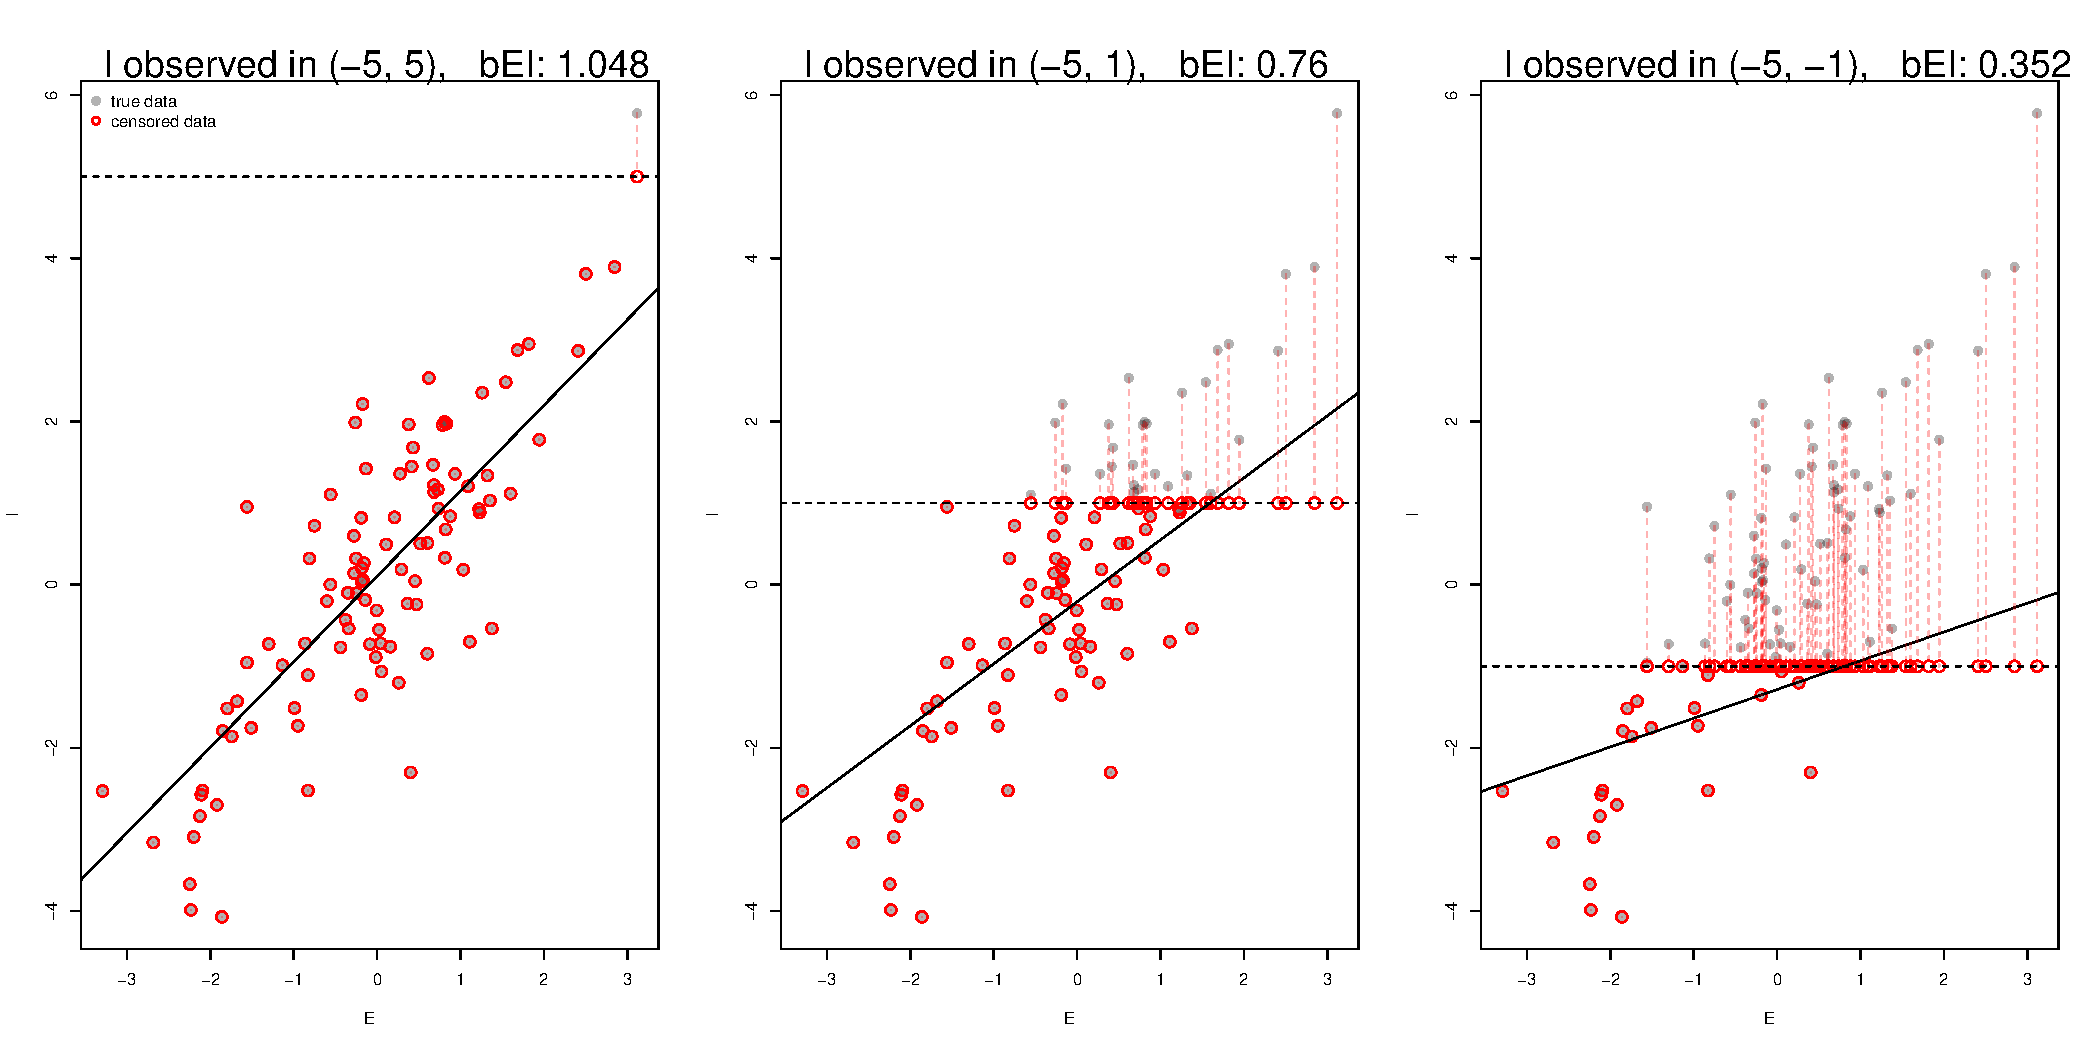
\includegraphics[width=\linewidth]{descendant7_cens1.pdf}
	\end{figure*}
	%
\end{frame}
%
%
\begin{frame}
	{So, what does the simulation means?}
	
	\begin{figure*}
		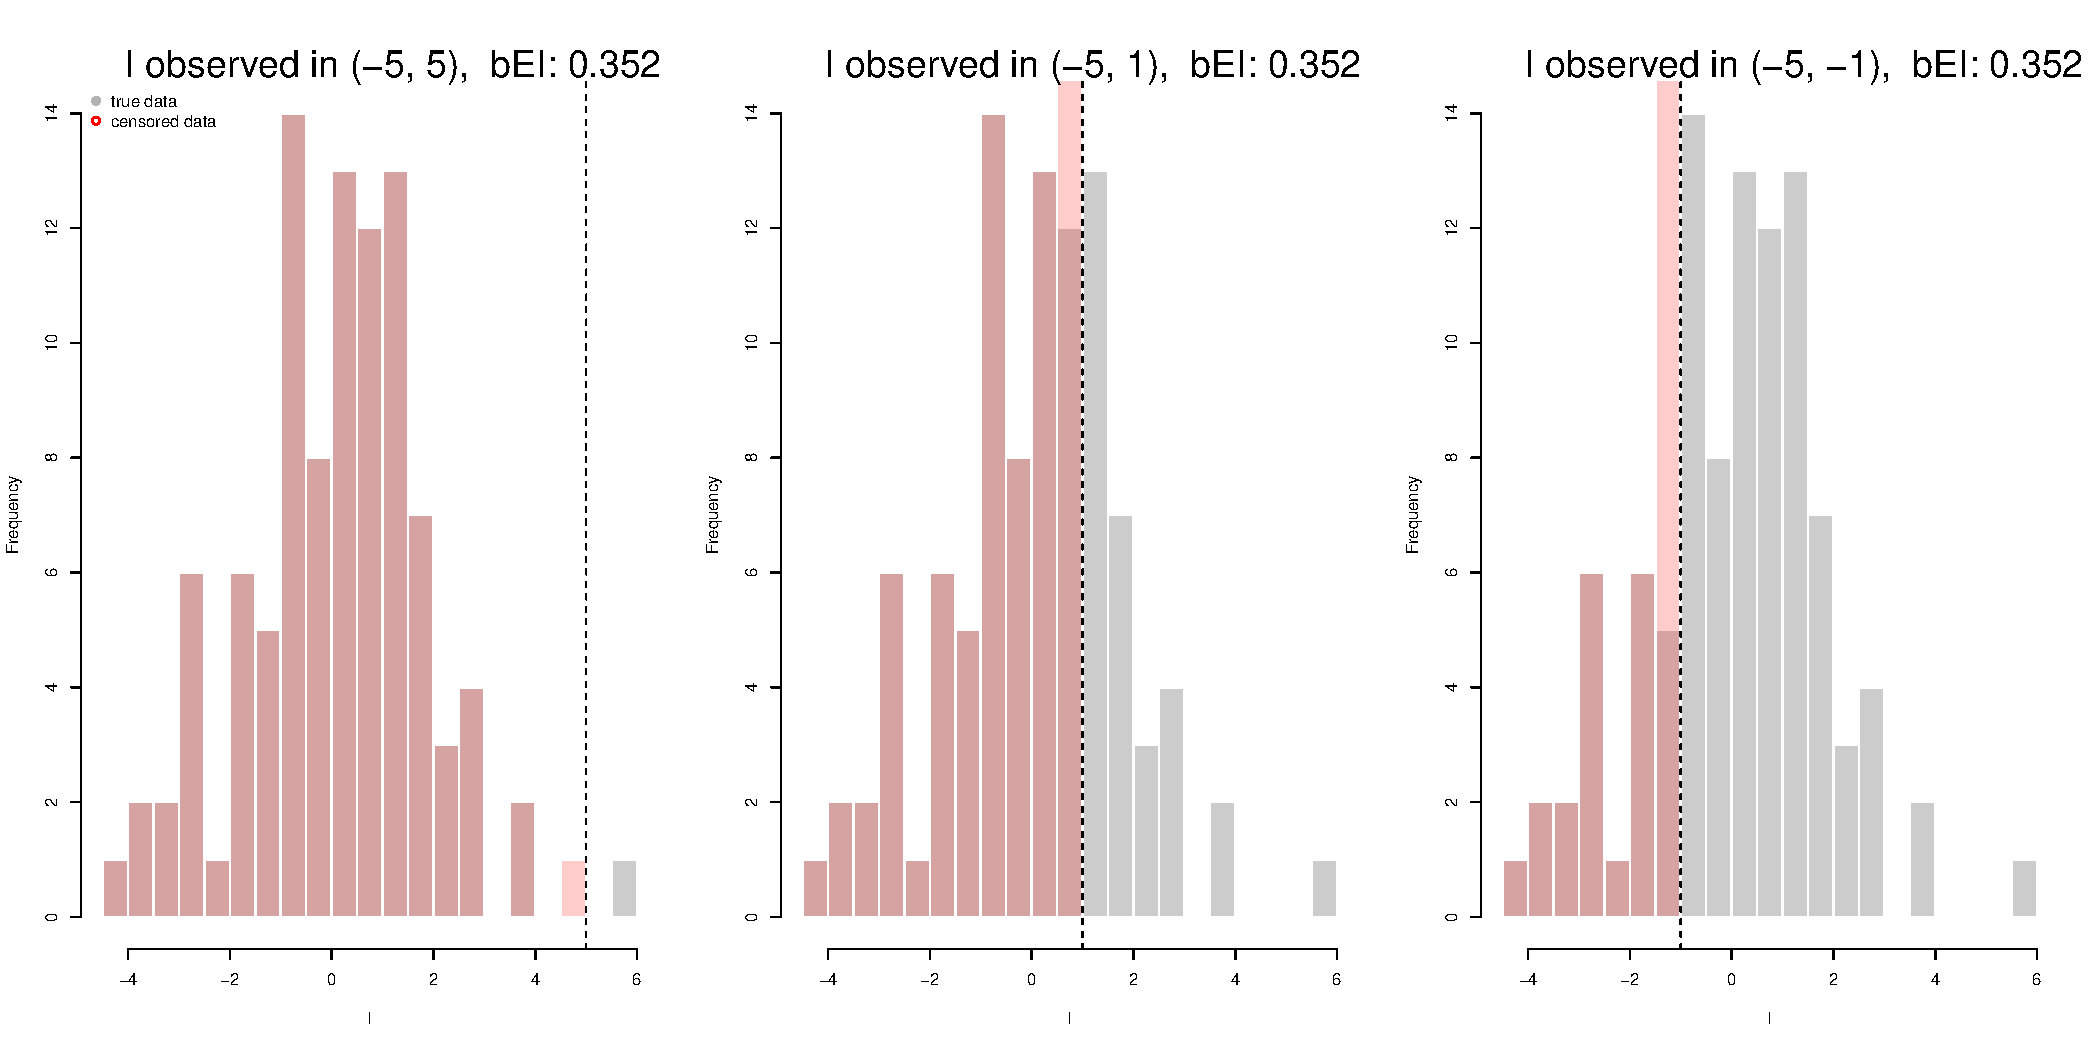
\includegraphics[width=\linewidth]{descendant7_cens2.pdf}
	\end{figure*}
	%
\end{frame}
%
%
\begin{lhframe}[rhgraphic={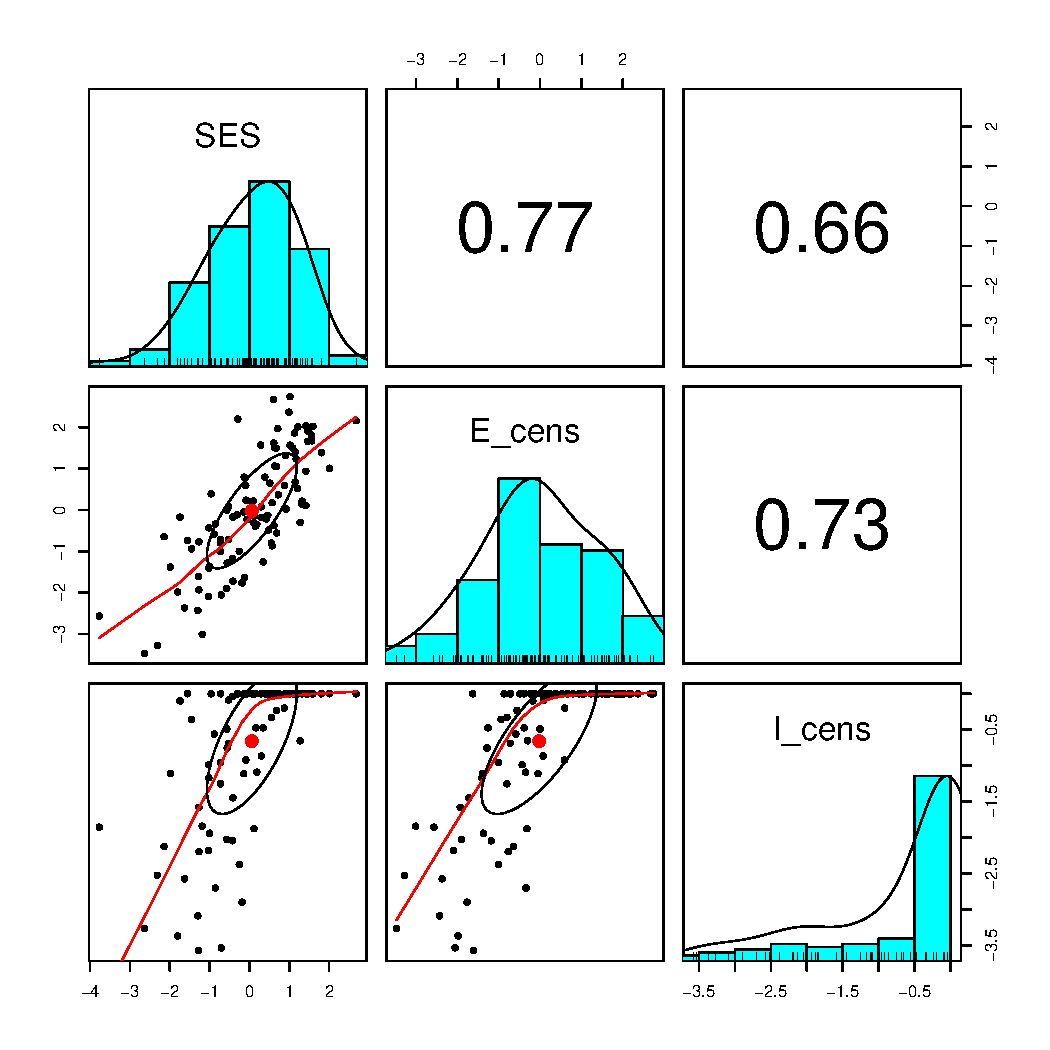
\includegraphics[scale=0.4]{descendant7_panel.pdf}}]
	{``Eyeballing" analysis}
	
	\begin{itemize}
		\item does \textcolor{blue}{correlation analysis} help now?
		\item and how about \textcolor{blue}{step-wise regression?} \\
		\item \textcolor{blue}{highly skewed distribution} of the outcome, so what?
	\end{itemize}
	
\end{lhframe}
%
%
\begin{lhframe}[rhgraphic={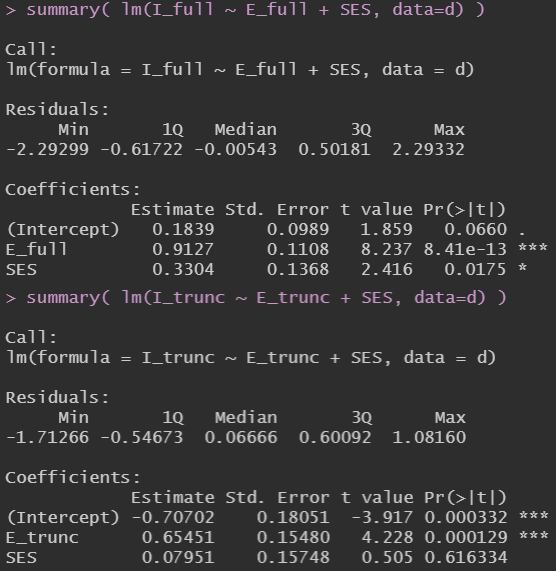
\includegraphics[scale=0.3]{descendant7_reg.png}}]
	{Regression, regression!!}
	
	based on \textcolor{blue}{statistical analysis},
	%
	\begin{itemize}
		%
		\item first model is impossible (\textcolor{blue}{unobservable})
		\item effect \textcolor{blue}{bias} in \textcolor{blue}{censored} data \\
		(E and SES)
		\item we have \textcolor{blue}{smaller} standard errors \\
		{\small (why?? hint: false confidence in measuring one ``range'' of the outcome)}
		%
	\end{itemize}
	%
\end{lhframe}
%
%
\begin{lhframe}[rhgraphic={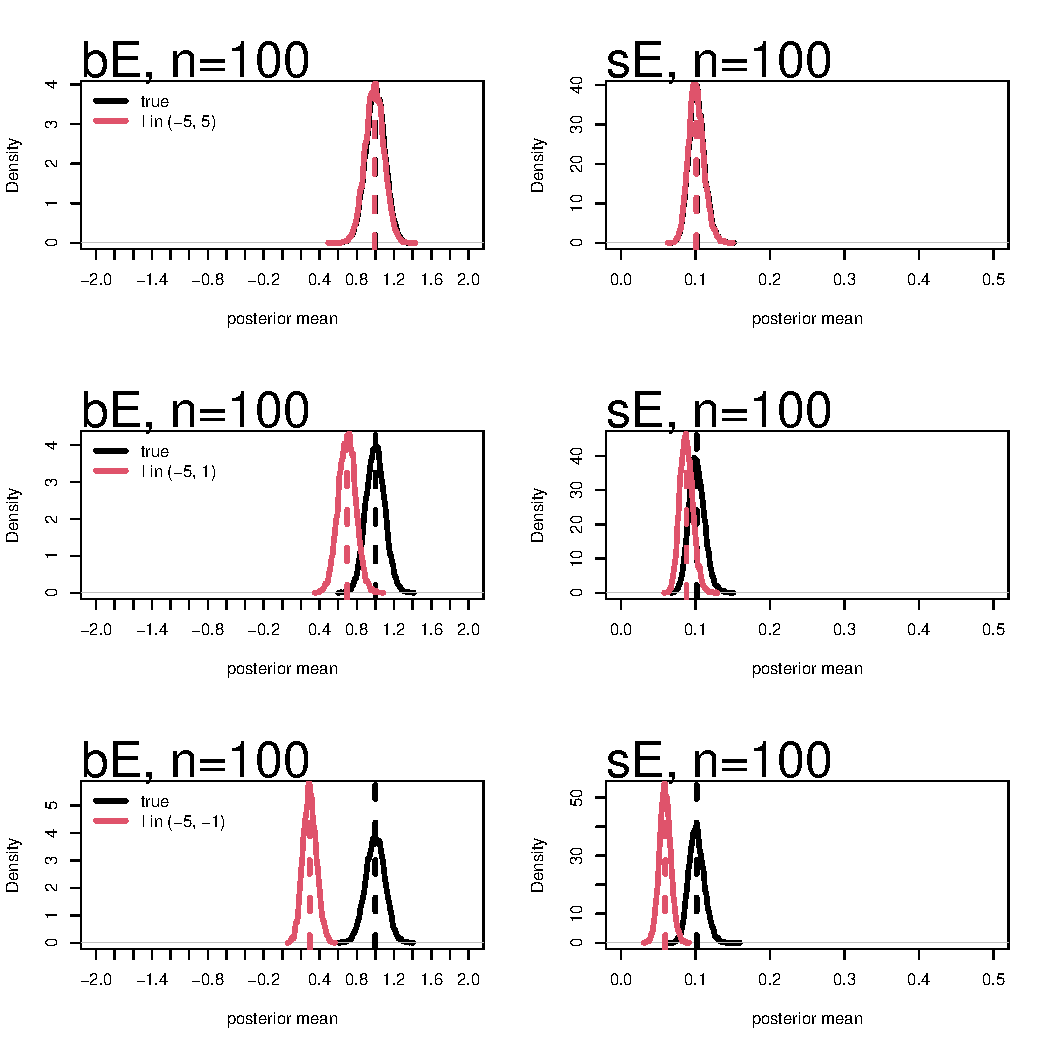
\includegraphics[scale=0.45]{descendant7_samplesize.pdf}}]
	{So, what is going on?}
	
	imagine we can continue sampling,
	%
	\begin{itemize}
		%
		\item $10,000$ samples $n=100$
		%
	\end{itemize}
	
	notice,
	%
	\begin{itemize}
		%
		\item the smaller the \textcolor{blue}{censoring range}, the \textcolor{blue}{more confident} you are of your estimates,
		%
		\item smaller \textcolor{blue}{censoring range} \textcolor{blue}{bias} the effects, \\
		{\small (also for SES, not shown)}
		%
	\end{itemize}
	%
\end{lhframe}
%
%
\begin{frame}
	{How can I fix it???}
	%
	\begin{columns}
		%
		\begin{column}{0.5\textwidth}
			%
			\begin{equ}
				%
				\begin{aligned} 
					I_{nc} \sim & \; N( \mu_{nc} , \sigma_{I} ) \\
					\mu_{nc} = & \; \alpha + \beta_{E} E_{nc} + \beta_{S} SES_{nc} \\
					I_{rc} \sim & \; Nccd( \mu_{rc} , \sigma_{I} ) \\
					\mu_{rc} = & \; \alpha + \beta_{E} E_{rc} + \beta_{S} SES_{rc}
				\end{aligned}
				%
				\caption*{(c) probabilistic model}
				%
			\end{equ}
			%
			based on \textcolor{blue}{DAG} and \textcolor{blue}{statistical model},
			%
			\begin{itemize}
				%
				\item variables in two parts: \\
				$X_{nc}$ is the non-censored part, \\
				$X_{rc}$ is the right censored part 
				%
				\item Complementary Cumulative Normal $Nccd()$,
				%
				\item \textcolor{blue}{same parameters} for both parts
				%
			\end{itemize}
			%
		\end{column}
		%
		\begin{column}{0.5\textwidth}  
			%
			\begin{equ}
				%
				M = \left\{ \begin{aligned} 
					SES \leftarrow & \; f_{S}(U_{S}) \\
					E \leftarrow & \; f_{E}(SES,U_{E}) \\
					If \leftarrow & \; f_{I}(E, SES, U_{I}) \\
					Ic \leftarrow & \; f_{I}(Ic, U_{C}) \\
					U \sim & \; P(\pmb{U})
					%
				\end{aligned} \right
				%
				\caption*{(a) structural model}
				%
			\end{equ}
			%
			\begin{figure}
				%
				\begin{tikzpicture}
					% nodes
					\node[formula] at (-2,0) {$U_{E}$};
					\node[formula] at (-1,-0.3) {$E$};
					\node[formula] at (1,1.5) {$U_{S}$};
					\node[formula] at (-0.3,1) {$SES$};
					\node[formula] at (1.8,0.7) {$U_{I}$};
					\node[formula] at (1,-0.3) {$If$};
					\node[formula] at (2.7,0.7) {$U_{C}$};
					\node[formula] at (1.95,-0.3) {$Ic$};
					
					% paths
					\draw [{Circle [open]}-{latex}{Circle}](-1.7,0)--(-0.9,0); % Ue->E
					\draw [-{latex}](-0.9,0)--(0.9,0); % E->If
					\draw [{Circle [open]}-{latex}{Circle}](0.9,0)--(2,0); % If->It
					\draw [{Circle [open]}-{latex}](1.7,0.5)--(1.05,0.05); % Ui->If
					\draw [{Circle [open]}-{latex}](2.6,0.5)--(2,0.05); % Ut->It
					\draw [{Circle [color=red]}-{latex}](0.1,0.8)--(-0.9,0.1); % SES->E
					\draw [-{latex}](0.1,0.75)--(0.9,0.1); % SES->If
					\draw [{Circle [open]}-{latex}](0.9,1.3)--(0.1,0.8); % US->SES
					
					% extra
					\node at (0,-0.25) {$(?)$}; % symbol
				\end{tikzpicture}
				%
				\caption*{(b) causal diagram}
				%
			\end{figure}
			%
		\end{column}
		%
	\end{columns}
	%
\end{frame}
%
%
\begin{lhframe}[rhgraphic={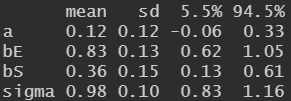
\includegraphics[scale=0.8]{descendant7_reg3.png}}]
	{How can I fix it???}
	
	\begin{figure}
		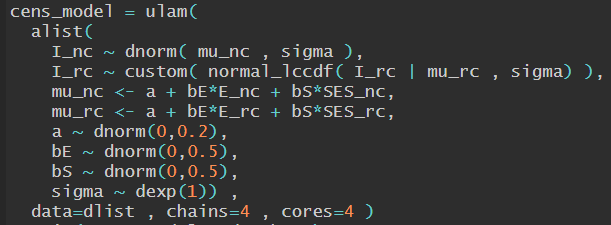
\includegraphics[scale=0.6]{descendant7_code2.png}
	\end{figure}
	%
	
	based on \textcolor{blue}{DAG} and \textcolor{blue}{statistical model},
	%
	\begin{itemize}
		%
		\item variables in two parts: \\
		$X_{nc}$ is the non-censored part, \\
		$X_{rc}$ is the right censored part 
		%
		\item Complementary Cumulative Normal $Nccd()$,
		%
		\item \textcolor{blue}{same parameters} for both parts
		%
	\end{itemize}
	%
\end{lhframe}
%
%
%%%%%%%%%%%%%%%%%%%%%%%%%%%%%%%%%%%%%%%%%%%%%%%%%%%%%%%%%%%
\subsection{Descendant: censoring, predictor only}
%%%%%%%%%%%%%%%%%%%%%%%%%%%%%%%%%%%%%%%%%%%%%%%%%%%%%%%%%%%
%
%
\begin{frame}[t, negative]
	\subsectionpage
\end{frame}
%
%	
\begin{frame}
	{Censoring, predictor only}
	%
	\begin{columns}
		%
		\begin{column}{0.5\textwidth}
			%
			research question, 
			%
			\begin{itemize}
				%
				\item \textcolor{blue}{Does $E$ has a (direct) effect on $I$?}
				%
			\end{itemize}
			
			variables,
			%
			\begin{itemize}
				%
				\item SES, socio economical status
				\item Ef, education (\textit{fully observed})
				\item Ec, education (\textit{left censored})
				\item I, income 
				%
			\end{itemize}
			%
			
			extras,
			%
			\begin{itemize}
				%
				\item $U_{I}$, between variability
				\item $U_{C}$, censoring mechanism
				%
			\end{itemize}
			%
		\end{column}
		%
		\begin{column}{0.5\textwidth}  
			%
			\begin{equ}
				%
				M = \left\{ \begin{aligned} 
					SES \leftarrow & \; f_{S}(U_{S}) \\
					Ef \leftarrow & \; f_{E}(SES,U_{E}) \\
					Ec \leftarrow & \; f_{E}(Ef, U_{C}) \\
					I \leftarrow & \; f_{I}(Ef, SES, U_{I}) \\
					U \sim & \; P(\pmb{U})
					%
				\end{aligned} \right
				%
				\caption*{(a) structural model}
				%
			\end{equ}
			%
			\begin{figure}
				%
				\begin{tikzpicture}
					% nodes
					\node[formula] at (-2.6,0.7) {$U_{C}$};
					\node[formula] at (-2,-0.3) {$Ec$};
					\node[formula] at (-1.7,0.7) {$U_{E}$};
					\node[formula] at (-1,-0.3) {$Ef$};
					\node[formula] at (1,1.5) {$U_{S}$};
					\node[formula] at (-0.3,1) {$SES$};
					\node[formula] at (2,0) {$U_{I}$};
					\node[formula] at (1,-0.3) {$I$};
					
					% paths
					\draw [{Circle [open]}-{latex}](-1.6,0.45)--(-1.05,0.05); % Ue->Ef
					\draw [-{latex}](-0.9,0)--(0.9,0); % Ef->I
					\draw [{Circle[open]}-{latex}{Circle}](-0.9,0)--(-2,0); % Ef->Ec
					\draw [{Circle [open]}-{latex}](-2.5,0.45)--(-2,0.05); % Uc->Ec
					\draw [{Circle [open]}-{latex}{Circle}](1.7,0)--(0.9,0); % Ui->I
					\draw [{Circle [color=red]}-{latex}](0.1,0.8)--(-0.9,0.1); % SES->Ef
					\draw [-{latex}](0.1,0.75)--(0.9,0.1); % SES->I
					\draw [{Circle [open]}-{latex}](0.9,1.3)--(0.1,0.8); % Us->S
					
					% extra
					\node at (0,-0.25) {$(?)$}; % symbol
				\end{tikzpicture}
				%
				\caption*{(b) causal diagram}
				%
			\end{figure}
			%
		\end{column}
		%
	\end{columns}
	%
\end{frame}
%
%
\begin{frame}
	{Simulation setting}
	%
	\begin{columns}
		%
		\begin{column}{0.5\textwidth}
			%
			\begin{figure}
				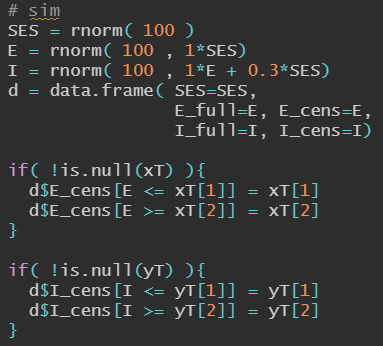
\includegraphics[scale=0.65]{descendant7_code.png}
				\caption*{(c) R code}
			\end{figure}
			%
			\textcolor{blue}{Implications},
			%
			\begin{itemize}
				\item \ndsep{Ef}{I} \\
				\item \ndsep{Ef}{I} \; | SES {\small (not possible)}
			\end{itemize}
			%
		\end{column}
		%
		\begin{column}{0.5\textwidth}  
			%
			\begin{equ}
				%
				M = \left\{ \begin{aligned} 
					SES \leftarrow & \; f_{S}(U_{S}) \\
					Ef \leftarrow & \; f_{E}(SES,U_{E}) \\
					Ec \leftarrow & \; f_{E}(Ef, U_{C}) \\
					I \leftarrow & \; f_{I}(Ef, SES, U_{I}) \\
					U \sim & \; P(\pmb{U})
					%
				\end{aligned} \right
				%
				\caption*{(a) structural model}
				%
			\end{equ}
			%
			\begin{figure}
				%
				\begin{tikzpicture}
					% nodes
					\node[formula] at (-2.6,0.7) {$U_{C}$};
					\node[formula] at (-2,-0.3) {$Ec$};
					\node[formula] at (-1.7,0.7) {$U_{E}$};
					\node[formula] at (-1,-0.3) {$Ef$};
					\node[formula] at (1,1.5) {$U_{S}$};
					\node[formula] at (-0.3,1) {$SES$};
					\node[formula] at (2,0) {$U_{I}$};
					\node[formula] at (1,-0.3) {$I$};
					
					% paths
					\draw [{Circle [open]}-{latex}](-1.6,0.45)--(-1.05,0.05); % Ue->Ef
					\draw [-{latex}](-0.9,0)--(0.9,0); % Ef->I
					\draw [{Circle[open]}-{latex}{Circle}](-0.9,0)--(-2,0); % Ef->Ec
					\draw [{Circle [open]}-{latex}](-2.5,0.45)--(-2,0.05); % Uc->Ec
					\draw [{Circle [open]}-{latex}{Circle}](1.7,0)--(0.9,0); % Ui->I
					\draw [{Circle [color=red]}-{latex}](0.1,0.8)--(-0.9,0.1); % SES->Ef
					\draw [-{latex}](0.1,0.75)--(0.9,0.1); % SES->I
					\draw [{Circle [open]}-{latex}](0.9,1.3)--(0.1,0.8); % Us->S
				\end{tikzpicture}
				%
				\caption*{(b) causal diagram}
				%
			\end{figure}
			%
		\end{column}
		%
	\end{columns}
	%
\end{frame}
%
%
\begin{frame}
	{So, what does the simulation means?}
	
	\begin{figure*}
		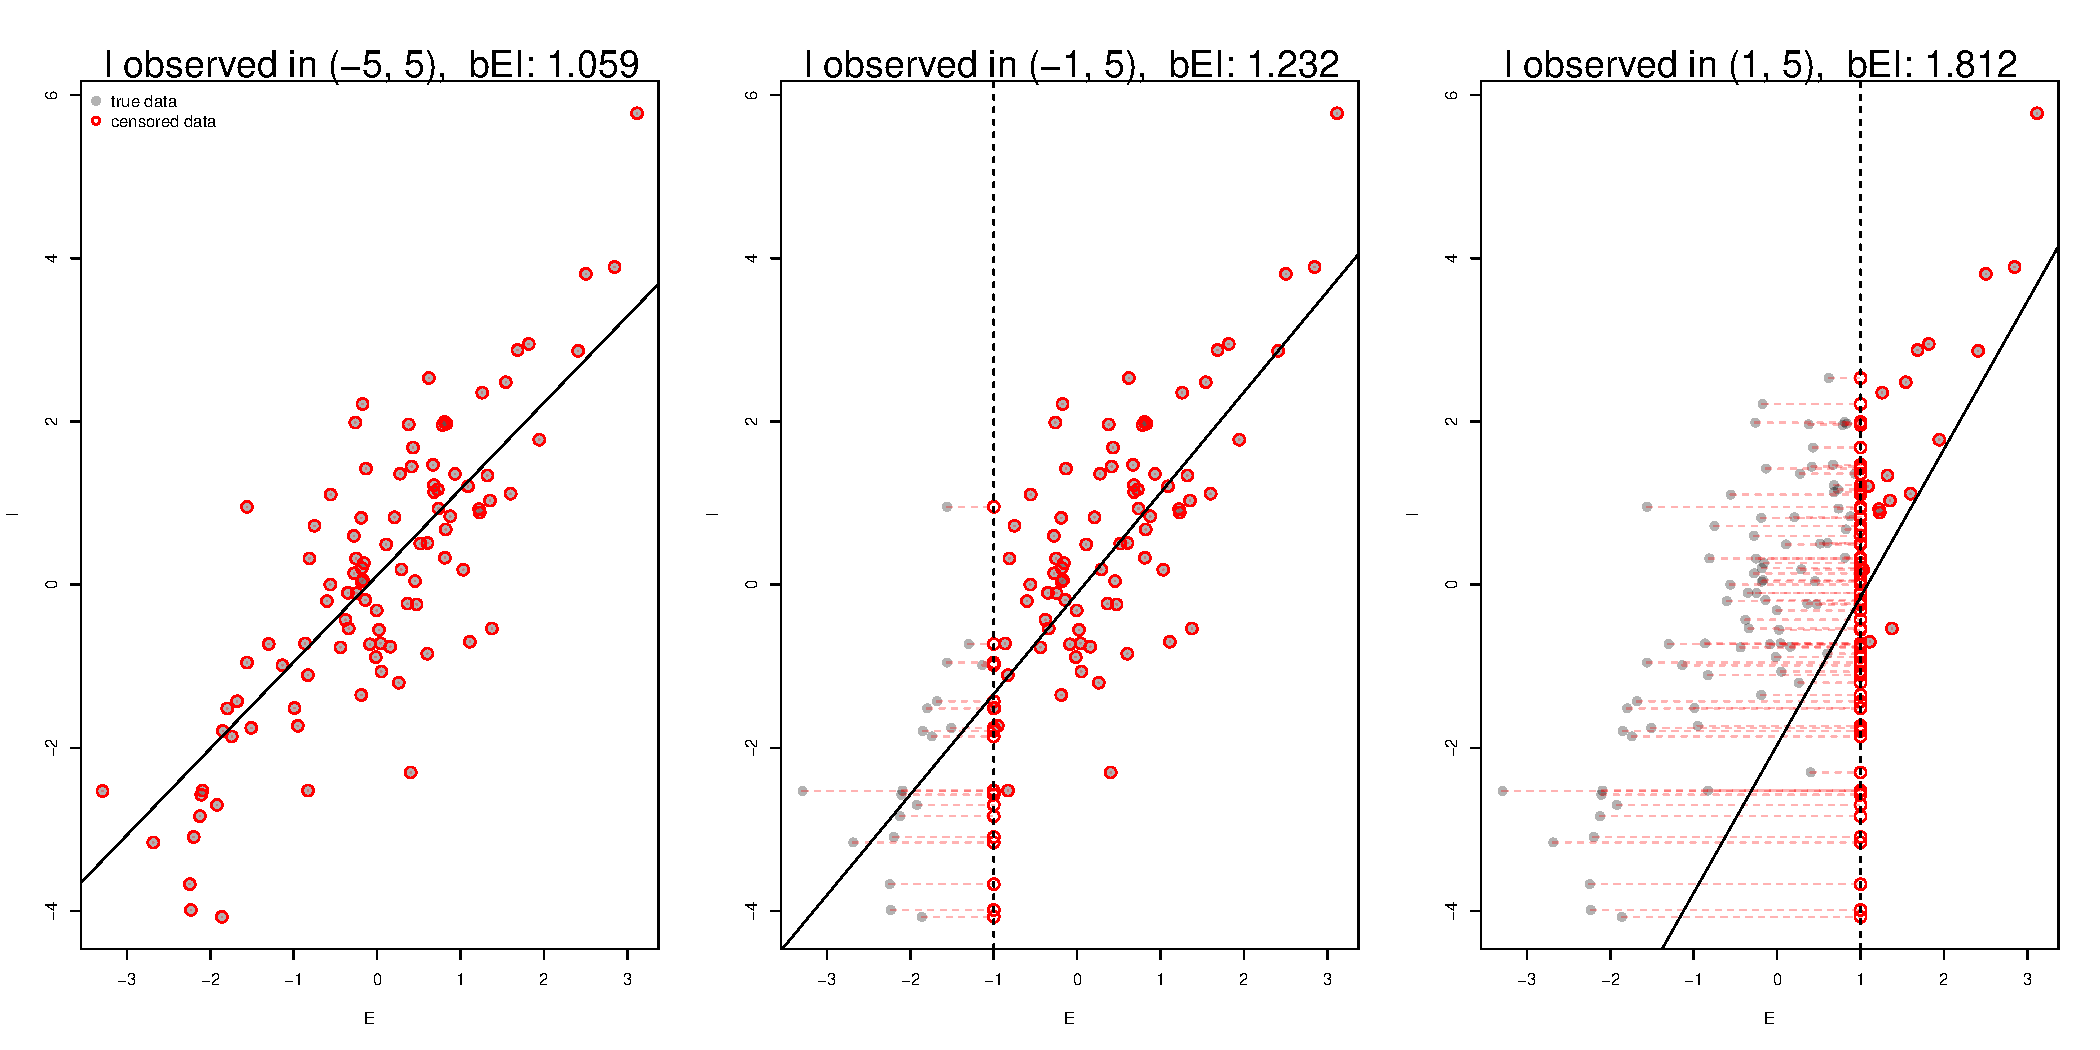
\includegraphics[width=\linewidth]{descendant8_cens1.pdf}
	\end{figure*}
	%
\end{frame}
%
%
\begin{frame}
	{So, what does the simulation means?}
	
	\begin{figure*}
		\includegraphics[width=\linewidth]{descendant8_cens2.pdf}
	\end{figure*}
	%
\end{frame}
%
%
\begin{lhframe}[rhgraphic={\includegraphics[scale=0.4]{descendant8_panel.pdf}}]
	{``Eyeballing" analysis}
	
	\begin{itemize}
		\item does \textcolor{blue}{correlation analysis} help now?
		\item and how about \textcolor{blue}{step-wise regression?} \\
		\item \textcolor{blue}{highly skewed distribution} of the predictor, so what?
	\end{itemize}
	
\end{lhframe}
%
%
\begin{lhframe}[rhgraphic={\includegraphics[scale=0.3]{descendant8_reg.png}}]
	{Regression, regression!!}
	
	based on \textcolor{blue}{statistical analysis},
	%
	\begin{itemize}
		%
		\item first model is impossible (\textcolor{blue}{unobservable})
		\item effect \textcolor{blue}{bias} in \textcolor{blue}{censored} data \\
		(E and SES)
		\item we have \textcolor{blue}{larger} standard errors \\
		{\small (why?? hint: ``synthetic'' larger variability in predictor)}
		%
	\end{itemize}
	%
\end{lhframe}
%
%
\begin{lhframe}[rhgraphic={\includegraphics[scale=0.45]{descendant8_samplesize.pdf}}]
	{So, what is going on?}
	
	imagine we can continue sampling,
	%
	\begin{itemize}
		%
		\item $10,000$ samples $n=100$
		%
	\end{itemize}
	
	notice,
	%
	\begin{itemize}
		%
		\item the smaller the \textcolor{blue}{censoring range}, the \textcolor{blue}{less confident} you are of your estimates,
		%
		\item smaller \textcolor{blue}{censoring range} the larger the \textcolor{blue}{bias} in effects, \\
		{\small (also for SES, not shown)}
		%
	\end{itemize}
	%
\end{lhframe}
%
%

\begin{comment}

\begin{frame}
	{How can I fix it???}
	%
	\begin{columns}
		%
		\begin{column}{0.5\textwidth}
			%
			\begin{equ}
				%
				\begin{aligned} 
					I_{nc} \sim & \; N( \mu_{nc} , \sigma_{I} ) \\
					\mu_{nc} = & \; \alpha + \beta_{E} E_{nc} + \beta_{S} SES_{nc} \\
					I_{rc} \sim & \; Nccd( \mu_{rc} , \sigma_{I} ) \\
					\mu_{rc} = & \; \alpha + \beta_{E} E_{rc} + \beta_{S} SES_{rc}
				\end{aligned}
				%
				\caption*{(c) probabilistic model}
				%
			\end{equ}
			%
			based on \textcolor{blue}{DAG} and \textcolor{blue}{statistical model},
			%
			\begin{itemize}
				%
				\item variables in two parts: \\
				$X_{nc}$ is the non-censored part, \\
				$X_{rc}$ is the right censored part 
				%
				\item Complementary Cumulative Normal $Nccd()$,
				%
				\item \textcolor{blue}{same parameters} for both parts
				%
			\end{itemize}
			%
		\end{column}
		%
		\begin{column}{0.5\textwidth}  
			%
			\begin{equ}
				%
				M = \left\{ \begin{aligned} 
					SES \leftarrow & \; f_{S}(U_{S}) \\
					Ef \leftarrow & \; f_{E}(SES,U_{E}) \\
					Ec \leftarrow & \; f_{E}(Ef, U_{C}) \\
					I \leftarrow & \; f_{I}(Ef, SES, U_{I}) \\
					U \sim & \; P(\pmb{U})
					%
				\end{aligned} \right
				%
				\caption*{(a) structural model}
				%
			\end{equ}
			%
			\begin{figure}
				%
				\begin{tikzpicture}
					% nodes
					\node[formula] at (-2.6,0.7) {$U_{C}$};
					\node[formula] at (-2,-0.3) {$Ec$};
					\node[formula] at (-1.7,0.7) {$U_{E}$};
					\node[formula] at (-1,-0.3) {$Ef$};
					\node[formula] at (1,1.5) {$U_{S}$};
					\node[formula] at (-0.3,1) {$SES$};
					\node[formula] at (2,0) {$U_{I}$};
					\node[formula] at (1,-0.3) {$I$};
					
					% paths
					\draw [{Circle [open]}-{latex}](-1.6,0.45)--(-1.05,0.05); % Ue->Ef
					\draw [-{latex}](-0.9,0)--(0.9,0); % Ef->I
					\draw [{Circle[open]}-{latex}{Circle}](-0.9,0)--(-2,0); % Ef->Ec
					\draw [{Circle [open]}-{latex}](-2.5,0.45)--(-2,0.05); % Uc->Ec
					\draw [{Circle [open]}-{latex}{Circle}](1.7,0)--(0.9,0); % Ui->I
					\draw [{Circle [color=red]}-{latex}](0.1,0.8)--(-0.9,0.1); % SES->Ef
					\draw [-{latex}](0.1,0.75)--(0.9,0.1); % SES->I
					\draw [{Circle [open]}-{latex}](0.9,1.3)--(0.1,0.8); % Us->S
					
					% extra
					\node at (0,-0.25) {$(?)$}; % symbol
				\end{tikzpicture}
				%
				\caption*{(b) causal diagram}
				%
			\end{figure}
			%
		\end{column}
		%
	\end{columns}
	%
\end{frame}
%
%
\begin{lhframe}[rhgraphic={\includegraphics[scale=0.8]{descendant7_reg3.png}}]
	{How can I fix it???}
	
	\begin{figure}
		\includegraphics[scale=0.6]{descendant7_code2.png}
	\end{figure}
	%
	
	based on \textcolor{blue}{DAG} and \textcolor{blue}{statistical model},
	%
	\begin{itemize}
		%
		\item variables in two parts: \\
		$X_{nc}$ is the non-censored part, \\
		$X_{rc}$ is the right censored part 
		%
		\item Complementary Cumulative Normal $Nccd()$,
		%
		\item \textcolor{blue}{same parameters} for both parts
		%
	\end{itemize}
	%
\end{lhframe}

\end{comment}
%
%
%%%%%%%%%%%%%%%%%%%%%%%%%%%%%%%%%%%%%%%%%%%%%%%%%%%%%%%%%%%
\subsection{Descendant: censoring, both}
%%%%%%%%%%%%%%%%%%%%%%%%%%%%%%%%%%%%%%%%%%%%%%%%%%%%%%%%%%%
%
%
\begin{frame}[t, negative]
	\subsectionpage
\end{frame}
%
%	
\begin{frame}
	{Censoring, both}
	%
	\begin{columns}
		%
		\begin{column}{0.5\textwidth}
			%
			research question, 
			%
			\begin{itemize}
				%
				\item \textcolor{blue}{Does $E$ has a (direct) effect on $I$?}
				%
			\end{itemize}
			
			variables,
			%
			\begin{itemize}
				%
				\item SES, socio economical status
				\item Ef, education (\textit{fully observed})
				\item Ec, education (\textit{left censored})
				\item If, income (\textit{fully observed})
				\item Ic, income (\textit{censored})
				%
			\end{itemize}
			%
			
			extras,
			%
			\begin{itemize}
				%
				\item $U_{I}$, between variability
				\item $U_{E}$, between variability
				\item $U_{C1}$, censoring mechanism (E)
				\item $U_{C2}$, censoring mechanism (I)
				%
			\end{itemize}
			%
		\end{column}
		%
		\begin{column}{0.5\textwidth}  
			%
			\begin{equ}
				%
				M = \left\{ \begin{aligned} 
					SES \leftarrow & \; f_{S}(U_{S}) \\
					Ef \leftarrow & \; f_{E}(SES,U_{E}) \\
					Ec \leftarrow & \; f_{E}(Ef, U_{C1}) \\
					If \leftarrow & \; f_{I}(SES, Ef, U_{I}) \\
					Ic \leftarrow & \; f_{I}(If, U_{C2}) \\
					U \sim & \; P(\pmb{U})
					%
				\end{aligned} \right
				%
				\caption*{(a) structural model}
				%
			\end{equ}
			%
			\begin{figure}
				%
				\begin{tikzpicture}
					% nodes
					\node[formula] at (-2.6,0.7) {$U_{C1}$};
					\node[formula] at (-2,-0.3) {$Ec$};
					\node[formula] at (-1.7,0.7) {$U_{E}$};
					\node[formula] at (-1,-0.3) {$Ef$};
					\node[formula] at (1,1.5) {$U_{S}$};
					\node[formula] at (-0.2,1) {$SES$};
					\node[formula] at (1.8,0.7) {$U_{I}$};
					\node[formula] at (1,-0.3) {$If$};
					\node[formula] at (2.7,0.7) {$U_{C2}$};
					\node[formula] at (1.95,-0.3) {$Ic$};
					
					% paths
					\draw [{Circle [open]}-{latex}](-1.6,0.45)--(-1.05,0.05); % UE->Ef
					\draw [-{latex}](-0.9,0)--(0.9,0); % Ef->If
					\draw [{Circle [open]}-{latex}{Circle}](0.9,0)--(2,0); % If->Ec
					\draw [{Circle [open]}-{latex}](1.7,0.5)--(1.05,0.05); % Ui->If
					\draw [{Circle [open]}-{latex}](2.6,0.5)--(2,0.05); % Uc2->Ic
					\draw [{Circle[open]}-{latex}{Circle}](-0.9,0)--(-2,0); % Ef->Ec
					\draw [{Circle [open]}-{latex}](-2.5,0.45)--(-2,0.05); % Uc1->Ec
					\draw [{Circle [color=red]}-{latex}](0.1,0.8)--(-0.9,0.1); % SES->Ef
					\draw [-{latex}](0.1,0.75)--(0.9,0.1); % SES->If
					\draw [{Circle [open]}-{latex}](0.9,1.3)--(0.1,0.8); % Us->SES
					
					% extra
					\node at (0,-0.25) {$(?)$}; % symbol
				\end{tikzpicture}
				%
				\caption*{(b) causal diagram}
				%
			\end{figure}
			%
		\end{column}
		%
	\end{columns}
	%
\end{frame}
%
%
\begin{frame}
	{Simulation setting}
	%
	\begin{columns}
		%
		\begin{column}{0.5\textwidth}
			%
			\begin{figure}
				\includegraphics[scale=0.65]{descendant7_code.png}
				\caption*{(c) R code}
			\end{figure}
			%
			\textcolor{blue}{Implications},
			%
			\begin{itemize}
				\item \ndsep{Ef}{I} \\
				\item \ndsep{Ef}{I} \; | SES {\small (not possible)}
			\end{itemize}
			%
		\end{column}
		%
		\begin{column}{0.5\textwidth}  
			%
			\begin{equ}
				%
				M = \left\{ \begin{aligned} 
					SES \leftarrow & \; f_{S}(U_{S}) \\
					Ef \leftarrow & \; f_{E}(SES,U_{E}) \\
					Ec \leftarrow & \; f_{E}(Ef, U_{C1}) \\
					If \leftarrow & \; f_{I}(SES, Ef, U_{I}) \\
					Ic \leftarrow & \; f_{I}(If, U_{C2}) \\
					U \sim & \; P(\pmb{U})
					%
				\end{aligned} \right
				%
				\caption*{(a) structural model}
				%
			\end{equ}
			%
			\begin{figure}
				%
				\begin{tikzpicture}
					% nodes
					\node[formula] at (-2.6,0.7) {$U_{C1}$};
					\node[formula] at (-2,-0.3) {$Ec$};
					\node[formula] at (-1.7,0.7) {$U_{E}$};
					\node[formula] at (-1,-0.3) {$Ef$};
					\node[formula] at (1,1.5) {$U_{S}$};
					\node[formula] at (-0.2,1) {$SES$};
					\node[formula] at (1.8,0.7) {$U_{I}$};
					\node[formula] at (1,-0.3) {$If$};
					\node[formula] at (2.7,0.7) {$U_{C2}$};
					\node[formula] at (1.95,-0.3) {$Ic$};
					
					% paths
					\draw [{Circle [open]}-{latex}](-1.6,0.45)--(-1.05,0.05); % UE->Ef
					\draw [-{latex}](-0.9,0)--(0.9,0); % Ef->If
					\draw [{Circle [open]}-{latex}{Circle}](0.9,0)--(2,0); % If->Ec
					\draw [{Circle [open]}-{latex}](1.7,0.5)--(1.05,0.05); % Ui->If
					\draw [{Circle [open]}-{latex}](2.6,0.5)--(2,0.05); % Uc2->Ic
					\draw [{Circle[open]}-{latex}{Circle}](-0.9,0)--(-2,0); % Ef->Ec
					\draw [{Circle [open]}-{latex}](-2.5,0.45)--(-2,0.05); % Uc1->Ec
					\draw [{Circle [color=red]}-{latex}](0.1,0.8)--(-0.9,0.1); % SES->Ef
					\draw [-{latex}](0.1,0.75)--(0.9,0.1); % SES->If
					\draw [{Circle [open]}-{latex}](0.9,1.3)--(0.1,0.8); % Us->SES
				\end{tikzpicture}
				%
				\caption*{(b) causal diagram}
				%
			\end{figure}
			%
		\end{column}
		%
	\end{columns}
	%
\end{frame}
%
%
\begin{frame}
	{So, what does the simulation means?}
	
	\begin{figure*}
		\includegraphics[width=\linewidth]{descendant9_cens1.pdf}
	\end{figure*}
	%
\end{frame}
%
%
\begin{frame}
	{So, what does the simulation means?}
	
	\begin{figure*}
		\includegraphics[width=\linewidth]{descendant9_cens2.pdf}
	\end{figure*}
	%
\end{frame}
%
%
\begin{lhframe}[rhgraphic={\includegraphics[scale=0.4]{descendant9_panel.pdf}}]
	{``Eyeballing" analysis}
	
	\begin{itemize}
		\item does \textcolor{blue}{correlation analysis} help now?
		\item and how about \textcolor{blue}{step-wise regression?} \\
		\item \textcolor{blue}{highly skewed distribution} of the predictor, so what?
		\item notice the \textcolor{blue}{high dependence} between E and I \\
		{\small \alert{(this is the thing of nightmares!!)}}
	\end{itemize}
	
\end{lhframe}
%
%
\begin{lhframe}[rhgraphic={\includegraphics[scale=0.3]{descendant9_reg.png}}]
	{Regression, regression!!}
	
	based on \textcolor{blue}{statistical analysis},
	%
	\begin{itemize}
		%
		\item first model is impossible (\textcolor{blue}{unobservable})
		\item \alert{no comment on the rest} \\
		{\small (why?? hint: I'm having a breakdown)}
		%
	\end{itemize}
	%
\end{lhframe}
%
%
\begin{lhframe}[rhgraphic={\includegraphics[scale=0.45]{descendant9_samplesize.pdf}}]
	{So, what is going on?}
	
	imagine we can continue sampling,
	%
	\begin{itemize}
		%
		\item $10,000$ samples $n=100$
		%
	\end{itemize}
	
	notice,
	%
	\begin{itemize}
		%
		\item \textcolor{blue}{no clear direction} for the biasing of effects, when the \textcolor{blue}{censoring range} changes
		%
	\end{itemize}
	%
\end{lhframe}
%
%

\begin{comment}
	
	\begin{frame}
		{How can I fix it???}
		%
		\begin{columns}
			%
			\begin{column}{0.5\textwidth}
				%
				\begin{equ}
					%
					\begin{aligned} 
						I_{nc} \sim & \; N( \mu_{nc} , \sigma_{I} ) \\
						\mu_{nc} = & \; \alpha + \beta_{E} E_{nc} + \beta_{S} SES_{nc} \\
						I_{rc} \sim & \; Nccd( \mu_{rc} , \sigma_{I} ) \\
						\mu_{rc} = & \; \alpha + \beta_{E} E_{rc} + \beta_{S} SES_{rc}
					\end{aligned}
					%
					\caption*{(c) probabilistic model}
					%
				\end{equ}
				%
				based on \textcolor{blue}{DAG} and \textcolor{blue}{statistical model},
				%
				\begin{itemize}
					%
					\item variables in two parts: \\
					$X_{nc}$ is the non-censored part, \\
					$X_{rc}$ is the right censored part 
					%
					\item Complementary Cumulative Normal $Nccd()$,
					%
					\item \textcolor{blue}{same parameters} for both parts
					%
				\end{itemize}
				%
			\end{column}
			%
			\begin{column}{0.5\textwidth}  
				%
				\begin{equ}
					%
					M = \left\{ \begin{aligned} 
						SES \leftarrow & \; f_{S}(U_{S}) \\
						Ef \leftarrow & \; f_{E}(SES,U_{E}) \\
						Ec \leftarrow & \; f_{E}(Ef, U_{C}) \\
						I \leftarrow & \; f_{I}(Ef, SES, U_{I}) \\
						U \sim & \; P(\pmb{U})
						%
					\end{aligned} \right
					%
					\caption*{(a) structural model}
					%
				\end{equ}
				%
				\begin{figure}
					%
					\begin{tikzpicture}
						% nodes
						\node[formula] at (-2.6,0.7) {$U_{C}$};
						\node[formula] at (-2,-0.3) {$Ec$};
						\node[formula] at (-1.7,0.7) {$U_{E}$};
						\node[formula] at (-1,-0.3) {$Ef$};
						\node[formula] at (1,1.5) {$U_{S}$};
						\node[formula] at (-0.3,1) {$SES$};
						\node[formula] at (2,0) {$U_{I}$};
						\node[formula] at (1,-0.3) {$I$};
						
						% paths
						\draw [{Circle [open]}-{latex}](-1.6,0.45)--(-1.05,0.05); % Ue->Ef
						\draw [-{latex}](-0.9,0)--(0.9,0); % Ef->I
						\draw [{Circle[open]}-{latex}{Circle}](-0.9,0)--(-2,0); % Ef->Ec
						\draw [{Circle [open]}-{latex}](-2.5,0.45)--(-2,0.05); % Uc->Ec
						\draw [{Circle [open]}-{latex}{Circle}](1.7,0)--(0.9,0); % Ui->I
						\draw [{Circle [color=red]}-{latex}](0.1,0.8)--(-0.9,0.1); % SES->Ef
						\draw [-{latex}](0.1,0.75)--(0.9,0.1); % SES->I
						\draw [{Circle [open]}-{latex}](0.9,1.3)--(0.1,0.8); % Us->S
						
						% extra
						\node at (0,-0.25) {$(?)$}; % symbol
					\end{tikzpicture}
					%
					\caption*{(b) causal diagram}
					%
				\end{figure}
				%
			\end{column}
			%
		\end{columns}
		%
	\end{frame}
	%
	%
	\begin{lhframe}[rhgraphic={\includegraphics[scale=0.8]{descendant7_reg3.png}}]
		{How can I fix it???}
		
		\begin{figure}
			\includegraphics[scale=0.6]{descendant7_code2.png}
		\end{figure}
		%
		
		based on \textcolor{blue}{DAG} and \textcolor{blue}{statistical model},
		%
		\begin{itemize}
			%
			\item variables in two parts: \\
			$X_{nc}$ is the non-censored part, \\
			$X_{rc}$ is the right censored part 
			%
			\item Complementary Cumulative Normal $Nccd()$,
			%
			\item \textcolor{blue}{same parameters} for both parts
			%
		\end{itemize}
		%
	\end{lhframe}
	
\end{comment}
%
%

\begin{comment}

%%%%%%%%%%%%%%%%%%%%%%%%%%%%%%%%%%%%%%%%%%%%%%%%%%%%%%%%%%%
\subsection{Descendant: truncation, outcome only}
%%%%%%%%%%%%%%%%%%%%%%%%%%%%%%%%%%%%%%%%%%%%%%%%%%%%%%%%%%%
%
%
\begin{frame}[t, negative]
	\subsectionpage
\end{frame}
%
%	
\begin{frame}
	{Truncation, outcome only\footnote{\citet{Ostling_2022}, \citet{Vincent_2022} }}
	%
	\begin{columns}
		%
		\begin{column}{0.5\textwidth}
			%
			also, 
			%
			\begin{itemize}
				%
				\item special case of \textcolor{blue}{MAR missing data?}
				%
			\end{itemize}
		
			research question, 
			%
			\begin{itemize}
				%
				\item \textcolor{blue}{Does $E$ has a (direct) effect on $I$?}
				%
			\end{itemize}
			
			variables,
			%
			\begin{itemize}
				%
				\item SES, socio economical status
				\item E, education
				\item If, income (\textit{fully observed})
				\item It, income (\textit{truncated})
				%
			\end{itemize}
			%
			
			extras,
			%
			\begin{itemize}
				%
				\item $U_{I}$, between variability
				\item $U_{T}$, truncation mechanism
				%
			\end{itemize}
			%
		\end{column}
		%
		\begin{column}{0.5\textwidth}  
			%
			\begin{equ}
				%
				M = \left\{ \begin{aligned} 
					SES \leftarrow & \; f_{S}(U_{S}) \\
					E \leftarrow & \; f_{E}(SES,U_{E}) \\
					If \leftarrow & \; f_{I}(E, SES, U_{I}) \\
					It \leftarrow & \; f_{I}(If, U_{T}) \\
					U \sim & \; P(\pmb{U})
					%
				\end{aligned} \right
				%
				\caption*{(a) structural model}
				%
			\end{equ}
			%
			\begin{figure}
				%
				\begin{tikzpicture}
					% nodes
					\node[formula] at (-2,0) {$U_{E}$};
					\node[formula] at (-1,-0.3) {$E$};
					\node[formula] at (1,1.5) {$U_{S}$};
					\node[formula] at (-0.3,1) {$SES$};
					\node[formula] at (1.8,0.7) {$U_{I}$};
					\node[formula] at (1,-0.3) {$If$};
					\node[formula] at (2.7,0.7) {$U_{T}$};
					\node[formula] at (1.95,-0.3) {$It$};
					
					% paths
					\draw [{Circle [open]}-{latex}{Circle}](-1.7,0)--(-0.9,0); % Ue->E
					\draw [-{latex}](-0.9,0)--(0.9,0); % E->If
					\draw [{Circle [open]}-{latex}{Circle}](0.9,0)--(2,0); % If->It
					\draw [{Circle [open]}-{latex}](1.7,0.5)--(1.05,0.05); % Ui->If
					\draw [{Circle [open]}-{latex}](2.6,0.5)--(2,0.05); % Ut->It
					\draw [{Circle [color=red]}-{latex}](0.1,0.8)--(-0.9,0.1); % SES->E
					\draw [-{latex}](0.1,0.75)--(0.9,0.1); % SES->If
					\draw [{Circle [open]}-{latex}](0.9,1.3)--(0.1,0.8); % US->SES
					
					% extra
					\node at (0,-0.25) {$(?)$}; % symbol
				\end{tikzpicture}
				%
				\caption*{(b) causal diagram}
				%
			\end{figure}
			%
		\end{column}
		%
	\end{columns}
	%
\end{frame}
%
%
\begin{frame}
	{Simulation setting}
	%
	\begin{columns}
		%
		\begin{column}{0.5\textwidth}
			%
			\begin{figure}
				\includegraphics[scale=0.6]{descendant7_code.png}
				\caption*{(c) R code}
			\end{figure}
			%
			\textcolor{blue}{Implications},
			%
			\begin{itemize}
				\item \ndsep{E}{If} \\
				\item \ndsep{E}{If} \; | SES {\small (not possible)}
			\end{itemize}
			%
		\end{column}
		%
		\begin{column}{0.5\textwidth}  
			%
			\begin{equ}
				%
				M = \left\{ \begin{aligned} 
					SES \leftarrow & \; f_{S}(U_{S}) \\
					E \leftarrow & \; f_{E}(SES,U_{E}) \\
					If \leftarrow & \; f_{I}(E, SES, U_{I}) \\
					It \leftarrow & \; f_{I}(If, U_{T}) \\
					U \sim & \; P(\pmb{U})
					%
				\end{aligned} \right
				%
				\caption*{(a) structural model}
				%
			\end{equ}
			%
			\begin{figure}
				%
				\begin{tikzpicture}
					% nodes
					\node[formula] at (-2,0) {$U_{E}$};
					\node[formula] at (-1,-0.3) {$E$};
					\node[formula] at (1,1.5) {$U_{S}$};
					\node[formula] at (-0.3,1) {$SES$};
					\node[formula] at (1.8,0.7) {$U_{I}$};
					\node[formula] at (1,-0.3) {$If$};
					\node[formula] at (2.7,0.7) {$U_{T}$};
					\node[formula] at (1.95,-0.3) {$It$};
					
					% paths
					\draw [{Circle [open]}-{latex}{Circle}](-1.7,0)--(-0.9,0); % Ue->E
					\draw [-{latex}](-0.9,0)--(0.9,0); % E->If
					\draw [{Circle [open]}-{latex}{Circle}](0.9,0)--(2,0); % If->It
					\draw [{Circle [open]}-{latex}](1.7,0.5)--(1.05,0.05); % Ui->If
					\draw [{Circle [open]}-{latex}](2.6,0.5)--(2,0.05); % Ut->It
					\draw [{Circle [color=red]}-{latex}](0.1,0.8)--(-0.9,0.1); % SES->E
					\draw [-{latex}](0.1,0.75)--(0.9,0.1); % SES->If
					\draw [{Circle [open]}-{latex}](0.9,1.3)--(0.1,0.8); % US->SES
				\end{tikzpicture}
				%
				\caption*{(b) causal diagram}
				%
			\end{figure}
			%
		\end{column}
		%
	\end{columns}
	%
\end{frame}
%
%
\begin{frame}
	{So, what does the simulation means?}
	
	\begin{figure*}
		\includegraphics[width=\linewidth]{descendant7_trunc.pdf}
	\end{figure*}
	%
\end{frame}
%
%
\begin{lhframe}[rhgraphic={\includegraphics[scale=0.4]{descendant7_panel.pdf}}]
	{``Eyeballing" analysis}
	
	does \textcolor{blue}{correlation analysis} help now? \\
	and how about \textcolor{blue}{step-wise regression?}
\end{lhframe}
%
%
\begin{lhframe}[rhgraphic={\includegraphics[scale=0.3]{descendant7_reg.png}}]
	{Regression, regression!!}
	
	based on \textcolor{blue}{statistical analysis},
	%
	\begin{itemize}
		%
		\item first model is impossible (\textcolor{blue}{unobservable})
		\item \textcolor{blue}{huge} effect bias in \textcolor{blue}{truncated} data (E  and SES)
		\item we have \textcolor{blue}{larger} standard error \\
		{\small (we lose some observations)}
		%
	\end{itemize}
	%
\end{lhframe}
%
%
\begin{lhframe}[rhgraphic={\includegraphics[scale=0.45]{descendant7_samplesize.pdf}}]
	{So, what is going on?}
	
	imagine we can continue sampling,
	%
	\begin{itemize}
		%
		\item $10,000$ samples $n=100$
		%
	\end{itemize}
	
	notice,
	%
	\begin{itemize}
		%
		\item the larger the \textcolor{blue}{measurement error}, the \textcolor{blue}{more confident} you are of your estimates,
		%
		\item larger \textcolor{blue}{measurement error} (in predictor) \textcolor{blue}{hugely bias} the effects, \\
		{\small (also for A, not shown)}
		%
	\end{itemize}
	%
\end{lhframe}
%
%
\begin{frame}
	{How can I fix it???}
	%
	\begin{columns}
		%
		\begin{column}{0.5\textwidth}
			%
			\begin{equ}
				%
				\begin{aligned} 
					D \sim & \; N( \mu, \sigma_{D}) \\
					\mu = & \; \alpha + \beta_{AD} A + \beta_{MD} M_{true} \\
					M_{obs} \sim & \; N( M_{true}, \sigma_{O}) \\
					M_{true} \sim & \; N( 0, \sigma_{M})
				\end{aligned}
				%
				\caption*{(c) probabilistic model}
				%
			\end{equ}
			%
			based on \textcolor{blue}{DAG} and \textcolor{blue}{statistical model}, \\
			use the knowledge of the system
			%
			\begin{itemize}
				%
				\item measurement error part: $M_{obs} \sim N( M_{true}, \sigma_{O})$, 
				%
				\item latent structure: $M_{true} \sim N( 0, \sigma_{M} )$,
				%
				\item latent regression: $\mu = f(A, M_{true})$
				%
			\end{itemize}
			%
		\end{column}
		%
		\begin{column}{0.5\textwidth}  
			%
			\begin{equ}
				%
				M = \left\{ \begin{aligned} 
					A \leftarrow & \; f_{A}(U_{A}) \\
					Mt \leftarrow & \; f_{M}(A,U_{M}) \\
					Mo \leftarrow & \; f_{M}(Mt, U_{O}) \\
					D \leftarrow & \; f_{D}(A, Mt, U_{D}) \\
					U \sim & \; P(\pmb{U})
					%
				\end{aligned} \right
				%
				\caption*{(a) structural model}
				%
			\end{equ}
			%
			\begin{figure}
				%
				\begin{tikzpicture}
					% nodes
					\node[formula] at (-2.6,0.7) {$U_{O}$};
					\node[formula] at (-2,-0.3) {$Mo$};
					\node[formula] at (-1.7,0.7) {$U_{M}$};
					\node[formula] at (-1,-0.3) {$Mt$};
					\node[formula] at (1,1.5) {$U_{A}$};
					\node[formula] at (0,1) {$A$};
					\node[formula] at (2,0) {$U_{D}$};
					\node[formula] at (1,-0.3) {$D$};
					
					% paths
					\draw [{Circle [open]}-{latex}](-1.6,0.45)--(-1.05,0.05); % Um->Mt
					\draw [-{latex}](-0.9,0)--(0.9,0); % Mt->D
					\draw [{Circle[open]}-{latex}{Circle}](-0.9,0)--(-2,0); % Mt->Mo
					\draw [{Circle [open]}-{latex}](-2.5,0.45)--(-2,0.05); % Uo->Mo
					\draw [{Circle [open]}-{latex}{Circle}](1.7,0)--(0.9,0); % Ud->D
					\draw [{Circle [color=red]}-{latex}](0.1,0.8)--(-0.9,0.1); % A->M
					\draw [-{latex}](0.1,0.75)--(0.9,0.1); % A->D
					\draw [{Circle [open]}-{latex}](0.9,1.3)--(0.1,0.8); % Ua->A
					
					% extra
					\node at (0,-0.25) {$(?)$}; % symbol
				\end{tikzpicture}
				%
				\caption*{(b) causal diagram}
				%
			\end{figure}
			%
		\end{column}
		%
	\end{columns}
	%
\end{frame}
%
%
\begin{lhframe}[rhgraphic={\includegraphics[scale=0.8]{descendant7_reg3.png}}]
	{How can I fix it???}
	
	\begin{figure}
		\includegraphics[scale=0.7]{descendant7_code2.png}
	\end{figure}
	%
	
	Using \textcolor{blue}{DAG} and \textcolor{blue}{Bayesian} analysis: \\
	{\small \textcolor{blue}{(frequentist analysis falls short here)}}
	%
	\begin{itemize}
		%
		\item measurement error part: $M_{obs} \sim N( M_{true}, \sigma_{O})$, 
		%
		\item latent structure: $M_{true} \sim N( 0, \sigma_{M} )$,
		%
		\item latent regression: $\mu = f(A, M_{true})$
		%
	\end{itemize}
	%
\end{lhframe}
%
%

\end{comment}